\documentclass[a4paper,12pt,openany,oneside,utf-8]{ctexbook}
%\documentclass[a4paper,12pt,openany,oneside,utf-8]{cctbook}
%\usepackage{hyperref}
%\hypersetup{CJKbookmarks=true}
\usepackage{amssymb,amsmath}
\usepackage{subcaption}
\usepackage[amsmath,thmmarks]{ntheorem}
\usepackage{fancyhdr}
\usepackage{graphicx}
\usepackage{titletoc}%自己添加,
\usepackage{epsfig,picins,picinpar}
\usepackage{setspace}
%\usepackage[top=2.54cm,bottom=2.54cm,left=2.54cm,right=2.54cm]{geometry}
\usepackage{geometry}
\geometry{left=3.3cm,right=2.8cm,top=2.5cm,bottom=2.2cm,}
\usepackage{amsmath}
\usepackage{mathtools} % offer \coloneqq to show := [see https://tex.stackexchange.com/questions/194344/symbol-for-definition]
%%%%%%%%%%%%%%%%%%%%%%%%new
\usepackage[super,square,comma,sort&compress]{natbib}
\usepackage{multirow}
\usepackage{dsfont}
\usepackage{booktabs}
\usepackage{epstopdf}
\usepackage{ccmap}
\bibliographystyle{gbt7714-2005}%{elsarticle-num}%{elsarticle-num}%{plain}%{elsarticle-num-names}%




%%%%%%%%%%%%%%%%%%%%%%自己的导言区
%\usepackage{natbib}     % adding a package for \citet{}, \citep{}, \citet*{}, \citep*{}
\usepackage{amssymb} %% The amssymb package provides various useful mathematical symbols
\usepackage{amsmath}
\DeclareMathOperator*{\argmax}{arg\,max}
\usepackage{bm}         % adding a package for \bm{\widehat{\beta}}
\usepackage{makecell}   % makecell, see: https://blog.csdn.net/cy_tec/article/details/51436434
\usepackage{multirow}   % Latex Table, see: https://blog.csdn.net/canhui_wang/article/details/72920963
\usepackage{booktabs}   % for \cmidrule, see: https://zhidao.baidu.com/question/306414034088577164.html
\usepackage{graphicx}   % adding a package for loading figures
\usepackage{threeparttable}   % adding a package for tablenotes
\usepackage{algorithm}
\usepackage{algorithmicx}
\usepackage{algpseudocode}
\usepackage{titlesec}    % for \titleformat
\usepackage{indentfirst}   % 关于首个段落缩进的问题,可以在导言区加入宏包\usepackage{indentfirst}会自动缩进, see: https://zhidao.baidu.com/question/207438548.html
\usepackage{caption}   % for \captionsetup, see: https://blog.csdn.net/kebu12345678/article/details/76957377?locationNum=9&fps=1
\usepackage{makecell}  % for \Xcline  \Xhline, see: http://blog.sina.com.cn/s/blog_5e16f1770100mvtd.html
\floatname{algorithm}{Algorithm}  % Ref: https://blog.csdn.net/lwb102063/article/details/53046265
\renewcommand{\algorithmicrequire}{\textbf{Input:}}
\renewcommand{\algorithmicensure}{\textbf{Output:}}
\usepackage{paralist} % for \begin{enumerate}, see: http://bbs.ctex.org/forum.php?mod=viewthread&tid=62084
%%%%%%%%%%%%%%%%%%%%%%自己的导言区



%%%%%%%%%%%%%%%%%%%%%%%%
%\renewcommand\sectionname{\arabic{section}}
%\renewcommand\sectionformat{\centering}
%\renewcommand\subsectionname{\arabic{section}.\arabic{subsection}}
%\renewcommand\subsectionformat{}
%\renewcommand\subsubsectionname{\arabic{section}.\arabic{subsection}.\arabic{subsubsection}}
%\renewcommand\subsubsectionformat{}

\allowdisplaybreaks[4]
\renewcommand{\baselinestretch}{1.5}
%\renewcommand{\chaptername}{{Chapter\thechapter}}
\renewcommand{\chaptername}{第{\thechapter}章}
\renewcommand\bibname{参考文献}
\renewcommand\contentsname{目录}
%\renewcommand{\sectionname}{{\thechapter}.\arabic{section}}

\renewcommand {\thetable} {\thechapter{}-\arabic{table}} 
\renewcommand {\thefigure} {\thechapter{}-\arabic{figure}}

% 字体大小设置
\newcommand{\chuhao}{\fontsize{48pt}{\baselineskip}\selectfont}
\newcommand{\xiaochuhao}{\fontsize{36pt}{\baselineskip}\selectfont}
\newcommand{\yihao}{\fontsize{28pt}{\baselineskip}\selectfont}
\newcommand{\xiaoyihao}{\fontsize{25pt}{\baselineskip}\selectfont}
\newcommand{\erhao}{\fontsize{21pt}{\baselineskip}\selectfont}
\newcommand{\xiaoerhao}{\fontsize{17pt}{\baselineskip}\selectfont}
\newcommand{\sanhao}{\fontsize{15.75pt}{\baselineskip}\selectfont}
\newcommand{\xiaosanhao}{\fontsize{15pt}{\baselineskip}\selectfont}
\newcommand{\sihao}{\fontsize{13pt}{\baselineskip}\selectfont}
\newcommand{\xiaosihao}{\fontsize{12pt}{\baselineskip}\selectfont}
\newcommand{\wuhao}{\fontsize{10.5pt}{\baselineskip}\selectfont}
\newcommand{\xiaowuhao}{\fontsize{9pt}{\baselineskip}\selectfont}
\newcommand{\liuhao}{\fontsize{7.875pt}{\baselineskip}\selectfont}
\newcommand{\qihao}{\fontsize{5.25pt}{\baselineskip}\selectfont}%\newcommand\kaishu{\CJKfamily{kai}}
%这样在文档中就可以随心所欲地改变字体了, 比如上图中开始部分就是用
% {\yihao 1770年}{\sanhao 法国人狄道} 来实现的

\CTEXsetup[name={第,章}, number=\arabic{chapter}]{chapter} %将目录和正文的"第一章  XXXX"的输出格式改为"第1章 XXXX" see: https://blog.csdn.net/jk123vip/article/details/57163786 and http://tieba.baidu.com/p/3631630597
\titleformat{\chapter}{\centering\sanhao\bfseries}{第\,\thechapter\,章}{1em}{}
\titlespacing*{\chapter} {0pt}{-10.5pt}{12pt}

\titleformat{\section}{\centering\xiaosanhao\bfseries}{\thesection}{1em}{}
\titlespacing*{\section} {0pt}{12pt}{12pt}

\titleformat{\subsection}{\sihao\bfseries}{\thesubsection}{1em}{}
\titlespacing*{\subsection} {0pt}{0pt}{5.25pt}

\DeclareCaptionFont{fivehao}{\fontsize{10.5pt}{11pt}\selectfont #1} %see: https://tex.stackexchange.com/questions/341433/how-to-change-font-size-of-caption-in-a-table



% 1  ×××××,或采用“第1章  ”,3号黑体
% 1.1 ×××××,小3号黑体
% 1.1.1 ×××××,4号黑体
% 正文采用小四号宋体打印,英文正文用小四号Times New Roman
% 图题若采用中英文对照时,其英文字体为五号Times New Roman,中文字体为五号宋体

%\titleformat{\chapter}{\centering\sanhao\bfseries}{第\,\thechapter\,章}{1em}{}
%\titlespacing*{\chapter} {0pt}{-10.5pt}{12pt}

%\titleformat{\section}{\centering\xiaosanhao\bfseries}{\thesection}{1em}{}
%\titlespacing*{\section} {0pt}{7.875pt}{12pt}

%\titleformat{\subsection}{\sihao\bfseries}{\thesubsection}{1em}{}
%\titlespacing*{\subsection} {0pt}{0pt}{5.25pt}

%%%%%%%%%%

%\titleformat{\chapter}{\centering\sanhao\bfseries}{第\,\thechapter\,章}{1em}{}
%\titlespacing*{\chapter} {0pt}{-10.5pt}{7.875pt}

%\titleformat{\section}{\centering\xiaosanhao\bfseries}{\thesection}{1em}{}
%\titlespacing*{\section} {0pt}{12pt}{0pt}

%\titleformat{\subsection}{\sihao\bfseries}{\thesubsection}{1em}{}
%\titlespacing*{\subsection} {0pt}{0pt}{5.25pt}



%%%%%%%旧
%\newcommand{\argmin}[1]{\underset{#1}{\mathrm{argmin}}}
%\newcommand{\bx}{{\bf x}}
%\newcommand{\bz}{{\bf z}}
%\newcommand{\bb}{{\bf b}}
%\newcommand{\Z}{{\mathbb Z}}
%\newcommand{\C}{{\mathbb C}}
%\newcommand{\N}{{\mathbb N}}
%\newcommand{\R}{{\mathbb R}}
%\newcommand{\T}{{\mathbb T}}
%\newcommand{\E}{{\mathbb E}}
%\newcommand{\A}{{\mathcal A}}
%\newcommand{\D}{{\mathcal D}}
%\newcommand{\J}{{\mathcal J}}
%\renewcommand{\P}{{\mathbb P}}
%\newcommand{\RR}{{\mathfrak R}}
%%%%%%
%\setlength{\textwidth}{14.5cm} \setlength{\textheight}{21.0 cm}
%\setlength{\evensidemargin}{1.0 cm} \setlength{\oddsidemargin}{1.0cm}
%\setlength{\topmargin}{0.1 cm}
\pagestyle{fancy}%
%\renewcommand{\headrulewidth}{0pt}       %把页眉线的宽度设为零, 即去掉页眉线
\renewcommand{\footrulewidth}{0pt}
\addtolength{\headheight}{0\baselineskip}
\addtolength{\headwidth}{0\marginparsep}
\addtolength{\headwidth}{0\marginparwidth}
\setlength{\headsep}{5mm}%
%\renewcommand{\chaptermark}[1]{\markboth{\ #1}{}}
%\renewcommand{\sectionmark}[1]{\markright{\ #1}{}}
\fancyhf{}


\begin{document}
\theoremstyle{plain} \theoremseparator{}
\theoremindent0cm\theoremnumbering{arabic} \theoremsymbol{}% 以上是latex 的默认设置

%\vskip 26pt
%\renewcommand\refname{\Large\bf References}

%%%%%%%%%%%%%%%%%%%%%%%%%%%%%%%%%%%%

\fancypagestyle{plain}{%
\fancyhead{} % clear all header fields
%\fancyhead[CE,CO]{\xiaowuhao{浙江工商大学硕士学位论文}}} %上传到系统里面的论文电子最终版本不要出现页眉(就是每一页的最顶端不要再写浙江工商大学了)
\fancyhead[CE,CO]{\xiaowuhao{}}} %上传到系统里面的论文电子最终版本不要出现页眉(就是每一页的最顶端不要再写浙江工商大学了)
\begin{titlepage}
\fancypagestyle{plain}{\pagestyle{fancy}}
%\fancyhead[C]{\xiaowuhao 浙江工商大学硕士学位论文} % 上传到系统里面的论文电子最终版本不要出现页眉(就是每一页的最顶端不要再写浙江工商大学了)
\fancyhead[C]{\xiaowuhao} % 上传到系统里面的论文电子最终版本不要出现页眉(就是每一页的最顶端不要再写浙江工商大学了)
%%%%%%%%%%%%%%%%%%%%%%%%%%%%%%%%%%%%%%%%%%%%%%%%%%%%%%%%%%%%%%%%%%%%%%%%%%%% 完整
\vskip 4mm
\xiaowuhao 密级:公开 \hspace{9cm}中图分类号:O212.1

\vskip 6mm

\begin{figure}[htbp]
\centering
\includegraphics[width=140mm,height=22mm]{zjgsu.jpg}
\end{figure}

\vskip 10mm

\begin{spacing}{1.0}
\begin{center}
\chuhao\textbf{硕士学位论文}
\end{center}

\vskip 20mm
\begin{center}
\hspace{0.01mm}\sanhao\textbf{论文题目:\underline{有限混合模型的参数估计及定阶研究}}
\end{center}
\end{spacing}
\vspace{24mm}

\begin{center}
\textbf{\kaishu\sanhao 作者姓名:\underline{\quad \quad \quad 许耿鑫 \quad \quad \quad \quad}}
\end{center}


\begin{center}
\textbf{\kaishu\sanhao 学科专业:\underline{\quad \quad \quad 统计学 \quad \quad \quad \quad}}
\end{center}


\begin{center}
\textbf{\kaishu\sanhao 研究方向:\underline{\quad \quad \ \ 数理统计 \ \quad \quad\quad}}
\end{center}

\begin{center}
\textbf{\kaishu\sanhao 指导教师:\underline{\quad \quad \quad  王伟刚 \quad \quad \quad \quad  }}
\end{center}

\

\

\


\begin{center}
\kaishu\sanhao 提交日期:2018 年12月
\end{center}
%%%%%%%%%%%%%%%%%%%%%%%%%%%%%%%%%%%%%%%%%%%%%%%%%%%% 完整的封面

%%%%%%%%%%%%%%%%%%%%%%%%%%%%%%%%%%%%%%%%%%%%%%%%%%% 匿名的封面
%\
%
%\
%
%\
%
%\
%
%\begin{center}
%\chuhao{浙~江~省~硕~士~学~位~论~文}
%\end{center}
%\vskip 10mm
%
%\
%
%\
%
%\
%
%\
%
%
%\begin{spacing}{1.1}
%\noindent\xiaoerhao\textbf{论文题目: 有限混合模型的参数估计及定阶研究\\}
%\end{spacing}
%\begin{spacing}{1.34}
%\noindent\xiaoerhao\textbf{授予学位学科专业: 统计学\\}
%\noindent\xiaoerhao\textbf{学科专业代码: 071400\\}
%\noindent\xiaoerhao\textbf{研究方向: 数理统计\\}
%\noindent\xiaoerhao\textbf{省编号: }
%\end{spacing}

%%%%%%%%%%%%%%%%%%%%%%%%%%%%%%%%%%%%%%%%%%%%%%%%%%%%%% 匿名

\end{titlepage}


\frontmatter
\pagenumbering{Roman}
\cfoot{\thepage}
\newpage
\begin{center}
\heiti\sanhao{有限混合模型的参数估计及定阶研究}
\end{center}
\vskip 10 mm
\begin{center}
\heiti\sanhao{摘\quad 要}
\end{center}
\vskip 7 mm
\begin{spacing}{1.8}
{\sihao 大数据背景下, 庞大复杂的样本往往来自很多种类或分组. 有限混合模型正是刻画这种异质性的有力建模工具. 对混合模型中的数理问题进行研究, 是很多应用展开的首要任务, 其意义重大.}
\end{spacing}
\begin{spacing}{1.8}
{\sihao 本文对有限混合模型的两个问题进行研究. 第一个问题是在给定混合模型的成分个数的条件下, 对模型参数进行估计. 另一个问题则是在成分个数未知情况下的模型选择, 即混合模型的定阶.}%即确定混合模型的成分个数
\end{spacing}
\begin{spacing}{1.8}
{\sihao 针对第一个问题, 文章提出了三种改进的期望最大化算法~(expectation-maximization algorithm, EM算法),~用于对有限混合模型进行参数估计. 具体地, 在E步给定观测数据及当前参数估计值, 计算隐变量的条件期望时, 对混合比例进行不同形式的修改. 改进的算法保持了经典EM算法的收敛性. 基于模拟数据以及真实数据的实验结果均表明, 三种改进EM算法的收敛速度比经典EM算法更快, 同时对有限混合模型的参数估计效果更加准确和稳定.}
\end{spacing} 
\begin{spacing}{1.8}
{\sihao 针对第二个问题, 本文在惩罚对数似然函数中引入MCP罚函数~(minimax concave penalty),~提出了MMCP方法. 具体地, 该方法在对数似然函数的基础上引入两个惩罚项, 分别对混合比例和成分参数的距离进行惩罚. MMCP法能够同时实现混合模型的定阶及其它参数的估计. 数值实验结果表明, 相比MSCAD方法, MMCP方法对混合模型的定阶准确率更高.}
\end{spacing}
\vskip 16 mm
\noindent {\sihao 关键词: 有限混合模型;EM算法;惩罚似然方法;MCP罚函数}


%%%%%%%%%%%%%%%%%%%%%%%%%%%%%%%%%%%%%%%%%%%%%%%%%%%%%%%%%%%%%%%%%%%%%%%%%%%%%%%%%%%%%%%%%%%%%%%%%%%%%%%%
                                                                                                       %
\newpage                                                                                               %
\begin{spacing}{1.1}
\begin{center}
\heiti\xiaosanhao{PARAMETER ESTIMATION AND ORDER SELECTION IN FINITE MIXTURE MODELS}
\end{center}
\end{spacing}
\vskip 14mm
\begin{center}
\heiti\xiaosanhao{ABSTRACT}
\end{center}
\vskip 7mm

Under the circumstances of big data age, the large and complex data set always comes from different species or groups. Finite mixture models form a flexible tool to deal with the heterogeneity. As the top priority of application, it is a significant step to study the mathematical problems.

In this thesis, we investigate two problems in finite mixture models. One is the problem of parameter estimation given the number of components of the model. Another one is to do order selection, that is, to determine the number of components.

As to the first problem, we propose three modified EM algorithms for parameter estimation in finite mixture models. The proposed methods replace the mixing proportions with other estimates while calculating the conditional expectations for the hidden labels given observations and the current estimates for parameters in the E step. We also discuss the convergence properties of the new procedures. Simulation studies show that the new acceleration methods perform much better than the classical EM algorithm in convergence rate and estimation accuracy. A real-data example is examined to illustrate their performance.

Regarding the second problem, a penalized likelihood method with MCP penalty is proposed, called MMCP. To be specific, based on likelihood function, the proposed method introduces two penalty functions on the mixing proportions and the distance between component parameters. The new method can do order selection and parameter estimation simultaneously. Numerical studies show that the new method perform better than MSCAD.

\vskip 14 mm
\noindent{KEYWORDS: Finite mixture models; EM algorithm; Penalized likelihood approach; Minimax concave penalty}
                                                                                                      %

%%%%%%%%%%%%%%%%%%%%%%%%%%%%%%%%%%%%%%%%%%%%%%%%%%%%%%%%%%%%%%%%%%%%%%%%%%%%%%%%%%%%%%%%%%%%%%%%%%%%%%%%
                                                                                    %
%%%%%%%%%%%%%%%%%%%%%%%%%%%%%%%%%%%%%%%%%%%%%%%%%%%%%%%%%%%%%%%%%%%%%%%%%%%%%%%%%%%%%%%%%%%%%%%%%%%%%%%%

\newpage
\begin{spacing}{1.8}
\tableofcontents
\titlecontents{chapter}[0pt]{\addvspace{2pt}\filright}
{\contentspush{\thecontentslabel\ }}
{}{\titlerule*[8pt]{.}\contentspage}
\end{spacing}


\mainmatter
\fancyfoot[EC,OC]{\hspace*{1 em}\thepage{}\hspace*{1 em}}
\normalsize
\fancypagestyle{plain}{\pagestyle{fancy}}
%\chapter[引言]{引言}\fancyhead[C]{\xiaowuhao 浙江工商大学硕士学位论文} %上传到系统里面的论文电子最终版本不要出现页眉(就是每一页的最顶端不要再写浙江工商大学了)
\chapter[引言]{引言}\fancyhead[C]{\xiaowuhao} %上传到系统里面的论文电子最终版本不要出现页眉(就是每一页的最顶端不要再写浙江工商大学了)
\section{选题背景与研究意义}
\subsection{选题背景}


随着计算机、互联网的高速发展, 有限混合模型的应用潜力得到了广泛认可. 混合模型作为模式识别、聚类判别及生存分析等统计方法的支撑, 已经被成功地应用到社会科学、经济学、营销学、天文学、精神病学、遗传学、生物学等领域. 这些行业大都出现了海量、复杂的数据, 普通的单一分布无法在其中挖掘出有用的模式和信息, 而混合模型则有效地解决了这个问题. 纵观当前的众多研究, 不同类型的混合模型被应用到不同的领域当中: 泊松混合模型被应用到医学领域中; 指数混合模型被应用到工程领域当中; 而高斯混合模型则被应用地最广, 这是由于许许多多的随机现象在样本量足够大的情况下, 都可以用高斯分布去逼近.

不同于传统的单一分布模型, 有限混合模型的参数估计问题处理起来较为复杂. 极大似然估计作为参数估计的经典方法, 由于在混合模型中没有解析解, 因此人们对于混合模型参数估计的早期研究方法基本局限在矩方法上.~%迫切需要新的数值方法. 
EM算法~(Demspter等, 1977)~的提出, 加上计算机技术的发展, 使得人们能够更高效地处理复杂数据, 这也进一步为有限混合模型的推广应用奠定了基础. EM算法通过重复E步和M步, 直到所得的参数迭代序列收敛, 方法的实际操作相对简单, 但其本身也具有不足之处, 如受初始值的影响较大、收敛速度慢且只能达到目标函数的局部最大值, 因此, 对EM算法进行改进的意义重大.
%DEMPSTER A P, LAIRD N M, RUBIN D B. Maximum likelihood from incomplete data via the EM algorithm[J]. Journal of the Royal Statistical Society, 1977, 39(1):1-38.

%混合模型的参数估计不像一般简单模型参数估计那样易于处理, 常规的极大似然估计、最小二乘估计等方法对混合模型的处理失去了效力. 直到1977年, EM算法的提出, 加上计算机的发展, 给海量数据的处理带来便利. EM算法的出现给混合模型的处理带米了发展的契机, 但EM算法自身也存在一些缺陷, 如它属于局部收敛算法、且迭代初值对收敛速度影响较大. 由于EM 算法简单、实用, 及对海量数据处理的优越性, 随着信息时代的到来, 数据处理的压力逐渐增加, 对EM算法的进一步探讨和发展极为必要. 

关于混合模型的数理研究还有另一个问题, 模型选择, 即确定混合模型的成分个数. 传统EM算法在有限混合模型参数估计中的应用是基于成分数已知的情况下进行的, 这符合一些背景知识中给定子群体个数的情形; 然而在实际操作中, 样本数据往往无法直观地呈现成分个数的具体信息. 根据机器学习中的偏差-方差权衡~(bias-variance tradeoff)~这一原则, 一个良好的模型在对给定数据进行拟合时, 需权衡模型自身复杂度, 这有利于模型的进一步推广. 因此, 模型选择的问题在过去几十年中受到了大量的关注.

%一个好的模型必然在某一方面能够比较好的拟合数据, 一般来说模型越复杂, 表面上拟合的效果就越好. 然而根据trade-off原则, 拟合的偏差小了, 方差又会增加, 同时过于复杂的模型也会给我们的分析带来困难, 而过于简单的模型又可能对任何数据都拟合的不够好. 在多个候选模型中如何选择出一个最恰当的模型, 使之既避免过度拟合数据, 选出节俭的模型, 又不过分节俭, 过多损失数据的信息呢?模型选择的目标就是在提高拟合效果和增加模型复杂程度之间寻找平衡. 

基于上述背景, 本文拟对有限混合模型的参数估计及定阶进行研究. 一方面, 给出改进的EM算法, 加快其在混合模型参数估计中的迭代速度, 同时提升参数估计的准确性和稳定性; 另一方面, 在混合成分未知的情况下, 我们将在前人的工作基础上引进新的惩罚函数, 利用惩罚似然方法对混合模型进行定阶. 

%[不要了]概率分布是刻画一个总体的数学方法之一. 当我们感兴趣的一些样本来自同一个~(联合)~总体, 而
% ~(SVM)\cite{Cortes1995}、~核决策分析~\cite{Mika2002Fisher}~
%里,~MKL~能~\cite{lecun2015deep}.~相关
%网络~(RVFL)\cite{Pao1992},~提出普通最小二乘~(OLS)~的
%Igelnik~\cite{Pao1995}~证明了带有随机参数的~RVFL~网络~(参数服从某种预置的均匀分布)~以概率~1~收敛到最优解. Wang~ 和%~Li~\cite{Wangli2017}~ 在此基础上提出了随机配置网络~(SCNs),~以一种监督机制
%的~(高斯)~径向基
%\subsection{研究意义}
\subsection{理论意义}
有限混合模型自19世纪末被提出以来, 经过数学家、统计学家等对其理论基础、应用算法的深入研究, 已成为有效拟合复杂密度的建模工具. 混合模型的基本结构简单, 但其分布相当灵活. 参数估计和模型选择作为基础工作, 却是很多研究展开的首要任务, 因此具有重要的理论意义. 尽管EM算法解决了极大似然方法没有解析解的问题, 且相关定阶方法在一定程度上防止了过拟合, 但依旧存在收敛速度过慢、效果不稳定、数值求解算法复杂等问题. 本文对有限混合模型的参数估计及定阶进行研究, 能进一步丰富该领域数理研究的理论体系.%这一段是自己写的
%混合模型最早是在带有限差的随机过程模型中被提出的. 数学家在此基础上对其进行了进一步发展, 使得混合模型具有了一定的理论基础, 其中有限混合分布模型提供了为众多随机现象建立统计模型的数学基础. 由于该分布的灵活性, 在理论上受到人们的极大关注. 本文对混合模型的参数估计及定阶进行研究, 丰富了混合模型数理研究的理论体系. %抄袭:《EM算法在混合模型参数估计中的应用.nh——9/47, 第3页1.3第一段》

\subsection{实际意义}
有限混合模型由于能够对异质数据进行建模, 在时下热门的图像处理、人工智能、模式识别等领域受到大量学者的关注. 特别地, 在如今的大数据背景下, 庞大的样本数据往往来自很多种类或分组. 有限混合模型正是刻画这种异质性~(heterogeneity)~的有力建模工具. 由于有限混合模型的参数估计和定阶为聚类判别、生存分析等统计方法提供了支撑, 提高相关算法的计算速度、准确性和稳定性愈显重要; 同样地, 挑选出一个恰当又简洁模型能有效地降低模型的复杂度. 因此, 本文研究内容具有明显的应用价值, 能进一步促进有限混合模型在许多科学领域的发展.%这一段是自己写的
%自1894年, 著名生物统计学家Karl Pearson将有限混合模型应用于统计建模以来, 有限混合模型在许多领域得到广泛应用及发展, 尤其是图像分析、航天学、生物医学、基因学、遗传学、心理学、经济和社会科学等领域中. 当下“大数据”背景下, 爆炸式的数据量, 提高算法计算速度愈显重要; 而挑选出一个恰当又简洁模型也可以有效地降低模型的复杂度. 因此, 本文研究内容有较好的实际意义, 能进一步促进有限混合模型在许多领域的广泛应用及发展. %抄袭:《缺失数据下的有限混合计数数据模型的统计推断研究_褚培肖——15/53, 第5页 第一段》

\section{基本概念}
混合模型是指一个总体中包含多个子群体的概率模型. 具体地说, 混合模型的总体能够被分成$K$个子群体, 其中每个子群体都能用一个参数模型来表示. 下面, 我们给出有限混合模型的定义.

\textbf{\xiaosihao 定义~1.1~}~~令$ \mathcal{F} = \{ f(x; \theta); \theta \in \Theta \}$为一族参数已知的概率密度函数, 其中$ \theta \in \Theta \subseteq \bm{R}^{m}$, $m\geq1$. 对于具有如下密度函数的随机变量$x$, 称其服从混合分布
\begin{equation}
\label{equ:mixture density function in introduction}
  g(x; G)=\int_{\Theta}f(x; \theta)d\Psi(\theta),
\end{equation}
其中$\Psi$是$\Theta$上的分布函数, 被称为混合率.

若混合率$\Psi$具有有限个支撑点$\theta_{1}, \theta_{2}, \cdots, \theta_{K}$, 相对应的权重为$\pi_{1}, \pi_{2}, \cdots, \pi_{K}$, 即
\begin{equation*}
  \Psi(\theta)=\sum_{k=1}^{K}\pi_{k}I(\theta_{k}\leq\theta),
\end{equation*}
那么式(\ref{equ:mixture density function in introduction})可变为
\begin{equation}
\label{equ:finite mixture density function in introduction}
  g(x; G)=\sum_{k=1}^{K}\pi_{k}f(x; \theta_{k}),
\end{equation}
其中参数$G=(K, \pi_{1}, \pi_{2}, \cdots, \pi_{K-1}, \theta_{1}, \theta_{2}, \cdots, \theta_{K})$, 且$\sum_{k=1}^{K}\pi_{k}=1$, $\pi_{k}\geq0$ ($k=1, 2, \ldots, K$).

注意$G$中包含了三类参数: $K$代表子群体的个数, 即混合模型中的成分个数 (阶数), 我们称估计成分个数$K$为定阶; $\pi_{k}$被称为混合比例; $\theta_{k}$则是成分参数. 子群体的密度函数$f(x; \theta_{k})$可以是高斯分布、泊松分布、二项分布等. 根据式(\ref{equ:finite mixture density function in introduction})中$K$是否给定, 对混合模型的参数估计可以分为两大类型, 文章第二章和第三章将分别对此进行研究.

混合模型早在100多年前就被数学家所应用. Pearson (1894) 在对1000只螃蟹头部到其躯干长度的数据进行分析时, 发现单一的高斯分布无法很好地刻画数据. 在被告知原因可能是样本数据包含了两类螃蟹后, Pearson提出用两成分高斯混合模型来拟合数据, 而两个权重分别表示两类螃蟹各自所占的比例, 即
%PEARSON K. Contribution to the mathematical theory of evolution[J]. Philosophical Transactions of the Royal Society of London A, 1894, 186:71-110.
\begin{equation*}
  g(x; G)=\sum_{k=1}^{2}\pi_{k}f(x; \mu_{k}, \sigma_{k}),
\end{equation*}
其中$G=(\pi_{1}, \mu_{1}, \mu_{2}, \sigma_{1}, \sigma_{2})$, $0<\pi_{1}<1$ 且 $\pi_{1}+\pi_{2}=1$,
\begin{equation*}
  f(x; \mu_{k}, \sigma_{k})=\frac{1}{\sqrt{2\pi}\sigma_{k}} \exp\{-\frac{(x-\mu_{k})^2}{2\sigma_{k}^2}\}.
\end{equation*}

自Pearson提出混合模型之后, 相关的理论知识受到了深入研究, 同时也被应用到天文学、工程学、社会科学、生物学及医药学等领域.

在对有限混合模型进行参数估计之前, 需要假定问题是可识别的. 下面我们看一个例子: 给定两成分均匀混合分布的独立样本$\{x_1, x_2, \cdots, x_n\}$, 我们的目的是根据这些样本对其总体分布
\begin{equation*}
  g(x)=\pi_{1}U(m_{11}, m_{12})+(1-\pi_{1})U(m_{21}, m_{22})
\end{equation*}
中参数$(\pi_{1}, m_{11}, m_{12}, m_{21}, m_{22})$进行估计. 假定该总体的真实模型为
\begin{equation*}
  g^{*}(x)=\frac{a}{a+b}U(-a, a)+\frac{b}{a+b}U(-b, b).
\end{equation*}
其中$a, b>0$且$a \neq b$. 那么, 这是一个不可识别的问题. 因为改变其中的参数, 得到混合模型
\begin{equation*}
  g^{**}(x)=\frac{1}{2}U(-b, a)+\frac{1}{2}U(-a, b),
\end{equation*}
可观察到
\begin{equation*}
  g^{*}(x) \equiv g^{**}(x).
\end{equation*}
这时我们无法通过给定样本来判断总体的确切模型. 换言之, 我们无法识别各个子群体的分布. 因此, 统计问题的可识别性是非常重要. 下面给出可识别性的定义:

\textbf{\xiaosihao 定义~1.2~}~~考虑有限混合模型
\begin{equation*}
  g(x; G)=\sum_{k=1}^{K}\pi_{k}f(x; \theta_{k}),
\end{equation*}
其中$G=(K, \pi_{1}, \pi_{2}, \cdots, \pi_{K-1}, \theta_{1}, \theta_{2}, \cdots, \theta_{K}) \in \bm{\Omega}$,
\begin{equation*}
%\label{equ:parameters space of finite mixture density function}
  \bm{\Omega}=\{G; \sum_{k=1}^{K}\pi_{k}=1, \pi_{k}\geq0, \theta_{k}\in\Theta\subseteq\bm{R}^{m}, k=1, 2, ..., K; K\geq1\}.
\end{equation*}
对于任意$G^{*}$及$G^{**}$, 若
\begin{equation*}
  g(x; G^{*})  \equiv g(x; G^{**})
\end{equation*}
当且仅当$G^{*}=G^{**}$时成立, 那么称有限混合模型类$\mathcal{G} = \{ g(x; G); G \in \bm{\Omega} \}$是可识别的.

有限指数分布族混合模型, 包括单变量的高斯混合模型、泊松混合模型、伽马混合模型等, 都是可识别的(Teicher, 1960, 1963). 依据Holzmann等(2004)、Holzmann等(2006)及Ahmad等(2010)的结论, 可得到有限逻辑混合模型、多变量有限$t$混合模型、有限Gumbel混合模型均是可识别的. 此外, 更多与有限混合模型可识别性相关的内容, 可参见以上文献.
%TEICHER H. On the mixture of distributions[J]. Annals of Mathematical Statistics, 1960, 31(1):55-73.
%TEICHER H. Identifiability of finite mixtures[J]. Annals of Mathematical Statistics, 1963, 34(4):1265-1269.
%HOLZMANN H, MUNK A, STRATMANN B. Identifiability of finite mixtures - with applications to circular distributions[J]. Sankhyā: The Indian Journal of Statistics (2003-2007), 2004, 66(3):440-449.
%HOLZMANN H, MUNK A, GNEITING T. Identifiability of finite mixtures of elliptical distributions[J]. Scandinavian Journal of Statistics, 2006, 33(4):753–763.
%AHMAD K E, JAHEEN Z F, MODHESH A A. Estimation of a discriminant function based on small sample size from a mixture of two gumbel distributions[J]. Communications in Statistics - Simulation and Computation, 2010, 39(4):713-725.

\section{文献综述}

\subsection{有限混合模型的参数估计}
在计算机发展之前, 学者们对有限混合模型的参数估计普遍采用矩方法. 早在~1894~年,~Pearson~利用5个矩方程求解出两成分高斯混合分布的~5~个参数. 而~Day~(1969)~和~Cohen~(1967)~同样讨论了利用矩方法估计两成分高斯混合分布参数的问题. 矩方法需要求解非线性方程, 并且随着模型成分的增加, 方程数量也随之增加, 这给求解带来很大的困难. 
%PEARSON K. Contribution to the mathematical theory of evolution[J]. Philosophical Transactions of the Royal Society of London A, 1894, 186:71-110.
%DAY N E. Estimating the components of a mixture of normal distributions[J]. Biometrika, 1969, 56(3):463-474.
%COHEN A C. Estimation in mixtures of two normal distributions[J]. Technometrics, 1967, 9(1):15-28.

极大似然估计相比矩估计, 有很多更好的性质~(如渐进性质),~但其计算难度并不简单. 伴随着计算机的发展, 极大似然方法在有限混合模型的参数估计中越来越受关注.~Hasselblad~(1966, 1969)~是第一个将极大似然估计法应用到指数分布族混合模型的学者.~1970~年,~Behboodian~进一步细化了高斯混合分布中的参数估计问题.~Böhning~(1995)~对混合模型中极大似然估计的算法进行了总结, 其中最常规的有两种:~Newton-Raphson~方法以及~Dempster~等~(1977)~提出的~EM~算法. 由于~EM~算法的程序相对简洁, 其在相关研究中更受欢迎. 本文中, 我们将重点研究~EM~算法并对其进行改进. 
%HASSELBLAD V. Estimation of parameters for a mixture of normal distributions[J]. Technometrics, 1966, 8(3):431-444.
%HASSELBLAD V. Estimation of finite mixtures of distributions from the exponential family[J]. Journal of the American Statistical Association, 1969, 64(328):1459-1471.
%BEHBOODIAN J. On a mixture of normal distributions[J]. Biometrika, 1970, 57(1):215-217.
%BÖHNING D. A review of reliable maximum likelihood algorithms for semiparametric mixture models[J]. Journal of Statistical Planning and Inference, 1995, 47(1-2):5-28.
%DEMPSTER A P, LAIRD N M, RUBIN D B. Maximum likelihood from incomplete data via the EM algorithm[J]. Journal of the Royal Statistical Society, 1977, 39(1):1-38.

~EM~算法的提出, 大大加快了有限混合模型的相关理论研究. 如~Bilmes~(1998)~\\
用EM算法对高斯混合模型进行参数估计; 此后,~Figueiredo~和~Jain~(2002)~对高斯混合模型参数估计中的EM算法进行改进; 而对于有限混合模型的假设检验问题, Chen等(2001)对经典的似然比检验进行了修改, Chen和Chen~(2001)则具体研究了高斯混合分布似然比检验中, 统计量的性质及其大样本分布;~Garel~(2005)~深入研究了混合模型中似然比检验的经典渐进理论. 此外,~McLachlan~(2008)~给出了利用EM算法对有限高斯混合模型进行参数估计的实例. %抄袭并已经修改:《EM算法在混合模型参数估计中的应用.nh——10/47, 第4页 第一、二段》
%BILMES J A. A gentle tutorial of the EM algorithm and its application to parameter estimation for Gaussian mixture and hidden Markov models[R]. California: TR-97-021, 1998.
%wrong! BILMES J A. A gentle tutorial of the EM algorithm and its application to parameter estimation for Gaussian mixture and hidden Markov models[J]. International Computer Science Institute, 1998, 4(510):126.
%FIGUEIREDO M A T, JAIN A K. Unsupervised learning of finite mixture models[J]. IEEE Transactions on Pattern Analysis and Machine Intelligence, 2002, 24(3):381-396.
%CHEN H, CHEN J, KALBFLEISCH J D. A modified likelihood ratio test for homogeneity in finite mixture models[J]. Journal of the Royal Statistical Society: Series B (Statistical Methodology), 2001, 63(1):19-29.
%CHEN H, CHEN J. Large sample distribution of the likelihood ratio test for normal mixtures[J]. Statistics \& Probability Letters, 2001, 52(2):125-133.
%GAREL B. Asymptotic theory of the likelihood ratio test for the identification of a mixture[J]. Journal of Statistical Planning and Inference, 2005, 131(2):271-296.
%MCLACHLAN G J. The EM algorithm and extensions(second edition)[M]. New York: Wiley \& Sons, Inc, 2008, 61-65.

对于EM算法本身, 国内外学者也做了大量研究. 如~Louis~(1982)~研究了在不完全数据问题中用EM算法求最大似然估计时, 观测信息矩阵的提取方法; ~Wu~(1983)~对一般情形的EM算法收敛性质进行了详细研究. 针对EM算法收敛速度慢、受初始值影响大等问题, 人们开始对EM算法的进行改进, 并提出新的算法, 如Wei和Tanner~(1990)提出的蒙特卡洛EM~(Monte Carlo EM, MCEM)算法、Meng~和~Rubin~(1993)的条件期望最大化(expectation conditional maximization, ECM)算法、Liu和Rubin~(1994)提出的ECME~(expectation conditional maximization either)算法等. Biernacki等人(2003)则对EM算法及以上几种改进方法在高斯混合模型中的初始值选择问题进行了研究.%抄袭:《缺失数据下的有限混合计数数据模型的统计推断研究_褚培肖——16/53, 第6页1.4第一段》
%LOUIS T A. Finding the observed information matrix when using the EM algorithm[J]. Journal of the Royal Statistical Society. Series B (Methodological), 1982: 226-233.
%WU C F J. On the convergence properties of the EM algorithm[J]. The Annals of Statistics, 1983: 95-103.
%WEI G C G, Tanner M A. A Monte Carlo implementation of the EM algorithm and the poor man's data augmentation algorithms[J]. Journal of the American Statistical Association, 1990, 85(411):699-704.
%MENG X L, RUBIN D B. Maximum likelihood estimation via the ECM algorithm: A general framework[J]. Biometrika, 1993, 80(2):267-278.
%LIU C, RUBIN D B. The ECME algorithm: a simple extension of EM and ECM with faster monotone convergence[J]. Biometrika, 1994, 81(4):633-648.
%BIERNACKI C, CELEUX G, GOVAERT G. Choosing starting values for the EM algorithm for getting the highest likelihood in multivariate Gaussian mixture models[J]. Computational Statistics \& Data Analysis, 2003, 41(3-4):561-575.

近几年来, 有限混合模型的参数估计问题依旧受到广泛关注. 
Yin等人(2012)提出了通过频繁更新方法来加速EM算法, 并将其应用到高斯混合模型中; 
%YIN J, ZHANG Y, GAO L. Accelerating expectation-maximization algorithms with frequent updates[C]// IEEE International Conference on CLUSTER Computing. IEEE, 2012:275-283.
Melnykov和Melnykov~(2012)针对成分未知的多元高斯混合模型, 提出了EM算法初始值选取的新方法;
%MELNYKOV V, MELNYKOV I. Initializing the EM algorithm in Gaussian mixture models with an unknown number of components[J]. Computational Statistics \& Data Analysis, 2012, 56(6):1381-1395.
%Polanski(2017)等利用动态规划法, 对单变量、多成分、异方差高斯混合模型中EM算法的初始值设定及求解方法进行了详细研究;
%POLANSKI A, MARCZYK M, PIETROWSKA M, et al. Initializing the EM algorithm for univariate Gaussian, multi-component, heteroscedastic mixture models by dynamic programming partitions[J]. Statistics, 2017(1).
由于EM算法对初始值很敏感, 且无法避免陷入局部最优, Ueda和Nakano(1998年)提出了确定性退火算法(deterministic annealing EM algorithm, DA-EM), Yu等人(2018)进一步研究了DA-EM算法的收敛性及参数选择问题.
%UEDA N, NAKANO R. Deterministic annealing EM algorithm[M]. Elsevier Science Ltd. 1998:271–282.
%YU J, CHAOMURILIGE C, YANG M S. On convergence and parameter selection of the EM and DA-EM algorithms for Gaussian mixtures[J]. Pattern Recognition, 2018, 77: 188-203.

混合模型的发展及应用, 与EM算法的推广, 有着相辅相成、密不可分的关系. 有意思的是, 关于混合模型中的参数估计这一最基本的统计问题, 一直未能得到圆满的解决. 尽管EM算法得到不断改进, 也仍存在一些不足, 例如:受初值影响大、算法收敛速度慢、不能保证收敛到全局最大值等, 这些都值得深入研究的问题.


%早在~1909~年, Mercer~\cite{Mercer1909Functions}~就研究
%本数据~$z=\{z_{i}=(x_i,y_i):i=1,\ldots,m\}$,~$x_i\in X\subset R^p$,~$y_i\in Y\subset R$.~依据~Cover~ 定理~\cite{Cover1965Geometrical}:~将复杂的模式分类问题非线性的投射到高维空间将比投射到低维空间更可能是线性可分的. 现在通过一个非线性映射
%\begin{align*}
%\Phi:&X\rightarrow F\notag \\
%&x\mapsto\Phi(x)
%\end{align*}
%
%将输入数据映射到一个新的特征空间~$F=\{\Phi(x)\vert x\in X\}$,~$F\subset R^q$.~之后, 利用映射后的新数据来对学习问题进行表示
%\begin{equation*}
%(\Phi(x_1),y_1),(\Phi(x_2),y_2),\ldots,(\Phi(x_m),y_m)\in F\times Y
%\end{equation*}
%
%~Bach~等

\subsection{有限混合模型的定阶}
在过去的几十年里, 不少学者致力于研究有限混合模型的定阶问题. 所提出的统计方法大致可以分为如下五类:首先是经典的信息准则类, 如Akaike提出的AIC~(1973)及Schwarz提出的BIC~(1978), Leroux~(1992)讨论了经典有限混合模型中基于AIC和BIC的定阶问题; 其次是由Chen和Kalbfleisch~(1996)提出的惩罚最小距离法, 这种方法通过关于混合比率的惩罚函数, 达到防止其取值过小的过拟合情形. James等(2001)则提出最小化真实密度函数非参数估计与高斯密度函数卷积的Kullback–Leibler距离的半参数方法; 第三类是假设检验类, 有C($\alpha$) 检验(Neyman和Scott, 1966)、似然比检验(Ghosh和Sen, 1985; Chen和Chen, 2001)、改进似然比检验(Chen等, 2001, 2004; Fu等, 2008)、D-检验(Charnigo和Sun, 2004)和EM-检验(Li和Chen, 2004; Chen等, 2012; Chen和Li, 2012; Chen, 2017); 再者, Ishwaran等(2001)基于混合分布空间上的先验分布, 通过分解所得的边际密度函数, 提出了加权贝叶斯因子方法, 以实现对有限混合模型成分数的估计; 最后一类方法是Chen和Khalili~(2008)提出的惩罚似然方法, 该方法通过对混合率和成分参数距离进行惩罚, 能够同时实现模型定阶及参数估计. 
%AKAIKE H. Information theory and an extention of the maximum likelihood principle[C]//Second International Symposium on Information Theory,(1973). 1973: 267-281.
%SCHWARZ G. Estimating the dimension of a model[J]. The Annals of Statistics, 1978, 6(2):461-464.
%LEROUX B G. Consistent estimation of a mixing distribution[J]. The Annals of Statistics, 1992: 1350-1360.
%CHEN J, KALBFLEISCH J D. Penalized minimum‐distance estimates in finite mixture models[J]. Canadian Journal of Statistics, 1996, 24(2):167-175.
%JAMES L F, PRIEBE C E, MARCHETTE D J. Consistent estimation of mixture complexity[J]. Annals of Statistics, 2001: 1281-1296.
%NEYMAN J, SCOTT E L. On the Use of C($\alpha$) optimal tests of composite hypothesis[J]. Bulletin of the International Statistical Institute, 1966, 41(1):477--497.
%GHOSH J K, SEN P K. On the asymptotic performance of the log-likelihood ratio statistic for the mixture model and related results[C]// In Proceedings of the Berkeley conference in Honor of Jerzy Neyman and Jack Kiefer, Volume 2. eds L. LeCam and Richard A. Olshen, 1985:789--806.
%CHEN H, CHEN J. The likelihood ratio test for homogeneity in finite mixture models[J]. Canadian Journal of Statistics, 2001, 29(2):201-215.
%CHEN H, CHEN J, KALBFLEISCH J D. A modified likelihood ratio test for homogeneity in finite mixture models[J]. Journal of the Royal Statistical Society: Series B (Statistical Methodology), 2001, 63(1):19-29.
%CHEN H, CHEN J, KALBFLEISCH J D. Testing for a finite mixture model with two components[J]. Journal of the Royal Statistical Society: Series B (Statistical Methodology), 2004, 66(1):95-115.
%FU Y, CHEN J, LI P. Modified likelihood ratio test for homogeneity in a mixture of von Mises distributions[J]. Journal of Statistical Planning and Inference, 2008, 138(3):667-681.
%CHARNIGO R, SUN J. Testing homogeneity in a mixture distribution via the L2 distance between competing models[J]. Journal of the American Statistical Association, 2004, 99(466):488-498.
%LI P, CHEN J. Testing the order of a finite mixture[J]. Journal of the American Statistical Association, 2010, 105(491):1084-1092.
%CHEN J, LI P, FU Y. Inference on the order of a normal mixture[J]. Journal of the American Statistical Association, 2012, 107(499):1096-1105.
%CHEN J, LI P. Testing the order of a normal mixture in mean[J]. Communications in Mathematics and Statistics, 2016, 4(1):21-38.
%CHEN J. On finite mixture models[J]. Statistical Theory and Related Fields, 2017, 1(1):15-27.
%ISHWARAN H, JAMES L F, SUN J. Bayesian model selection in finite mixtures by marginal density decompositions[J]. Journal of the American Statistical Association, 2001, 96(456):1316-1332.
%CHEN J, KHALILI A. Order selection in finite mixture models with a nonsmooth penalty[J]. Journal of the American Statistical Association, 2008, 103(484):1674-1683.

近几年来, 学者们还对混合分布模型选择的相关问题进行研究. 2014年, Kim和Seo讨论了在多个局部极大值存在的情况下, 高斯混合模型中成分个数的估计. Saraiva等~(2014)~利用一种新的后验分裂合并MCMC算法 (posterior split–merge MCMC algorithm, PSM) 来进行定阶及参数估计, 并在模拟数据集和真实数据集上验证算法的性能. 此外, 还有
Peng~(2016)提出的期望水平准则(desirability level criterion)、%对高斯混合模型进行定阶
Štepánová和Vavrečk~(2016)提出的对贪婪算法和合并算法进行结合的新算法、%对有限混合模型进行定阶
Grimm~(2017)提出的k折交叉验证方法等, 都给有限混合模型的定阶问题提供了新的解决方案.%这些都是较为有限混合模型定阶
%KIM D, SEO B. Assessment of the number of components in Gaussian mixture models in the presence of multiple local maximizers[J]. Journal of Multivariate Analysis, 2014, 125(125):100-120.
%SARAIVA E F, LOUZADA F, MILAN L. Mixture models with an unknown number of components via a new posterior split–merge MCMC algorithm[J]. Applied Mathematics \& Computation, 2014, 244(2):959-975.
%PENG W. Model selection for Gaussian mixture model based on desirability level criterion[J]. Optik - International Journal for Light and Electron Optics, 2016, 130:797-805.
%ŠTEPÁNOVÁ K, VAVREČKA M. Estimating number of components in Gaussian mixture model using combination of greedy and merging algorithm[J]. Pattern Analysis \& Applications, 2016:1-12.
%%%%%%%%%Štepánová K, Vavrečka M
%GRIMM K J, MAZZA G L, DAVOUDZADEH P. Model selection in finite mixture models: a k-fold cross-validation approach[J]. Structural Equation Modeling A Multidisciplinary Journal, 2017, 24(2):1-11.

以上研究方法中, 惩罚似然方法是解决有限混合模型定阶问题较为新颖的方法, 它把回归模型中变量选择的正则化思想引入到混合模型中. 然而, 惩罚对数似然函数的求解需要有效且高效的算法. 参考回归模型中罚函数的改进, 对有限混合模型中惩罚对数似然函数所使用的罚函数进行改进, 以及对现有求解算法进行改进, 都是很有意义的研究方向. 

%\subsection[EM算法]{EM算法}
%本文研究的重点之一是对经典EM算法进行改进, 因此, 本节我们对EM算法的相关研究及其在有限混合模型的研究现状作进一步阐述。

%EM算法是在求解参数估计问题上广受欢迎的一种方法. 特别是近年来较为热门的基因组数据分析、图像理解和文档分类等基于大数据的统计方法应用中, 

%近年来, 也有不少关于改进(加速)EM算法的研究. ??? 等在
%期望最大化(EM)是许多应用中常用的参数估计方法, 如。尽管EM算法很流行, 但是在分布式环境中有效地实现这些算法来处理海量数据集仍然是一个挑战。特别地, 许多频繁更新参数的EM算法被证明比它们的并发对应算法更有效。因此, 我们提出了两种在分布式环境中并行化这些EM算法的方法, 以便扩展到海量数据集。我们证明了这两种方法都保持EM算法的收敛性。基于这些方法, 我们设计和实现了一个分布式框架FreEM, 以支持EM算法频繁更新的实现。我们通过两个EM应用, 集群和主题建模显示其效率。这些应用包括k-均值聚类、模糊c-均值聚类、高斯混合模型的参数估计和潜在Dirichlet分配的变分推理。我们在本地机器集群和Amazon EC2云上广泛地评估我们的框架。我们的评估表明, 在FreEM上实现频繁更新的EM算法比传统并发更新的EM算法具有更快的收敛速度。

%在EM算法初始化方面, 

%在对大少~\cite{Bach2002Kernel,Cortes2008Learning,Damoulas2008Probabilistic}.~ 从
%\subsubsection{稀疏模型?罚似然?????????????????????????????????????????????????????????????????????????????????????}
%神经网络是一种模拟示
%\begin{figure}[htbp]
%    \centering
%    \includegraphics[width = 0.75\textwidth]{network.pdf}
%    \caption{单隐层前馈神经网络. }
%\end{figure}

%该网络图是一

\section{本文的创新点}
第一, 本文提出了三个改进的EM算法, 对混合模型进行参数估计. 作为一种优良的数值求解方法, EM算法在很大程度上促进了混合模型的应用. 然而, 其收敛速度过慢的问题也广受关注. 以往的研究主要集中在初始值的选取、M步的简化方面, 本文创新性地对E步进行改进. 具体地, 每一次迭代中, 新方法都会重新利用一次样本信息, 这使得新算法的收敛速度更快. 同时, 相比传统的EM算法, 三个改进的EM算法在复杂混合模型中的参数估计效果更加准确和稳定.

第二, 本文将MSCAD方法中的SCAD罚函数修改为MCP罚函数, 提出了MMCP方法. 一方面, 由于该方法在对数似然函数的基础上, 分别对混合比例和成分参数的距离进行惩罚, 因此, MMCP法能够同时实现混合模型的定阶及其它参数的估计, 比AIC、BIC等信息准则方法更加高效; 另一方面, 由于罚函数的改进, MMCP方法能够更好地处理复杂混合模型的模型选择问题. 数值实验结果表明, 相比MSCAD方法, MMCP方法对混合模型的定阶准确率更高.
%特别地, 新方法引入回归模型中变量选择的思想, 将类似的混合成分进行合并. 

%第一, 本文提出了三个改进的EM算法, 对混合模型进行参数估计.
%
%第二, 相比传统的EM算法, 新算法的收敛速度更快, 在复杂混合模型中的参数估计效果更好.
%
%第三, 在混合模型的惩罚对数似然函数中引入了新的惩罚函数.
%
%第四, 提出求解惩罚对数似然函数的改进算法.

\section{基本框架}
本文内容分为4章, 各部分的主要内容介绍如下.

第1章是引言部分, 介绍有限混合模型的知识背景及研究意义、一些基本概念及所研究问题的前提假设, 并阐述各种经典方法的优缺点及本文的创新点.

第2章研究了本文的第一个问题: 在成分个数已知的情形下, 有限混合模型的参数估计. 首先介绍经典EM算法并对其不足之处进行讨论; 接着, 对E步中隐变量条件期望的计算方法进行不同形式的修改, 提出三种改进的EM算法, 并阐述其数值求解方法; 最后, 通过模拟数据与实际数据对改进的EM算法及经典算法的效果进行比较.

第3章研究了本文的第二个问题: 有限混合模型的定阶问题. 从信息准则方法和惩罚最小距离法入手, 阐述其计算效率低及容易导致过拟合的问题; 接着, 我们基于以上工作, 对惩罚似然方法进行改进, 提出MMCP方法及其数值求解方法, 并对新方法进行实验模拟与总结.

第4章是总结与展望, 总括本文所研究的主要问题、方法及结果, 并对未来的拓展性工作进行安排.


\chapter[基于改进EM算法的有限混合模型参数估计]{基于改进EM算法的有限混合模型参数估计}
\label{chap:Modified EM algorithms for parameter estimation in finite mixture models}
% 每一章开头处要对本章的中心思想进行介绍, 以及具体怎么展开的.
本章将研究在成分个数已知的情形下, 混合模型的参数估计问题. 具体结构如下: 首先, 本章第1节中, 我们对有限混合模型参数估计问题及经典EM算法进行介绍, 同时展示其不足之处; 其次, 在第2节中, 我们将提出三种改进的EM算法, 并介绍其数值求解方法; 最后, 在第3节中, 通过模拟数据与实际数据, 对改进的EM算法和经典EM算法的收敛速度、参数估计效果等进行比较.

\section{有限混合模型参数估计问题及EM算法}
\label{sec:Classical EM algorithm for parameter estimation in finite mixture models}
我们描述所研究的问题: 对于具有如下概率密度函数的有限混合模型
\begin{equation}
\label{equ:mixture density function for parameter estimation}
  g(x; G)=\int_{\Theta}f(x; \theta)d\Psi(\theta),
\end{equation}
其中参数$G=(\pi_{1}, \pi_{2}, \cdots, \pi_{K}, \theta_{1}, \theta_{2}, \cdots, \theta_{K})$, 混合率$\Psi(\theta)=\sum_{k=1}^{K}\pi_{k}I(\theta_{k}\leq\theta)$, 且$\sum_{k=1}^{K}\pi_{k}=1$, $\pi_{k}\geq0$ ($k=1, 2, \ldots, K$), 给定随机独立样本$\{x_1, x_2, \cdots, x_n\}$, 在成分个数$K$已知的情形下, 估计混合比例$\pi_{k}$ 以及成分参数$\theta_{k}$.

根据所给样本, 我们可以得到参数$G$的对数似然函数
\begin{equation}
\label{equ:log-likelihood function}
  l_{n}(G)=\sum_{i=1}^{n}\log\{\sum_{k=1}^{K}\pi_{k}f(x_{i}; \theta_{k})\}.
\end{equation}
%(记$\bm{x}=(x_1, x_2, \cdots, x_n)^T$,那么$l_{n}(G)$可记作$l_{n}(G|\bm{x})$)
通过最大化$l_{n}(G)$, 即可得到所求参数的最大似然估计. 由于式(\ref{equ:log-likelihood function}) 的对数函数内包含求和, 这造成了计算上的困难. 下面介绍如何应用经典的EM算法有效解决极大化该对数似然函数的计算问题.

首先, 针对模型(\ref{equ:mixture density function for parameter estimation}),引入$K$维二值隐变量$\bm{z} = (z_1, z_2, \cdots, z_K)^T$指示变量$x$ 所属的成分,即$z_k \in \{ 0, 1 \}$且$\sum_{k=1}^{K}z_{k}=1$,同时,根据混合比例$\pi_k$ 对$z$的边缘概率分布进行赋值,即
\begin{equation}
\label{equ:the marginal distribution over z}
  p(z_k = 1)=\pi_{k}.
\end{equation}
由于$K$维二值随机变量$\bm{z}$仅有一项为1, 其余为0, 故有
\begin{equation}
\label{equ:another form of the marginal distribution over z}
  p(\bm{z})=\prod_{k=1}^{K}\pi_k^{z_k}.
\end{equation}
再者, 对$\bm{z}$给定某个值, $x$的条件概率分布为
\begin{equation}
\label{equ:the conditional distribution of x given a particular value for z}
  p(x | z_k = 1) = f(x; \theta_{k}),
\end{equation}
该式亦可写成
\begin{equation}
\label{equ:another form of the conditional distribution of x given a particular value for z}
  p(x | \bm{z}) = \prod_{k=1}^{K} f^{z_k}(x; \theta_{k}).
\end{equation}
根据乘法公式, 可得完整数据$(x, \bm{z})$的概率分布为
\begin{equation}
\label{equ:the probability distribution of complete data (x, z)}
  p(x, \bm{z}) = p(\bm{z}) p(x | \bm{z}) = \prod_{k=1}^{K}\pi_k^{z_k} \prod_{k=1}^{K} f^{z_k}(x; \theta_{k}) = \prod_{k=1}^{K}[\pi_k f(x; \theta_{k})]^{z_k}.
\end{equation}

这里, 我们对基于完整数据$(x, \bm{z})$所求出的$x$ 的边缘概率分布进行验证. 根据全概率公式, 有
\begin{equation}
\label{equ:the marginal distribution of x}
  p(x) = \sum_{\bm{z}} p(\bm{z}) p(x | \bm{z}) = \sum_{k=1}^{K} p(z_k = 1) p(x | z_k = 1) = \sum_{k=1}^{K} \pi_{k} f(x; \theta_{k}),
\end{equation}
这正好就是式(\ref{equ:mixture density function for parameter estimation})所展示的混合密度函数. 因此, 我们找到了混合分布的等价公式(Bishop, 2006).
%BISHOP C M. Pattern recognition and machine learning (information science and statistics)[M]. New York: Springer-Verlag, Inc, 2006, 430-432.

给定样本$\{x_1, x_2, \cdots, x_n\}$, 那么相应地, 有隐变量$\{ \bm{z}_1, \bm{z}_2, \cdots, \bm{z}_n \}$, 指示各个样本所属的成分, 即对于$i \in \{1, 2, \cdots, n\}$, 有$\bm{z}_i = (z_{i1}, z_{i2}, \cdots, z_{iK})^T$, 其中$z_{ik} \in \{ 0, 1 \}$ 且$\sum_{k=1}^{K}z_{ik}=1$. 根据所给样本及其属性(组成的完整数据), 我们可以得到参数$G$的似然函数
\begin{equation*}
\label{equ:complete likelihood function}
  L^{c}(G)=\prod_{i=1}^{n} p(x_i, \bm{z}_i)=\prod_{i=1}^{n} \prod_{k=1}^{K}[\pi_k f(x_i; \theta_{k})]^{z_{ik}}.
\end{equation*}
上式第二个等号我们应用了公式(\ref{equ:the probability distribution of complete data (x, z)}). 取对数, 可得到参数$G$的完整对数似然函数(Lehmann, 1998)
%LEHMANN, E L. Theory of point estimation[M]. New York: JohnWiley, 1998.
\begin{equation}
\label{equ:complete log-likelihood function}
  l_{n}^{c}(G)=\sum_{i=1}^{n} \sum_{k=1}^{K} z_{ik} [ \log\pi_{k} + \log\{f(x_{i}; \theta_{k})\} ].
\end{equation}

虽然通过引入隐变量, 使得极大化式(\ref{equ:complete log-likelihood function})比极大化式(\ref{equ:log-likelihood function})的问题容易解决. 然而由于完整数据中包含虚拟数据, 故不可能从极大化$l_{n}^{c}(G)$得到混合比例$\pi_{k}$以及成分参数$\theta_{k}$的极大似然估计. 正因为$l_{n}(G)$和$l_{n}^{c}(G)$ 都不能作为计算参数的极大似然估计的依据(用$l_{n}(G)$计算时会遭遇计算上的困难, 而$l_{n}^{c}(G)$则是包含了虚拟数据的对数似然函数),经典的EM算法, 提出了第三种对数似然函数, 该函数是经过迭代计算来产生的. 算法具体如下: 先任意地给定一个参数初始值, $G^{(0)}$. 当$G^{(0)}$确定以后, 计算$l_{n}^{c}(G)$关于$z_{ik}$ 的条件期望(expectation step, E步)
\begin{equation}
\label{equ:Q function in the first step}
  Q(G;G^{(0)}) \coloneqq E[l_{n}^{c}(G);G^{(0)}] = \sum_{i=1}^{n} \sum_{k=1}^{K} E[z_{ik}|x_i;G^{(0)}] [ \log\pi_{k} + \log\{f(x_{i}; \theta_{k})\} ],
  % 注意我们现在研究的是似然函数(它是参数的函数), 它是基于样本给定的前提下的, 所以$Q(G;G^{(0)})$即为$Q(G|x_1, x_2, \cdots, x_n;G^{(0)})$,同理$E[l_{n}^{c}(G);G^{(0)}]$即为$E[l_{n}^{c}(G|x_1, x_2, \cdots, x_n);G^{(0)}]$或$E[l_{n}^{c}(G)|x_1, x_2, \cdots, x_n;G^{(0)}]$
  % 注意, $E[z_{ik}|x_i;G^{(0)}]$, 可以写成$E_{G^{(0)}}[z_{ik}|x_i]$
  % 注意:\coloneqq即:=, 需要\usepackage{mathtools} [参考https://tex.stackexchange.com/questions/194344/symbol-for-definition]
\end{equation}
其中
%\begin{equation}
%\label{equ:conditional expectation of z_ik in Q function in the first step}
%  E[z_{ik}|x_i;G^{(0)}] \\
%  = P(z_{ik}=1|x_i;G^{(0)}) \\ % = \frac{ P(z_{ik}=1,x_i;G^{(0)}) }{ P(x_i;G^{(0)}) }
%  = \frac{ P(z_{ik}=1;G^{(0)}) P(x_i|z_{ik}=1;G^{(0)}) }{ \sum_{j=1}^{K} P(z_{ij}=1;G^{(0)}) P(x_i|z_{ij}=1;G^{(0)}) } \\
%  = \frac{ \pi_k^{(0)} f(x_i; \theta_{k}^{(0)}) }{ \sum_{j=1}^{K} \pi_j^{(0)} f(x_i; \theta_{j}^{(0)}) }.
%  % 注意第一个等号是E[z_{ik}|x_i;G^{(0)}] = 1*P(z_{ik}=1|x_i;G^{(0)}) + 0*P(z_{ik}=0|x_i;G^{(0)})
%  %     第二个等号是贝叶斯公式
%\end{equation}
\begin{eqnarray}
\label{equ:conditional expectation of z_ik in Q function in the first step}
  E[z_{ik}|x_i;G^{(0)}]
  \!&=&\! P(z_{ik}=1|x_i;G^{(0)}) \nonumber\\ % = \frac{ P(z_{ik}=1,x_i;G^{(0)}) }{ P(x_i;G^{(0)}) }
  \!&=&\! \frac{ P(z_{ik}=1;G^{(0)}) P(x_i|z_{ik}=1;G^{(0)}) }{ \sum_{j=1}^{K} P(z_{ij}=1;G^{(0)}) P(x_i|z_{ij}=1;G^{(0)}) } \nonumber\\
  \!&=&\! \frac{ \pi_k^{(0)} f(x_i; \theta_{k}^{(0)}) }{ \sum_{j=1}^{K} \pi_j^{(0)} f(x_i; \theta_{j}^{(0)}) }.
  % 注意第一个等号是E[z_{ik}|x_i;G^{(0)}] = 1*P(z_{ik}=1|x_i;G^{(0)}) + 0*P(z_{ik}=0|x_i;G^{(0)})
  %     第二个等号是贝叶斯公式
\end{eqnarray}
我们称$Q(G;G^{(0)})$为期望对数似然函数(Lehmann, 1998). 通过将$Q(G;G^{(0)})$极大化(maximization step, M 步)得到$G^{(1)}$为
%LEHMANN, E L. Theory of point estimation[M]. New York: JohnWiley, 1998.
\begin{equation}
  G^{(1)}=\mathop{\arg\max}_{G} Q(G;G^{(0)}).
\end{equation}

便从$G^{(0)}$得到$G^{(1)}$, 依据上述迭代方法, 重复E步、M步两个步骤, 得到EM估计序列$\{ G^{(1)}, G^{(2)}, \cdots \}$. 在实际计算中, 当所估计的参数序列收敛的时候, 迭代即可终止.

%《EMbookGuptaChen2010.pdf》P245,24/76

实际计算中, EM算法的收敛速度很慢. 以高斯混合模型为例, 对某七成分高斯混合模型~(表~\ref{tab:Algorithm convergence in simulation studies for normal mixture models}~中的模型7)~进行估计时, EM算法达到收敛所需迭代次数为2000多次; 而当总体分布中的某些子总体相近~(表~\ref{tab:Algorithm convergence in simulation studies for normal mixture models}~中的模型8、模型9和模型10)~时, EM算法则需经过5000多次迭代才达到收敛. 章节~\ref{sec:Numerical studies of parameter estimation in finite mixture models using NEW123}~将在混合模型、样本量、成分数等设定不同的情况, 对算法的收敛速度及估计效果进行详细讨论.

\section{改进EM算法的理论与求解}
\label{sec:theory and solution to modified EM algorithms}
\subsection{改进EM算法的理论}
章节~\ref{sec:Classical EM algorithm for parameter estimation in finite mixture models}~所描述的经典EM算法, 有效地解决了有限混合模型中极大化对数似然函数的计算问题, 但该迭代方法的收敛速度很慢, 特别是在混合成分较多的复杂混合模型中, 需要经过大量的迭代次数, 参数估计序列才达到收敛. 下面, 我们针对有限混合模型的参数估计问题, 提出三种改进的EM算法.

注意到EM算法的E步中, 在给定观测样本和当前参数估计值$G^{(m)}$后, $z_{ik}$的条件期望为
\begin{equation}
\label{equ:conditional expectation of z_ik in Q function in the m+1 step}
  E[z_{ik}|x_i;G^{(m)}]
  = \frac{ \pi_k^{(m)} f(x_i; \theta_{k}^{(m)}) }{ \sum_{j=1}^{K} \pi_j^{(m)} f(x_i; \theta_{j}^{(m)}) }.
\end{equation}
上式中, 混合比例$\pi_k$被设定为上一次迭代的参数估计结果$\pi_k^{(m)}$, 并且, 对于任意样本$x_i$, 该参数的先验信息设定一致. 现在, 我们将该混合比例的取值做出不同修改.

第一种改进的算法中, 我们对不同样本的混合比例, 给定不同的先验信息, 该先验信息是根据上一次迭代的参数估计结果, 计算出任意样本$x_i$“属于”各个成分的可能性, 即
\begin{equation}
\label{equ:pik_star in new method 1}
  \tilde{\pi}_{ik}^{(m+1)}=\frac{f(x_i;\theta_k^{(m)})}{\sum_{j=1}^{K}f(x_i;\theta_j^{(m)})}.
\end{equation}
于是, $z_{ik}$的条件期望为可被替换为
\begin{equation}
\label{equ:posterior probability for the hidden labels in new method 1}
  \tilde{E}[z_{ik}|x_i;G^{(m)}]
  = \frac{\tilde{\pi}_{ik}^{(m+1)}f(x_{i}; \theta_{k}^{(m)})}{\sum_{j=1}^{K}\tilde{\pi}_{ij}^{(m+1)}f(x_{i}; \theta_{j}^{(m)})}.
\end{equation}

第二种改进的算法受启发于有限混合分布的抽样过程. 众所周知, 有限混合分布的抽样可以分为两步: 第一步是根据设定的混合比例$\pi_{k}$($k=1, 2, \cdots, K$), 从多项分布$p_n(\pi_1, \pi_2, \cdots, \pi_K)$中随机抽取一次样本$(n_1, n_2, \cdots, n_K)$; 第二步是在每一个成分$f(x; \theta_{k})$($k=1, 2, \cdots, K$)中, 分别抽取样本容量为$n_k$($k=1, 2, \cdots, K$)的随机独立样本. 这样得到的所有$n$个样本即为有限混合模型的$n$ 个随机独立观测值. 第二种改进的方法, 就是根据样本在各个成分密度函数上的概率值, 将其分配到“最可能”的成分类别中, 再将式(\ref{equ:conditional expectation of z_ik in Q function in the m+1 step}) 中的混合比例$\pi_k$用第$k$个成分的样本量所占比率代替, 即对于第$k$个成分, 有
\begin{equation}
\label{equ:pi_star in new method 2}
  \tilde{\pi}_{k}^{(m+1)}=card\{k|k \in A\}/n,
\end{equation}
其中,
\begin{equation*}
\label{equ:set A in new method 2}
  A=\{k_i|k_i=\mathop{\arg\max}_{j\in\{1, 2, \cdots, K\}} f(x_{i}; \theta_{j}^{(m)}); i\in\{1, 2, \cdots, n\}\}.
\end{equation*}
于是, $z_{ik}$的条件期望为可替换为
\begin{equation}
\label{equ:posterior probability for the hidden labels in new method 2}
  \tilde{E}[z_{ik}|x_i;G^{(m)}]
  = \frac{\tilde{\pi}_{k}^{(m+1)}f(x_{i}; \theta_{k}^{(m)})}{\sum_{j=1}^{K}\tilde{\pi}_{j}^{(m+1)}f(x_{i}; \theta_{j}^{(m)})}.
\end{equation}

第三种改进的算法是前两种方法的结合. 注意到式(\ref{equ:pi_star in new method 2})中, $\tilde{\pi}_{k}^{(m+1)}$用第$k$个成分的所分配到的样本量所占比率来计算, 这里我们不直接对样本进行分类, 而是利用第一种改进算法中, 针对不同样本计算出其“属于”各个成分的可能性做算术平均, 即
\begin{equation}
\label{equ:pi_star in new method 3}
  \tilde{\pi}_{k}^{(m+1)}=\sum_{i=1}^{n}\tilde{\pi}_{ik}^{(m+1)}/n,
\end{equation}
其中, $\tilde{\pi}_{ik}^{(m+1)}$根据式(\ref{equ:pik_star in new method 1})计算所得. 接着, 按照式(\ref{equ:posterior probability for the hidden labels in new method 2})替换$z_{ik}$的条件期望.

现在, 针对有限混合模型的参数估计问题, 我们将三种改进的EM算法步骤总结如下.

\begin{algorithm}[h!]
  \caption{新方法1}%{新方法1(modified EM algorithm 1, MEM1)}
  \label{alg:New method 1}
  \begin{algorithmic}[1] %Display per line number
    \Require
      数据集$\{x_1, x_2, \cdots, x_n\}$, 成分数$K$;
    \Ensure
      参数$G$的估计值;
    \State 参数初始值$G^{(0)}$;
    \Repeat
      \State 计算$\tilde{\pi}_{ik}^{(m+1)}=\frac{f(x_i;\theta_k^{(m)})}{\sum_{j=1}^{K}f(x_i;\theta_j^{(m)})}$;
      \State 计算$\tilde{E}[z_{ik}|x_i;G^{(m)}]=\frac{\tilde{\pi}_{ik}^{(m+1)}f(x_{i}; \theta_{k}^{(m)})}{\sum_{j=1}^{K}\tilde{\pi}_{ij}^{(m+1)}f(x_{i}; \theta_{j}^{(m)})}$;
      \State 计算$G^{(m+1)}=\mathop{\arg\max}_{G} Q(G;G^{(m)})$,其中
      \begin{equation}
      \label{equ:Q function in new method 1}
        Q(G;G^{(m)})=\sum_{i=1}^{n} \sum_{k=1}^{K} \tilde{E}[z_{ik}|x_i;G^{(m)}] [ \log\pi_{k} + \log\{f(x_{i}; \theta_{k})\} ];
      \end{equation}
      % LaTeX: For the non numbered interline formula, why we use \[ … \] but $$ … $$?  see: https://www.zhihu.com/question/27589739/answer/37237684
      %$\bm{\hat{\theta}}^{(m)}=\mathop{\arg\max}_{\bm{\theta}}\prod_{i=1}^{n}\{\sum_{j=1}^{K}\pi_{ij}^{(m-1)}f(x_i;\theta_j)\}$;
      %\State compute $\pi_{ik}^{(m)}=\frac{f(x_i;\theta_k^{(m)})}{\sum_{j=1}^{K}f(x_i;\theta_j^{(m)})}$;
      %\State compute $\pi_{k}^{(m)}=\sum_{i=1}^{n}\pi_{ik}^{(m)}/n$;
    \Until{收敛}.
  \end{algorithmic}
\end{algorithm}

\begin{algorithm}[h!]
  \caption{新方法2}%{新方法2(MEM2)}
  \label{alg:New method 2}
  \begin{algorithmic}[1] %Display per line number
    \Require
      数据集$\{x_1, x_2, \cdots, x_n\}$, 成分数$K$;
    \Ensure
      参数$G$的估计值;
    \State 参数初始值$G^{(0)}$;
    \Repeat
      \State 计算$\tilde{\pi}_{k}^{(m+1)}=card\{k|k\in A\}/n$, 其中 \[ A=\{k_i|k_i=\mathop{\arg\max}_{j\in\{1, 2, \cdots, K\}} f(x_{i}; \theta_{j}^{(m)}); i\in\{1, 2, \cdots, n\}\}; \]
      \State 计算$\tilde{E}[z_{ik}|x_i;G^{(m)}]=\frac{\tilde{\pi}_{k}^{(m+1)}f(x_{i}; \theta_{k}^{(m)})}{\sum_{j=1}^{K}\tilde{\pi}_{j}^{(m+1)}f(x_{i}; \theta_{j}^{(m)})}$;
      \State 计算$G^{(m+1)}=\mathop{\arg\max}_{G} Q(G;G^{(m)})$, 其中$Q(G;G^{(m)})$如式(\ref{equ:Q function in new method 1})所示;
    \Until{收敛}.
  \end{algorithmic}
\end{algorithm}

\begin{algorithm}[h!]
  \caption{新方法3}%{新方法3(MEM3)}
  \label{alg:New method 3}
  \begin{algorithmic}[1] %Display per line number
    \Require
      数据集$\{x_1, x_2, \cdots, x_n\}$, 成分数$K$;
    \Ensure
      参数$G$的估计值;
    \State 参数初始值$G^{(0)}$;
    \Repeat
      \State 计算$\tilde{\pi}_{k}^{(m+1)}=\sum_{i=1}^{n}\tilde{\pi}_{ik}^{(m+1)}/n$, 其中 $\tilde{\pi}_{ik}^{(m+1)}=\frac{f(x_i;\theta_k^{(m)})}{\sum_{j=1}^{K}f(x_i;\theta_j^{(m)})}$;
      \State 计算$\tilde{E}[z_{ik}|x_i;G^{(m)}]=\frac{\tilde{\pi}_{k}^{(m+1)}f(x_{i}; \theta_{k}^{(m)})}{\sum_{j=1}^{K}\tilde{\pi}_{j}^{(m+1)}f(x_{i}; \theta_{j}^{(m)})}$;
      \State 计算$G^{(m+1)}=\mathop{\arg\max}_{G} Q(G;G^{(m)})$, 其中$Q(G;G^{(m)})$如式(\ref{equ:Q function in new method 1})所示;
    \Until{收敛}.
  \end{algorithmic}
\end{algorithm}

%依据迭代方法, 上述三种改进的EM算法均能够计算出参数估计序列. 正如前文所述, 我们仅对E步中, 在给定观测样本和当前参数估计值$G^{(m)}$的情况下, 对隐变量$z_{ik}$的条件期望进行不同形式的修改, 因此, 改进的EM算法依旧是收敛的(章节\ref{sec:Numerical studies of parameter estimation in finite mixture models using NEW123}通过大量模拟实验与实证研究进行验证). 同时, 如同经典的EM算法, 新算法只是收敛到局部最大化, 而非全局最大化. 实际计算中, 我们会设定终止迭代的条件: 
值得一提的是, 如同经典的EM算法, 新算法只是收敛到局部最大化, 而非全局最大化. 同时, 依据迭代方法, 上述三种改进的EM算法均能够计算出参数估计序列. 实际计算中, 我们会设定终止迭代的条件: 一般地, 对于很小的正数$\varepsilon_1$及$\varepsilon_2$,如果满足
\begin{equation*}
\label{equ:convergence criterion 1}
  \left \| \bm{\theta}^{(m+1)}-\bm{\theta}^{(m)} \right \|< \varepsilon_1
\end{equation*}
或者
\begin{equation*}
\label{equ:convergence criterion 2}
  \left \| Q(G^{(m+1)};G^{(m)})-Q(G^{(m)};G^{(m-1)}) \right \|< \varepsilon_2
\end{equation*}
则终止算法, 认为序列已达到收敛.

接下来, 我们给出算法的收敛性定理.

\textbf{\xiaosihao 定理~2.1~}~~设$\bm{X}$服从混合分布(\ref{equ:mixture density function for parameter estimation}), 并有随机独立观察值$\bm{x}=\{x_1, x_2, \cdots, x_n\}$, 记参数$G$的对数似然函数为$l_{n}(G|\bm{x})$. 又设$(\bm{X}, \bm{Z})$为构造的完整数据, 相应的对数似然函数为$l_{n}^{c}(G|\bm{x}, \bm{z})$. 任意给定的参数初始值$G^{(0)}$, 由此产生的估计序列$\{G^{(1)}, G^{(2)}, \cdots\}$满足
\begin{equation}
\label{equ:monotonicity property}
  l_{n}(G^{(m+1)}|\bm{x}) \geq l_{n}(G^{(m)}|\bm{x}), m=1, 2, \cdots,
\end{equation}
上式等号成立的充要条件为$Q(G^{(m+1)}|\bm{x}; G^{(m)}) = Q(G^{(m)}|\bm{x}; G^{(m)})$, $m=1, 2, \cdots$, 其中$Q$如式(\ref{equ:Q function in new method 1})所示.

\textbf{\xiaosihao 证明}~~记$(\bm{X}, \bm{Z})$的联合密度函数为$f(\bm{x}, \bm{z}; G)$, 则
\begin{equation*}
  f(\bm{z}|\bm{x}; G)=\frac{f(\bm{x}, \bm{z}; G)}{g(\bm{x}; G)}
\end{equation*}
为$\bm{Z}$的条件密度函数, 那么, 相应的对数似然函数有如下关系:
\begin{equation}
\label{equ:the relationship between the log-likelihood function}
  l_{n}(G|\bm{x}) = l_{n}^{c}(G|\bm{x}, \bm{z}) - \log f(\bm{z}|\bm{x}; G).
\end{equation}
对于给定的参数初始值$G^{(0)}$, 定义
\begin{equation*}
  Q(G|\bm{x}; G^{(0)}) = \int \log(f(\bm{x}, \bm{z}; G)) f(\bm{z}|\bm{x}; G^{(0)}) d\bm{z},
\end{equation*}
\begin{equation*}
  H(G|\bm{x}; G^{(0)}) = \int \log(f(\bm{z}|\bm{x}; G)) f(\bm{z}|\bm{x}; G^{(0)}) d\bm{z},
\end{equation*}
其中$Q(G|\bm{x}; G^{(0)})$即由式(\ref{equ:Q function in new method 1})所示的期望对数似然函数. 由于式(\ref{equ:the relationship between the log-likelihood function})中$l_{n}(G|\bm{x})$并不依赖于$\bm{z}$, 故其关于密度函数$f(\bm{z}|\bm{x}; G^{(0)})$的期望仍为$l_{n}(G|\bm{x})$. 于是, 式(\ref{equ:the relationship between the log-likelihood function})两边对密度函数$f(\bm{z}|\bm{x}; G^{(0)})$求期望, 可得
\begin{equation}
\label{equ:the relationship between the expectation of log-likelihood function with respect to k}
  l_{n}(G|\bm{x}) = Q(G|\bm{x}; G^{(0)}) - H(G|\bm{x}; G^{(0)}).
\end{equation}
上式中, $G$和$G^{(0)}$可以是任何值. 取$G^{(0)}=G^{(m)}$, $G=G^{(m+1)}$, 可得$l_{n}(G^{(m+1)})$与$l_{n}(G^{(m)})$由于(\ref{equ:the relationship between the expectation of log-likelihood function with respect to k})可得, (\ref{equ:monotonicity property})两边之差为
\begin{eqnarray*}
  l_{n}(G^{(m+1)}|\bm{x}) - l_{n}(G^{(m)}|\bm{x}) &=& [Q(G^{(m+1)}|\bm{x}; G^{(m)}) - Q(G^{(m)}|\bm{x}; G^{(m)})]\nonumber\\
                                                                             && - [H(G^{(m+1)}|\bm{x}; G^{(m)}) - H(G^{(m)}|\bm{x}; G^{(m)})].
\end{eqnarray*}
根据$G^{(m+1)}$的定义, 上式等号右边第一个方括号内的值非负, 故只需证明第二个方括号内的值非正, 即
\begin{equation*}
  \int [\log(f(\bm{z}|\bm{x}; G^{(m+1)})) - \log(f(\bm{z}|\bm{x}; G^{(m)}))] f(\bm{z}|\bm{x}; G^{(m)}) d\bm{z} \leq 0.
\end{equation*}
由~Jensen~不等式可得
\begin{equation*}
  \int [\log \frac{f(\bm{z}|\bm{x}; G^{(m+1)})}{f(\bm{z}|\bm{x}; G^{(m)})}] f(\bm{z}|\bm{x}; G^{(m)}) d\bm{z}
  \leq \log \int f(\bm{z}|\bm{x}; G^{(m+1)}) d\bm{z}
  =0.
\end{equation*}


\subsection{改进EM算法的数值求解}
下面, 我们以高斯混合模型和泊松混合模型为例, 说明改进EM算法的数值求解.

首先, 给定高斯混合模型
\begin{equation*}
\label{equ:gaussian mixture model}
  g(x; G)=\sum_{k=1}^{K} \pi_{k} N(x;\mu_{k},\sigma_{k}^2)
\end{equation*}
的随机独立样本$\{x_1, x_2, \cdots, x_n\}$, E步直接由公式(\ref{equ:posterior probability for the hidden labels in new method 1})或(\ref{equ:posterior probability for the hidden labels in new method 2})计算可得$z_{ik}$条件期望的替换值$\tilde{E}[z_{ik}|x_i;G^{(m)}]$, M步求解$G^{(m+1)}=\mathop{\arg\max}_{G} Q(G;G^{(m)})$, 其中$G=\{\pi_{k},\mu_{k},\sigma_{k}: k=1, 2, \cdots, K\}$,
\begin{equation}
\label{equ:Q function in gaussian mixture model}
  Q(G;G^{(m)})=\sum_{i=1}^{n} \sum_{k=1}^{K} \tilde{E}[z_{ik}|x_i;G^{(m)}] [ \log\pi_{k} + \log N(x_{i}; \mu_{k},\sigma_{k}^2) ].
\end{equation}
注意到限制条件$\sum_{j=1}^{K} \pi_j =1$,于是问题转化为求解方程组
\[
\begin{cases}
 \ \frac{\partial Q(G;G^{(m)})}{\partial \mu_{k}} =0, \\
 \ \frac{\partial Q(G;G^{(m)})}{\partial \sigma_{k}^2} =0, \\
 \ \frac{\partial [Q(G;G^{(m)})+\lambda(\sum_{j=1}^{K}\pi_j-1)]}{\partial \pi_{k}} =0.
\end{cases}
\]
可得
\[
\begin{cases}
 \ \hat{\mu}_{k} = \frac{\sum_{i=1}^{n} \tilde{E}[z_{ik}|x_i;G^{(m)}] x_i}{\sum_{i=1}^{n} \tilde{E}[z_{ik}|x_i;G^{(m)}]}, \\
 \ \hat{\sigma}_{k} = \sqrt{
                            \frac{\sum_{i=1}^{n} \tilde{E}[z_{ik}|x_i;G^{(m)}] (x_i-\hat{\mu}_{k})^2}{\sum_{i=1}^{n} \tilde{E}[z_{ik}|x_i;G^{(m)}]}
                           }, \\
 \ \hat{\pi}_{k} = \frac{\sum_{i=1}^{n} \tilde{E}[z_{ik}|x_i;G^{(m)}]}{n}.
\end{cases}
\]
%式(\ref{equ:Q function in gaussian mixture model})对$\mu_{k}$求偏导, 得
%\begin{equation}
%\label{equ:take partial derivative of Q function to mu in gaussian mixture model}
%  \frac{\partial Q(G;G^{(m)})}{\partial \mu_{k}}
%  = \sum_{i=1}^{n} \tilde{E}[z_{ik}|x_i;G^{(m)}] \frac{\partial \log N(x_{i}; \mu_{k},\sigma_{k}^2)}{\partial \mu_{k}}
%  = \sum_{i=1}^{n} \tilde{E}[z_{ik}|x_i;G^{(m)}] \frac{x_{i} - \mu_{k}}{\sigma_{k}^2}.
%\end{equation}
%令上式为$0$, 整理可得
%\begin{equation}
%\label{equ:solution to mu in gaussian mixture model}
%  \hat{\mu}_{k}} = \frac{\sum_{i=1}^{n} \tilde{E}[z_{ik}|x_i;G^{(m)}] x_i}{\sum_{i=1}^{n} \tilde{E}[z_{ik}|x_i;G^{(m)}]}.
%\end{equation}

再者, 给定泊松混合模型
\begin{equation*}
\label{equ:poisson mixture model}
  g(x; G)=\sum_{k=1}^{K} \pi_{k} P(x;\theta_{k})
\end{equation*}
的随机独立样本$\{x_1, x_2, \cdots, x_n\}$, 则M步中为求解$G^{(m+1)}=\mathop{\arg\max}_{G} Q(G;G^{(m)})$, 其中$G=\{\pi_{k},\theta_{k}: k=1, 2, \cdots, K\}$),
\begin{equation}
\label{equ:Q function in poisson mixture model}
  Q(G;G^{(m)})=\sum_{i=1}^{n} \sum_{k=1}^{K} \tilde{E}[z_{ik}|x_i;G^{(m)}] [ \log \pi_{k} + \log P(x_{i}; \theta_{k}) ].
\end{equation}
同样地, 考虑到限制条件$\sum_{j=1}^{K} \pi_j =1$, 问题可转化为求解方程组
\[
\begin{cases}
 \ \frac{\partial Q(G;G^{(m)})}{\partial \theta_{k}} =0, \\
 \ \frac{\partial [Q(G;G^{(m)})+\lambda(\sum_{j=1}^{K}\pi_j-1)]}{\partial \pi_{k}} =0.
\end{cases}
\]
解得
\[
\begin{cases}
 \ \hat{\theta}_{k} = \frac{\sum_{i=1}^{n} \tilde{E}[z_{ik}|x_i;G^{(m)}] x_i}{\sum_{i=1}^{n} \tilde{E}[z_{ik}|x_i;G^{(m)}]}, \\
 \ \hat{\pi}_{k} = \frac{\sum_{i=1}^{n} \tilde{E}[z_{ik}|x_i;G^{(m)}]}{n}.
\end{cases}
\]





%的E步(Expectation), 就是在给定观测样本和当前参数估计值$G^{(m)}$, 求$l_{n}^{c}(G)$关于$z_{ik}$ 的条件期望, 即



%高斯函数主要具备如下优点:
%
%1. 函数表达形式简单, 对于多特征的输入不会增加太多的复杂性;
%
%2. 函数径向对称;
%
%3. 函数的光滑性好, 任意阶导数均存在;
%
%4. 函数的解析性质好, 方便使用.
%
%Park~和



%我们对以下三点进行说明:
%\begin{itemize}
%\item 对于任意的~$j$,~$\sigma_j$~都是通过在均匀分布~$[0,\Omega]$~上进行随机独立抽样得到的. 特别的, 当所有的~$\sigma_i$~的取相同的值时, 这时多尺度核学习问题转变为单尺度的核学习问题, 这里我们称之为随机单尺度核单任务稀疏正则化学习方法~(RSSKL-SCR).~我们将在接下来的实验分析中比较单尺度核与多尺度核的模拟结果.
%
%\item 为了选择最优的模型参数~$\Omega^*$~与~$\lambda^*$,~需要在训练数据上使用交叉验证的方法. 在交叉验证过程中, 每一次都生成了函数~$f_k$,~$k=1,2,\ldots,K$,~我们所选择的最优
%    参数~$\Omega^*$~与~$\lambda^*$~是使得~(\ref{4.5})~式最小的那个~$f_k$~所对应的模型参数.
%\item 当选择了合理的模型参数~$\Omega^*$~与~$\lambda^*$~后, 通过随机方设置的
%    各组~$\{\sigma_j\}$~所对应的模型之间性能差异并不明显. 我们指出可以任意选择一个步骤~6~中返回的~$f_k$~作为最终的模型, 这一点我们在~2.3.3~的实验报告要点~2~中进行了详细介绍.
%
%\end{itemize}

\section{数值实验}
\label{sec:Numerical studies of parameter estimation in finite mixture models using NEW123}
为了说明本文所提三种改进EM算法的性能, 我们将对传统EM算法和新方法在模拟和实例数据上进行研究. 具体地, 我们计算四种算法的计算速度, 并评估他们对参数估计的准确度和稳定性.

%为了说明~RMSKL-SCR~方法的实际性能, 我们一共对四组数据进行实验分析, 其中包含~1~组模拟数据与~3~组实际数据, 实际数据包括~Yahct,~Bodyfat~和~Energy.~数据可以从~UCI~(\emph{archive.ics.uci.edu/ml})~和~StatLib~(\emph{lib.stat.cmu.edu/datasets})~等网站上获取.

\subsection{模拟研究}
\label{subsec:simulation study of parameter estimation in finite mixture models using NEW123}
我们分别从高斯混合模型和泊松混合模型中产生样本数据. 依据模型的复杂度, 高斯混合模型的样本设定$n=100, 400$, 泊松混合模型则针对所有模型产生$n=100, 500$的样本. 每个模型的运行结果均基于500 次蒙特卡洛模拟.

%\subsubsection{模型参数介绍}
\textbf{\xiaosihao 例~2.1~}
首先, 我们从如下高斯混合模型的密度函数
\begin{equation*}
  g(x; G)=\sum_{k=1}^{K} \pi_{k} \frac{1}{\sqrt{2\pi}\sigma_{k}} \exp\{-\frac{(x-\mu_{k})^2}{2\sigma_{k}^2}\}.
\end{equation*}
中生成样本数据. 10个模型的参数设定如表\ref{tab:Parameter values for the normal mixture models} (Ishwaran等, 2001)所示. 我们令所有成分的标准差$\sigma_{k}=1$, 并对于每一个模型的估计, 均考虑$\sigma$ 已知和未知两种情形.
%ISHWARAN H, JAMES L F, SUN J. Bayesian model selection in finite mixtures by marginal density decompositions[J]. Journal of the American Statistical Association, 2001, 96(456):1316-1332.

\begin{table}[h!] %"h", "t", "b" and "p" mean "here", "top", "bottom" and "page". Default is "tbp".
%\scriptsize  % setting the size of words in the table (from small to large: \tiny \scriptsize \footnotesize \small \normalsize \large \Large \LARGE \huge \Huge )
\wuhao
\centering
\captionsetup{font={fivehao}}   %% 这一句放在 caption前面 %%%%%%%% fivehao是前面定义好的10.5pt
\caption{高斯混合模型参数设定.}
\label{tab:Parameter values for the normal mixture models}
\medskip
\begin{tabular}{c ccccccc}
%\hline  %p{1.2cm}
\Xhline{1.0pt}
模型 & ($\pi_1,\mu_1$) & ($\pi_2,\mu_2$) & ($\pi_3,\mu_3$) & ($\pi_4,\mu_4$) & ($\pi_5,\mu_5$) & ($\pi_6,\mu_6$) & ($\pi_7,\mu_7$)\\
\hline
1  & (1/3,0) & (2/3,3)   &         &           &          &            &           \\
2  & (1/2,0) & (1/2,3)   &         &           &          &            &           \\
3  & (1/2,0) & (1/2,1.8) &         &           &          &            &           \\
4  & (1/4,0) & (1/4,3)   & (1/4,6) & (1/4,9)   &          &            &           \\
5  & (1/4,0) & (1/4,1.5) & (1/4,3) & (1/4,4.5) &          &            &           \\
6  & (1/4,0) & (1/4,1.5) & (1/4,3) & (1/4,6)   &          &            &           \\
7  & (1/7,0) & (1/7,3)   & (1/7,6) & (1/7,9)   & (1/7,12) & (1/7,15)   & (1/7,18)  \\
8  & (1/7,0) & (1/7,1.5) & (1/7,3) & (1/7,4.5) & (1/7,6)  & (1/7,7.5)  & (1/7,9)   \\
9  & (1/7,0) & (1/7,1.5) & (1/7,3) & (1/7,4.5) & (1/7,6)  & (1/7,9.5)  & (1/7,12.5)\\
10 & (1/7,0) & (1/7,1.5) & (1/7,3) & (1/7,4.5) & (1/7,9)  & (1/7,10.5) & (1/7,12)  \\
%\hline
\Xhline{1.0pt}
\end{tabular}
\end{table}

\begin{figure}[hb!]
  \centering
  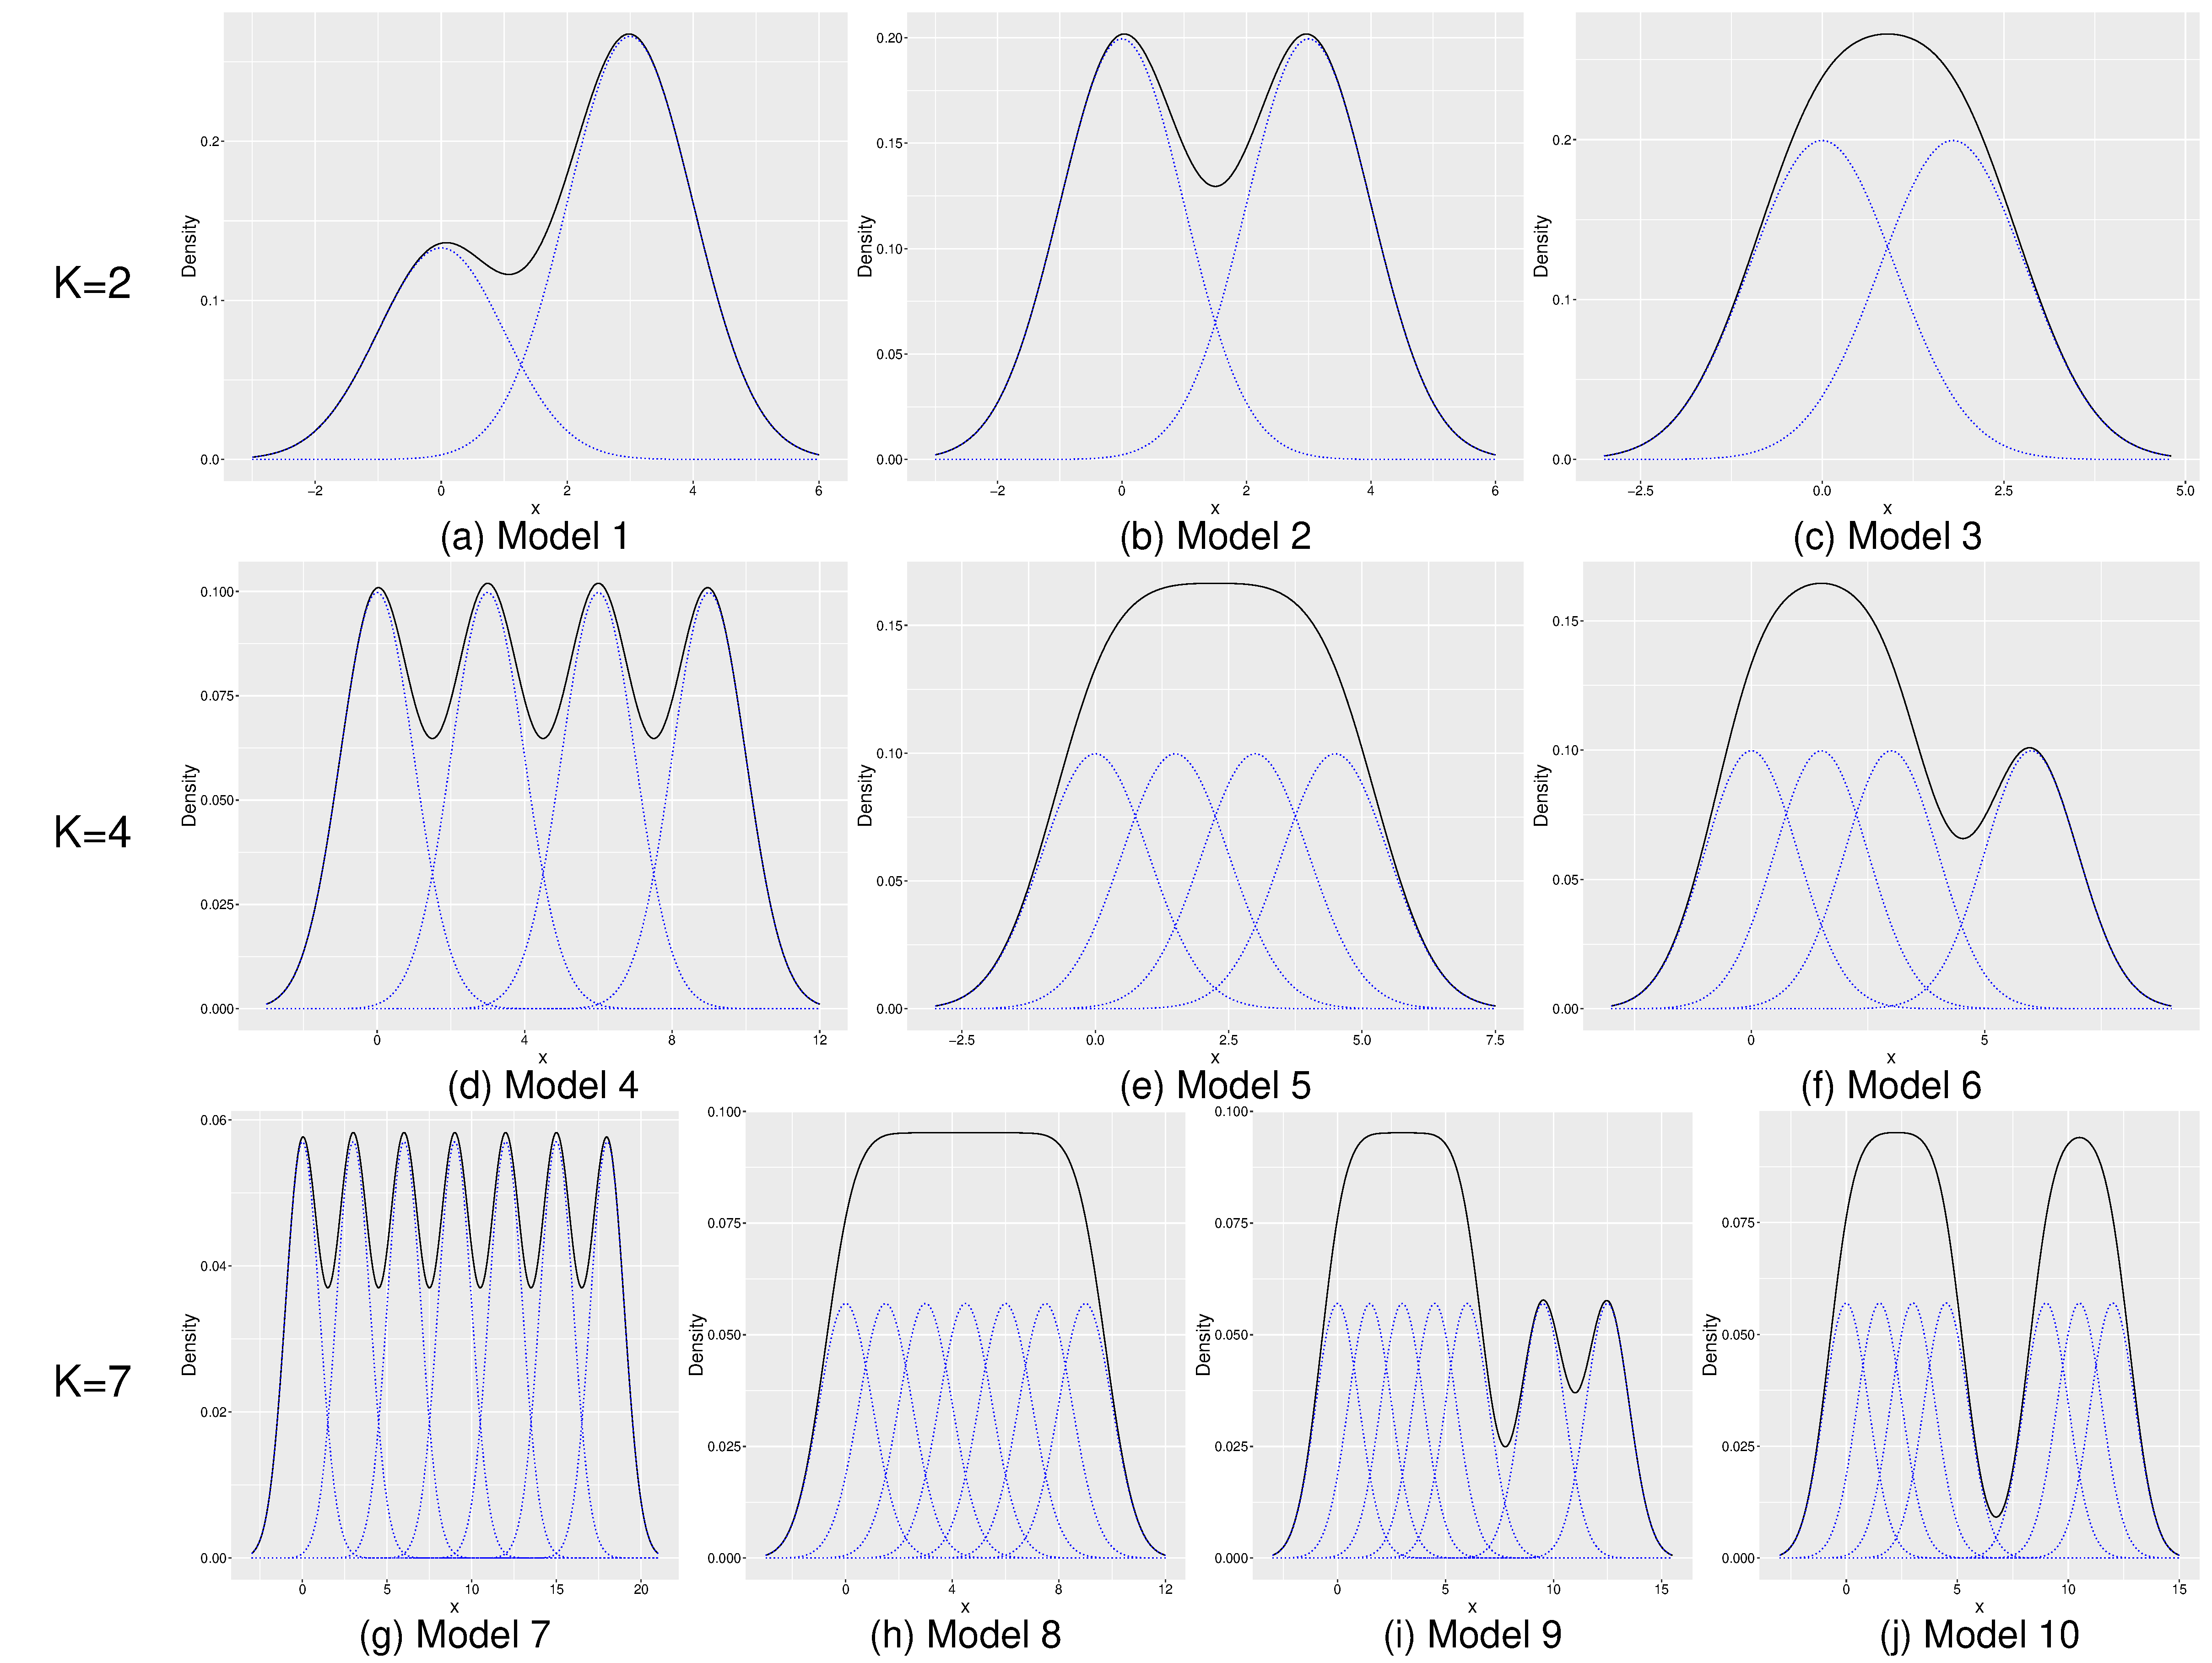
\includegraphics[width = 1\textwidth]{R_Plots_mixture_models_ALL.eps}
%  \captionsetup{font={footnotesize}}   %% 这一句放在 caption前面 %%%%%%%% footnotesize是10pt
%  \caption{高斯混合模型的\wuhao 的密度函数.}
%  \captionsetup{font={small}}   %% 这一句放在 caption前面 %%%%%%%% small是11pt
%  \caption{高斯混合模型的\wuhao 的密度函数.}
%  \captionsetup{font={fivehao}}   %% 这一句放在 caption前面 %%%%%%%% fivehao是前面定义好的10.5pt
%  \caption{高斯混合模型的\wuhao 的密度函数.}
  \captionsetup{font={fivehao}}   %% 这一句放在 caption前面 %%%%%%%% fivehao是前面定义好的10.5pt
  \caption{高斯混合模型的密度函数. 图中实线为混合模型总体的密度函数, 虚线为各成分根据混合比例$\pi_k$放缩后的密度函数.}
  \label{fig:Plot of mixture models} %% label for entire figure
\end{figure}

图\ref{fig:Plot of mixture models}~展示所有高斯混合模型的密度函数. 可以看出, 当且仅当相邻两个成分的均值之差大于$2\sigma$时, 才能在总体密度中直观地区分开来. 参考Ishwaran等(2001), 我们称密度函数中“峰”的个数为众数(mode). 因此, 众数少于成分数的混合模型的参数估计是相对复杂问题.

参考Chen和Khalili~(2008)的做法, 我们对各参数的初始值设定如下: 混合比例$\pi_k^{(0)}=1/K$, 成分均值$\mu_k^{(0)}=100(k-1/2)/K\%$样本分位数($k =1,\cdots,K$). 对于$\sigma$未知的情形, 借鉴Xu和Chen~(2015), 成分标准差被统一设定为上、下四分位数之间的样本标准差. 值得一提的是, 仅EM算法要求设定混合比例的初始值. 在算法的执行过程中, 当$\left\|\bm{\pi}^{(new)}-\bm{\pi}^{(old)}\right\|_1 < 10^{-5}$, $\left\|\bm{\mu}^{(new)}-\bm{\mu}^{(old)}\right\|_1 < 10^{-5}$ 且 $\left\|\bm{\sigma}^{(new)}-\bm{\sigma}^{(old)}\right\|_1 < 10^{-5}$(其中$\left\| \cdot \right\|_1$是$l_1$ 范数)时, 迭代终止, 认为算法已达收敛. 参考Chen和Khalili~(2008), 模型1至模型6采用样本量$n=100$, 而模型7至模型10采用$n=400$.
%CHEN J, KHALILI A. Order selection in finite mixture models with a nonsmooth penalty[J]. Journal of the American Statistical Association, 2008, 103(484):1674-1683.
%XU C, CHEN J. A thresholding algorithm for order selection in finite mixture models[J]. Communications in Statistics - Simulation and Computation, 2015, 44(2):433-453.

表\ref{tab:Algorithm convergence in simulation studies for normal mixture models}~展示了所有算法500次模拟的平均迭代次数及相应的标准差. 从表中可以看出, 无论是收敛速度还是稳定性, 三种改进算法均优于传统的EM算法. 特别地, 在那些众数少于成分数的混合模型中, 新方法达到同样收敛准则的迭代次数仅有EM算法的2\%-33\%. 为了直观地展现该过程, 我们画出了第10个高斯混合模型在$\sigma$未知的情形下, 四种算法的迭代路径, 如图\ref{fig:Iteration paths for the normal mixture model 10 with unknown sigma}~所示. 可以看出, 新方法1、2、3分别需要75、1058、697次迭代, 而EM算法则需要2738次迭代才能达到收敛; 相比传统的EM算法, 本文所提出的新方法的收敛路径变化急剧, 并且需要的迭代次数明显小得多.

\begin{table}[htbp] %"h", "t", "b" and "p" mean "here", "top", "bottom" and "page". Default is "tbp".
%\footnotesize  % setting the size of words in the table (from small to large: \tiny \scriptsize \footnotesize \small \normalsize \large \Large \LARGE \huge \Huge )
\wuhao
\centering
\captionsetup{font={fivehao}}   %% 这一句放在 caption前面 %%%%%%%% fivehao是前面定义好的10.5pt
\caption{各种算法对高斯混合模型进行参所估计的收敛速度.}
\label{tab:Algorithm convergence in simulation studies for normal mixture models}
\medskip
%\begin{tabular}{c c c c cccc}
\begin{tabular}{p{0.74cm}<{\centering} p{0.20cm}<{\centering} p{1.16cm}<{\centering} p{0.74cm}<{\centering} p{2.20cm}<{\centering} p{2.00cm}<{\centering} p{2.20cm}<{\centering} p{2.20cm}<{\centering}}%{c cccccccc c}
%\hline  %p{1.2cm}
\Xhline{1.0pt}
模型 & $n$ & \makecell{成分数} & \makecell{众数} & EM算法 & 新方法1 & 新方法2 & 新方法3 \\
\hline
\multicolumn{8}{c}{方差已知情形} \\%Normal mixture models with known $\sigma^2$
1 & 100 & 2 & 2 & 26.9(8.7) & 15.4(4.9) & 15.9(3.5) & 20.2(5.7) \\
2 & 100 & 2 & 2 & 20.9(6.5) & 11.0(2.9) & 12.3(2.6) & 14.9(3.4) \\
3 & 100 & 2 & 1 & 118.7(93.3) & 14.8(3.1) & 13.1(3.3) & 18.8(4.1) \\
4 & 100 & 4 & 4 & 65.7(55.9) & 31(21.8) & 37.6(16.6) & 53.0(44.2) \\
5 & 100 & 4 & 1 & 829.0(1061.6) & 55.5(40.5) & 140.4(188.7) & 262(355.8) \\
6 & 100 & 4 & 2 & 707.7(1137.1) & 49.3(36.5) & 99.3(86.3) & 214.4(357.9) \\
7 & 400 & 7 & 7 & 88.4(59.7) & 46.6(24.6) & 63.5(22.8) & 79.2(38.7) \\
8 & 400 & 7 & 1 & 2515.6(2802.0) & 148.7(109.8) & 361.3(592.5) & 714.2(659.1) \\
9 & 400 & 7 & 3 & 2172.4(2840.9) & 110.8(86.7) & 201.1(181.2) & 426.1(457.5) \\
10 & 400 & 7 & 2 & 2105.5(2550.7) & 60.6(21.4) & 154.7(126.9) & 263.5(363.9) \\
\multicolumn{8}{c}{方差未知情形} \\%Normal mixture models with unknown $\sigma^2$
1 & 100 & 2 & 2 & 176.2(292.4) & 30.2(25.8) & 35.5(12.4) & 72.8(42.9) \\
2 & 100 & 2 & 2 & 119.6(121.4) & 23.2(13.4) & 29.2(8.6) & 58.5(25.4) \\
3 & 100 & 2 & 1 & 777.7(1313.0) & 26.0(18.4) & 87.1(324.0) & 101.4(263.1) \\
4 & 100 & 4 & 4 & 490.7(703.6) & 44.1(33.4) & 93.7(71.8) & 178.7(131.0) \\
5 & 100 & 4 & 1 & 1186.0(1453.1) & 56.5(38.3) & 173.4(209.3) & 339.9(377.9) \\
6 & 100 & 4 & 2 & 1010.7(1129.3) & 61.3(102.4) & 178.9(210.3) & 294.7(334.8) \\
7 & 400 & 7 & 7 & 2615.6(2527.5) & 71.5(61.7) & 553.9(491.2) & 780.4(812.0) \\
8 & 400 & 7 & 1 & 6025.9(3791.6) & 104.2(71.4) & 1347.4(1575.4) & 1986.8(1787.7) \\
9 & 400 & 7 & 3 & 5401.0(4098.8) & 92.6(64.3) & 956.9(803.0) & 1571.2(1447.2) \\
10 & 400 & 7 & 2 & 5242.1(4132.0) & 99.9(72.6) & 1089.1(1255.2) & 1443.1(1526.6) \\
%\hline
\Xhline{1.0pt}
\end{tabular}
\begin{tablenotes}
  \footnotesize
  \item 注: 众数为模型对应的密度函数图像中“峰”的个数. 圆括号前的数代表500次模拟的平均迭代次数, 圆括号内为相应的标准差.
  %注: 众数为模型对应的密度函数图像中“峰”的个数. 括号前的数代表500次模拟的平均迭代次数, 括号内为相应的标准差. ``CEM''、``New1''、``New2''及``New3'' 分别指经典的EM算法、新方法1、新方法2及新方法3.
  %NOTE: The number before parenthese gives the mean number of iterations, and that in parenthese presents the corresponding standard deviation. ``CEM'', ``New1'', ``New2'' and ``New3'' are the classical EM algorithm, the new method 1, 2 and 3 respectively.
\end{tablenotes}
\end{table}

\begin{figure}[p]
  \centering
  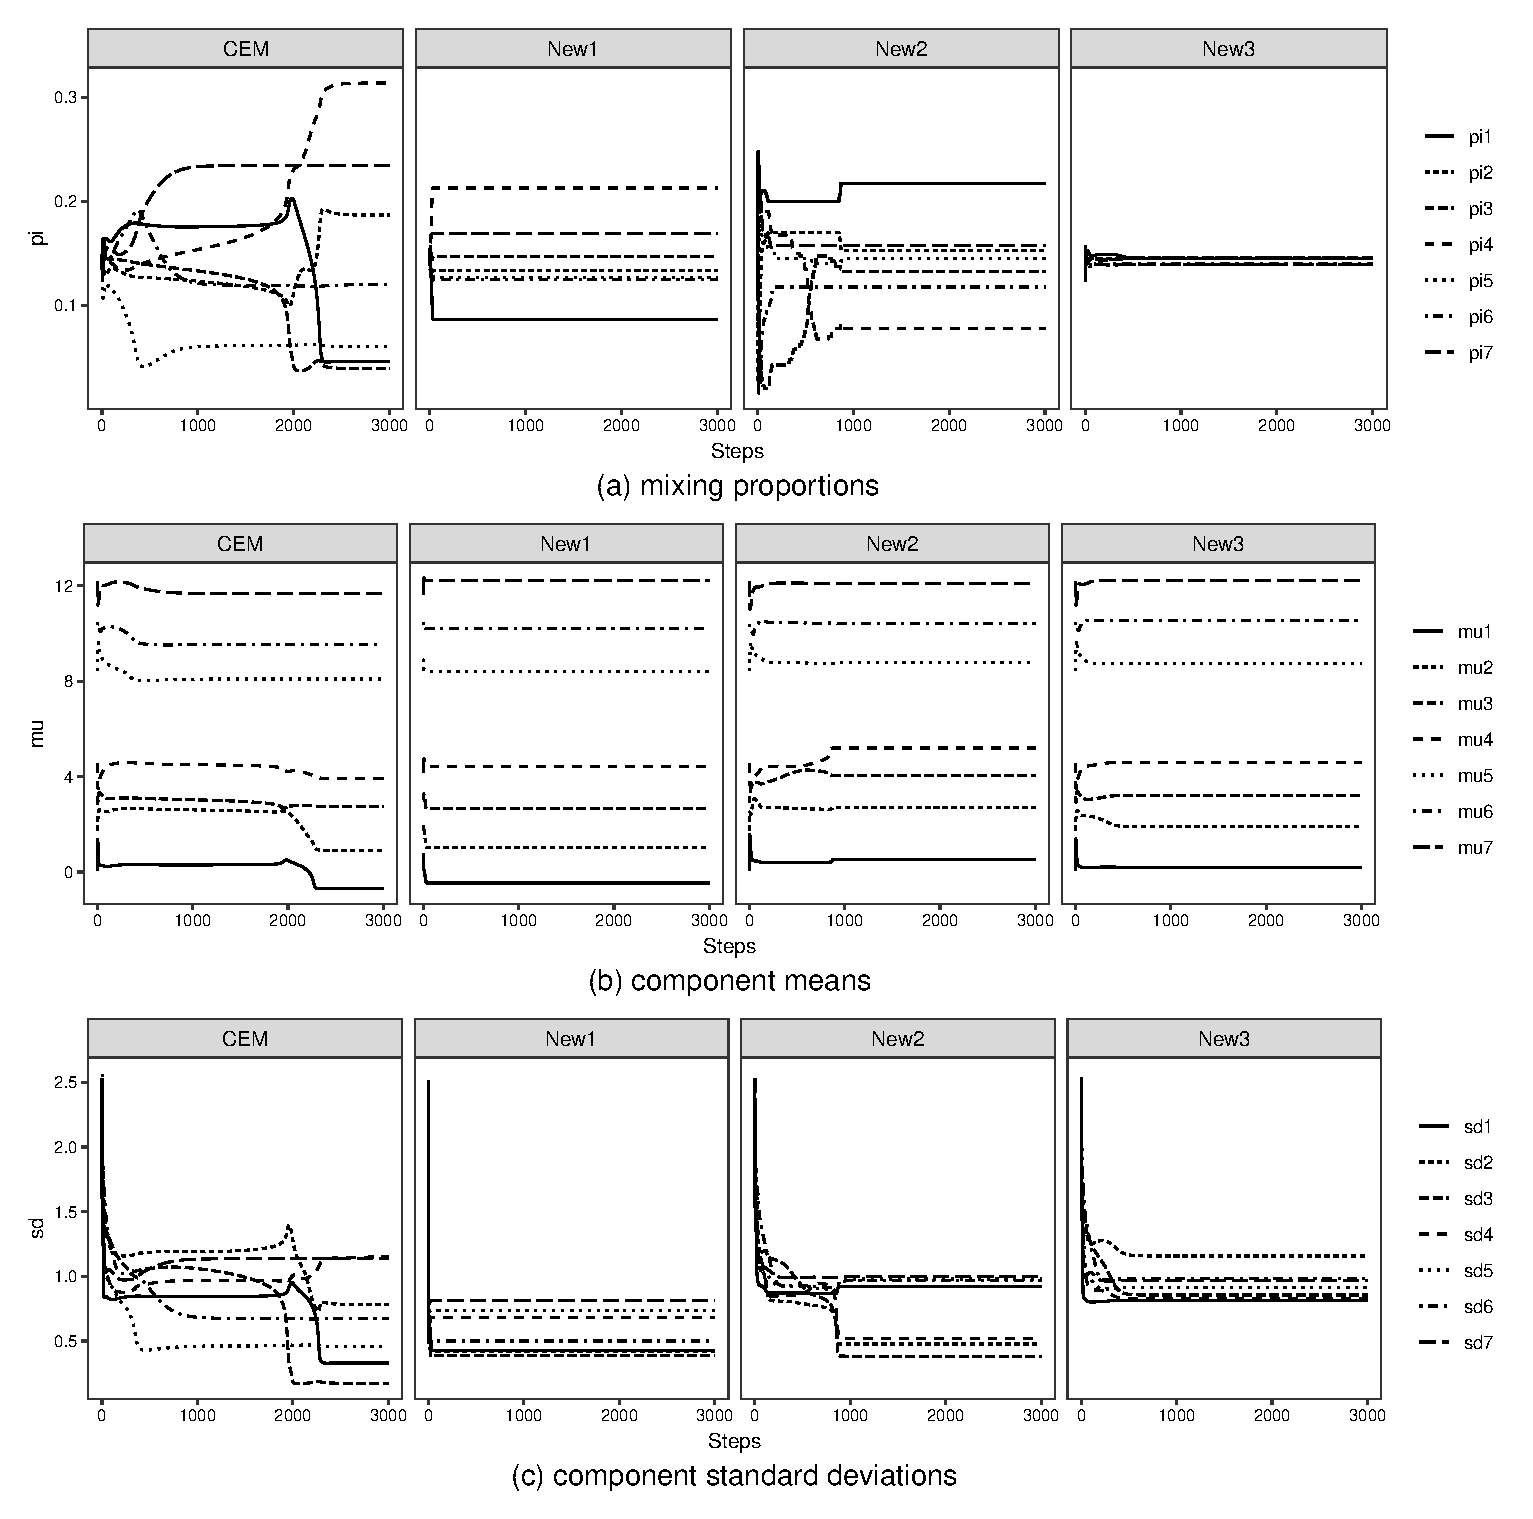
\includegraphics[width = 1\textwidth]{Figure_1_Iteration_paths_for_the_normal_mixture_model_10_with_unknown_sigma.eps}%width = 0.75
  \captionsetup{font={fivehao}}   %% 这一句放在 caption前面 %%%%%%%% fivehao是前面定义好的10.5pt
  \caption{四种算法对七成分高斯混合模型~(表\ref{tab:Parameter values for the normal mixture models}中的模型10)~进行参数估计的迭代路径. 其中``CEM''、``New1''、``New2''及``New3'' 分别指经典的EM算法、新方法1、新方法2及新方法3. 图(a)、(b)、(c)分别是混合比例、成分均值及成分标准差, 且横坐标表示算法的迭代步数, 纵坐标表示参数估计值的大小.}
  \label{fig:Iteration paths for the normal mixture model 10 with unknown sigma} %% label for entire figure
\end{figure}

\begin{figure}[p]
  \centering
  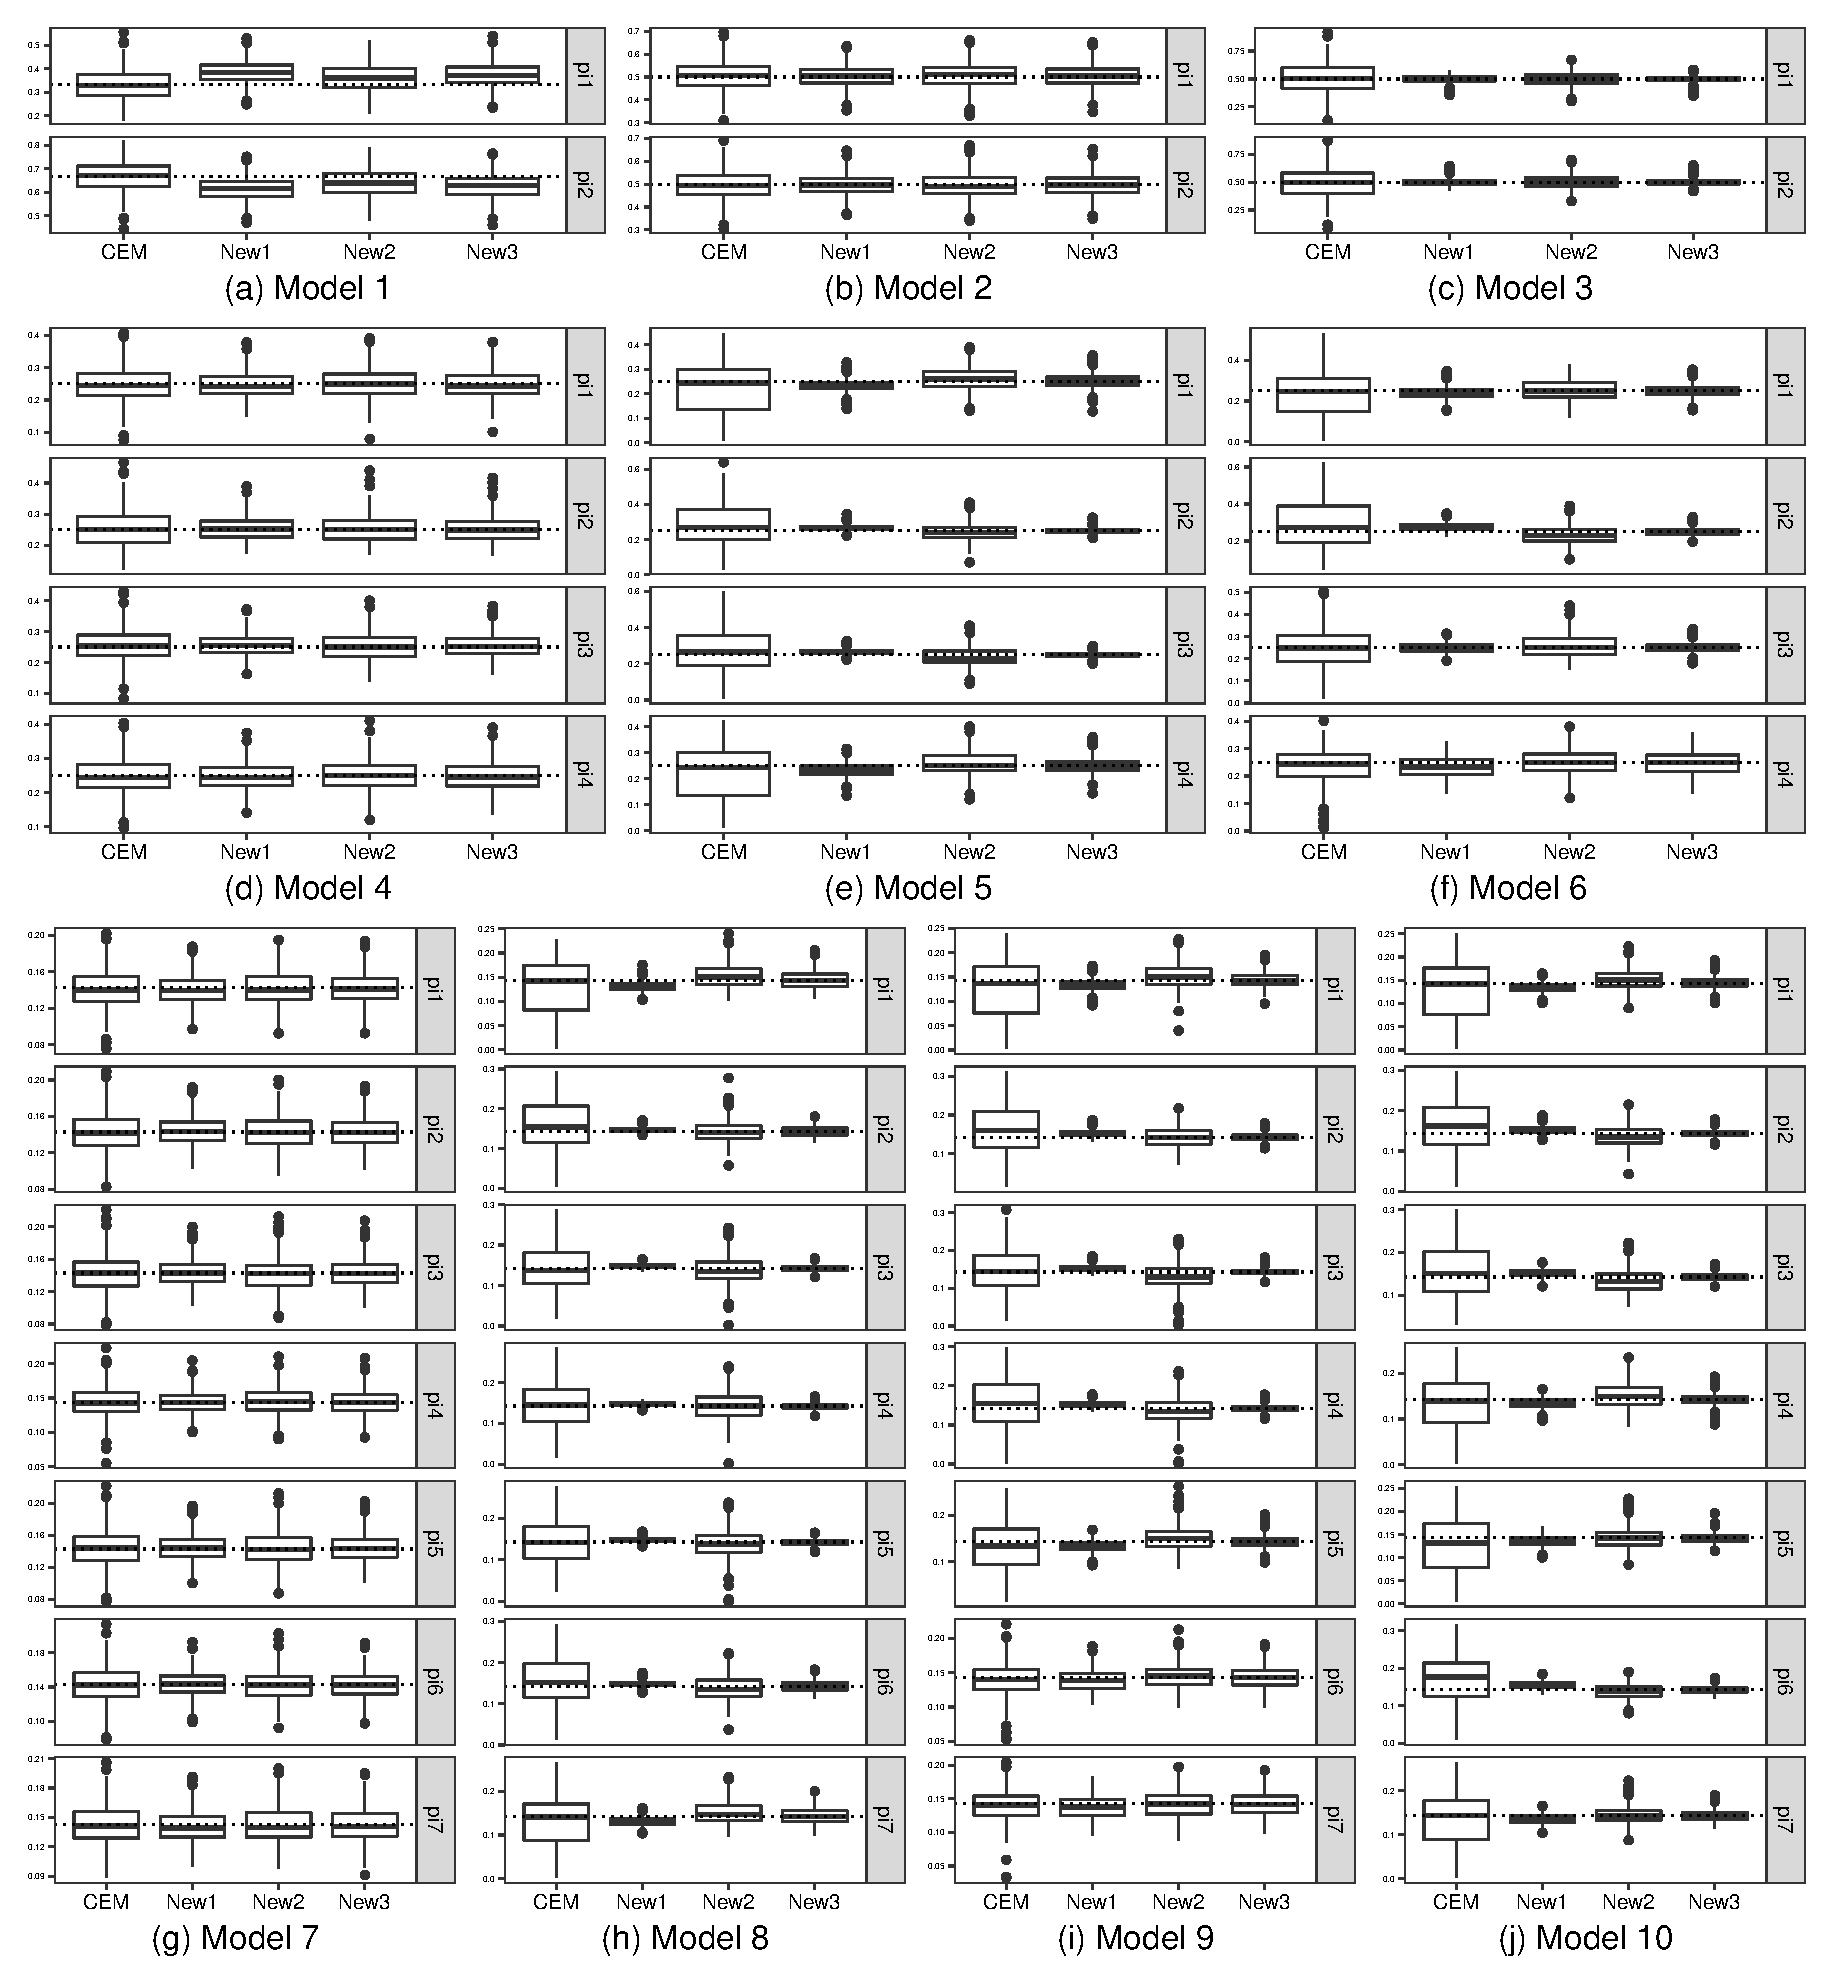
\includegraphics[width = 1\textwidth]{Figure_2_Estimates_for_the_mixing_proportions_for_normal_mixture_models_with_known_sigma.eps}
  \captionsetup{font={fivehao}}   %% 这一句放在 caption前面 %%%%%%%% fivehao是前面定义好的10.5pt
  \caption{方差已知情形下, 各算法对高斯混合模型的混合比例$\pi_k$的估计结果. ``CEM''、``New1''、``New2''及``New3'' 分别指经典的EM算法、新方法1、新方法2及新方法3. 图中虚线表示参数的真实值, 箱形图显示了500次蒙特卡洛模拟的参数估计结果.}
  \label{fig:Estimates for the mixing proportions for normal mixture models 1-10 with known sigma based on 500 replicates} %% label for entire figure
\end{figure}

\begin{figure}[p]
  \centering
  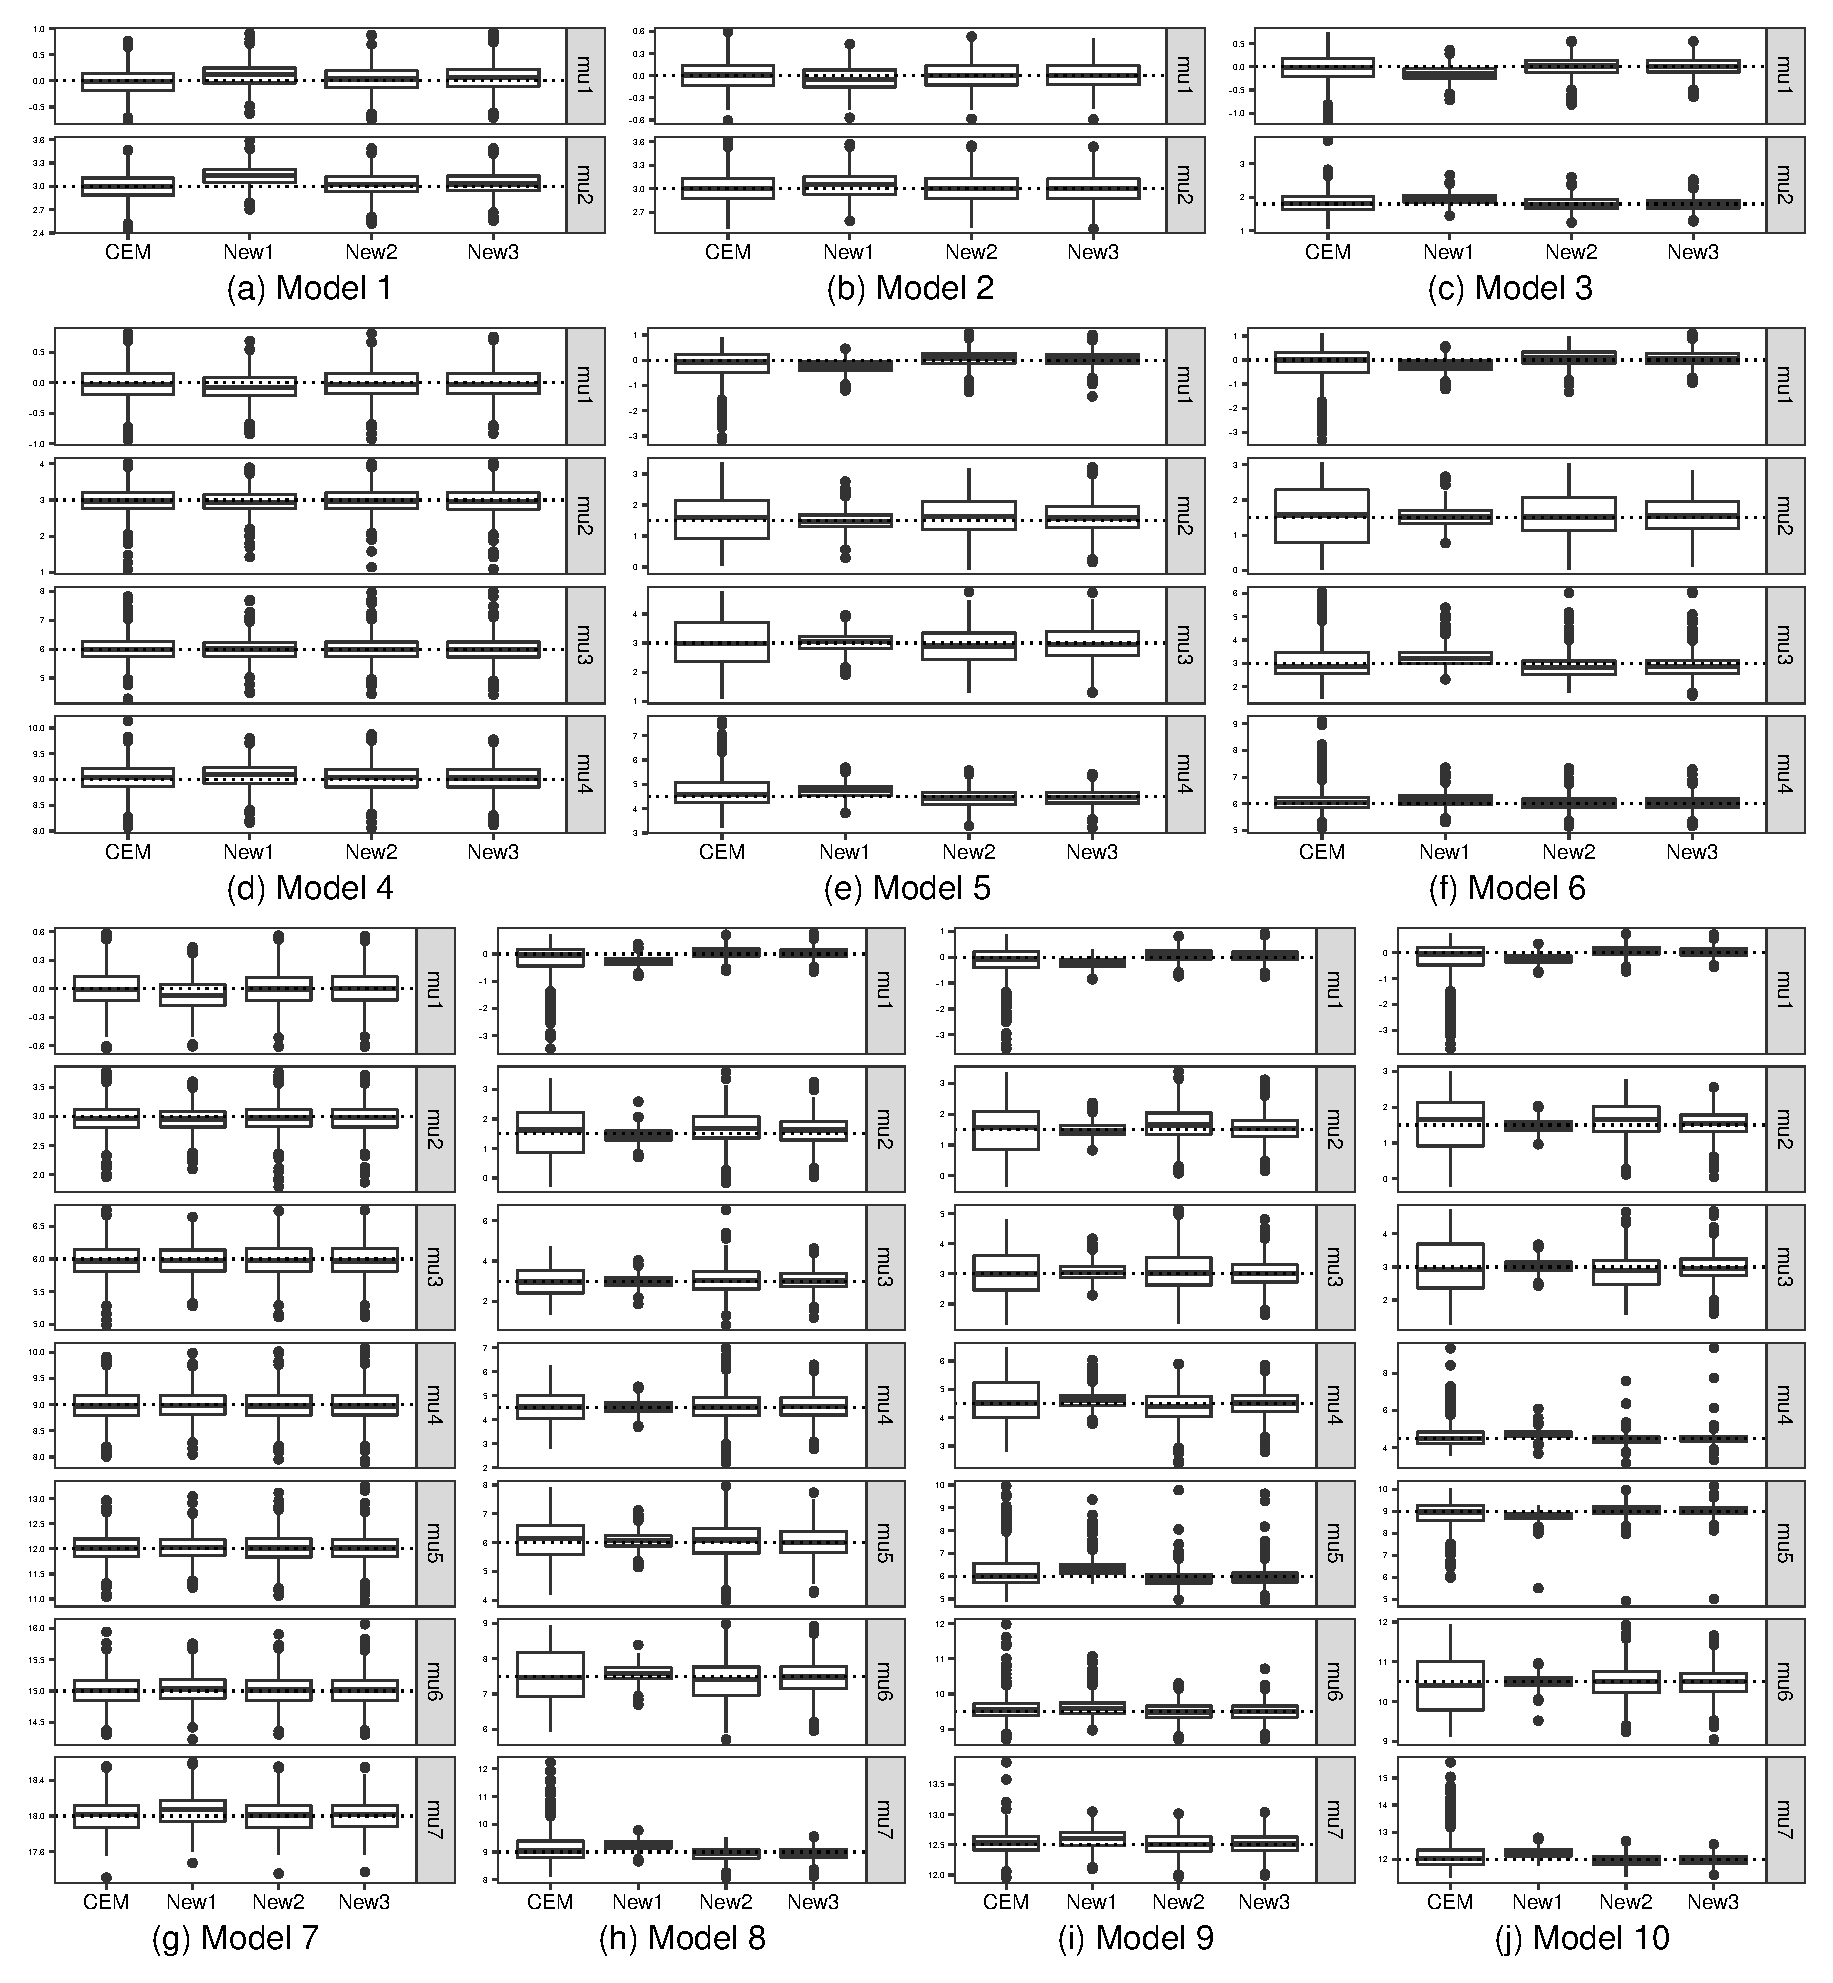
\includegraphics[width = 1\textwidth]{Figure_3_Estimates_for_the_component_means_for_normal_mixture_models_with_known_sigma.eps}
  \captionsetup{font={fivehao}}   %% 这一句放在 caption前面 %%%%%%%% fivehao是前面定义好的10.5pt
  \caption{方差已知情形下, 各算法对高斯混合模型的成分均值$\mu_k$的估计结果.}
  \label{fig:Estimates for the component parameters for normal mixture models 1-10 with known sigma based on 500 replicates} %% label for entire figure
\end{figure}

\begin{figure}[p]
  \centering
  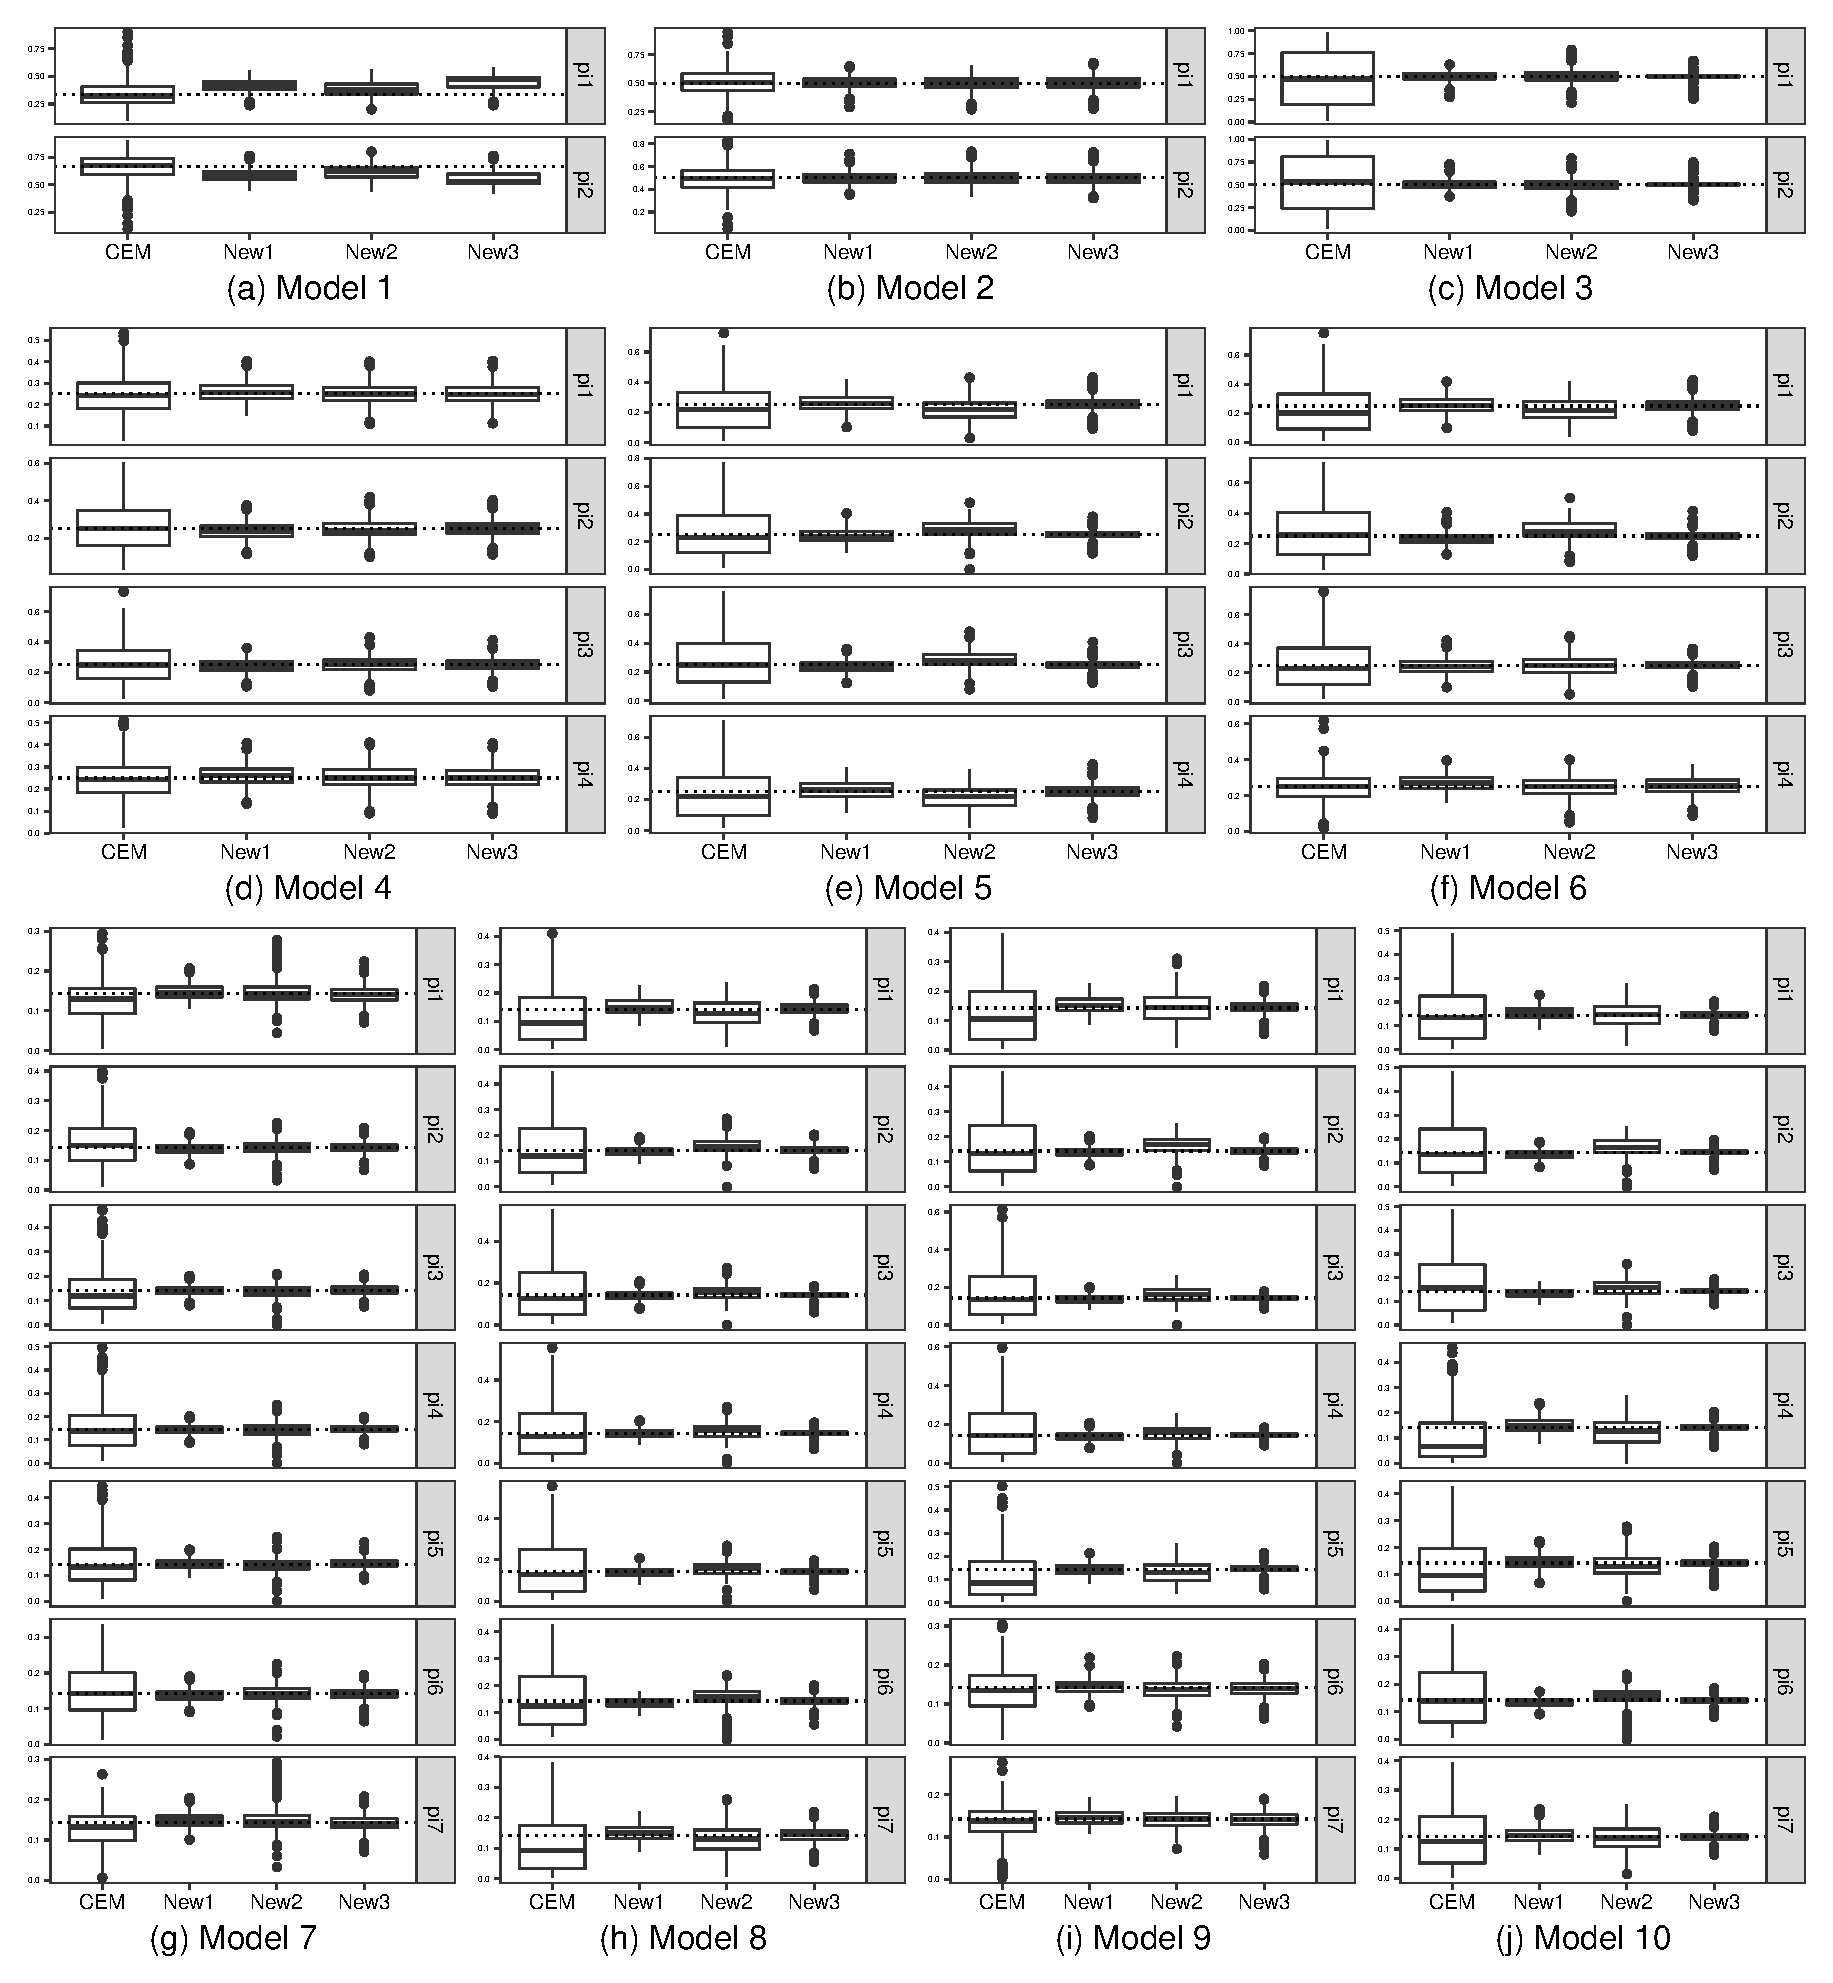
\includegraphics[width = 1\textwidth]{Figure_4_Estimates_for_the_mixing_proportions_for_normal_mixture_models_with_unknown_sigma.eps}
  \captionsetup{font={fivehao}}   %% 这一句放在 caption前面 %%%%%%%% fivehao是前面定义好的10.5pt
  \caption{方差未知情形下, 各算法对高斯混合模型的混合比例$\pi_k$的估计结果.}
  \label{fig:Estimates for the mixing proportions for normal mixture models 1-10 with unknown sigma based on 500 replicates} %% label for entire figure
\end{figure}

\begin{figure}[p]
  \centering
  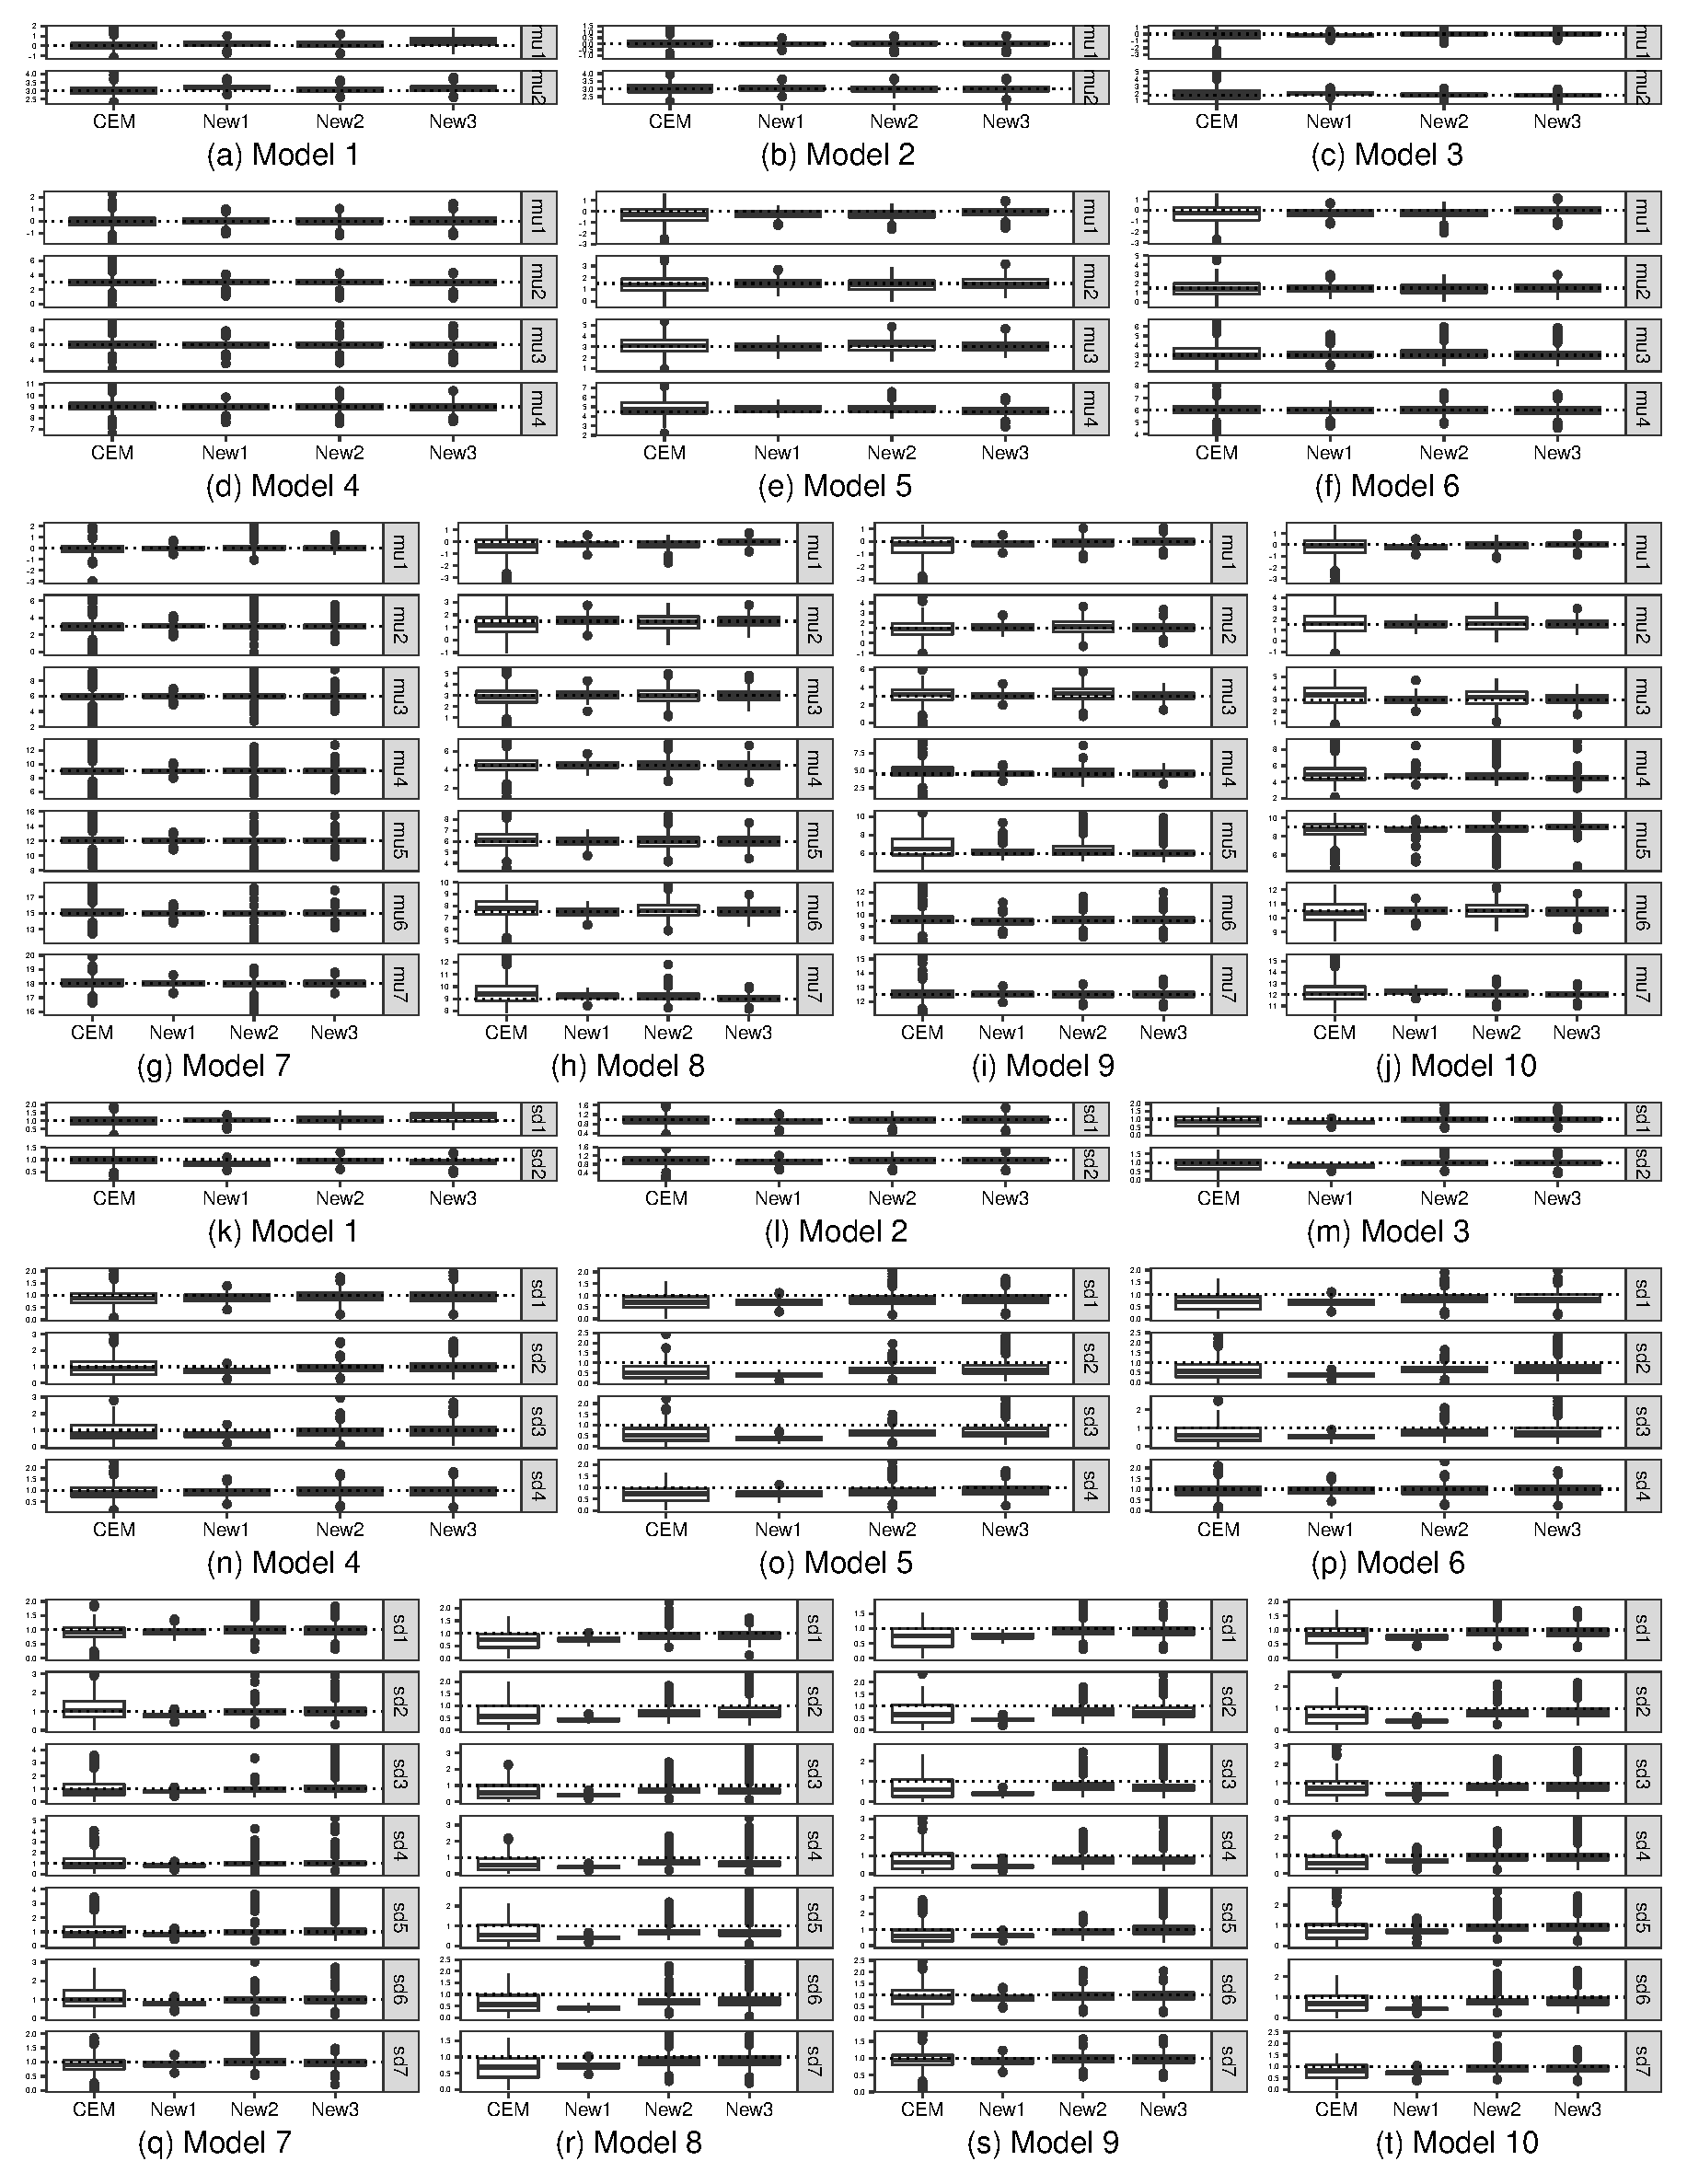
\includegraphics[width = 1\textwidth]{Figure_5_Estimates_for_the_component_parameters_for_normal_mixture_models_with_unknown_sigma.eps}
  \captionsetup{font={fivehao}}   %% 这一句放在 caption前面 %%%%%%%% fivehao是前面定义好的10.5pt
  \caption{方差未知情形下, 各算法对高斯混合模型的成分均值$\mu_k$~((a)-(j))~及成分标准差$\sigma_k$~((k)-(t))~的估计结果.}
  \label{fig:Estimates for the component parameters for normal mixture models 1-10 with unknown sigma based on 500 replicates} %% label for entire figure
\end{figure}

图\ref{fig:Estimates for the mixing proportions for normal mixture models 1-10 with known sigma based on 500 replicates}~至图\ref{fig:Estimates for the component parameters for normal mixture models 1-10 with unknown sigma based on 500 replicates}~展示了各算法对混合比例$\pi_k$及成分参数$\mu_k$、$\sigma_k$的估计情况. 在模型1 中, 传统EM 算法估计效果最好, 但新方法与真实参数值相差不多. 在模型2和模型3中, 所有模型都估计得很好, 其中新方法的估计值方差更小、更加稳定. 在四成分的混合模型, 即模型4至模型6中, 新方法对参数的估计效果明显优于传统EM算法, 特别是在模型众数小于4 的情况(模型5和模型6)下, 优势更显然. 同样地, 在模型7至模型10中, 新方法远远好于EM算法, 并且值得一提的是, 如图\ref{fig:Estimates for the component parameters for normal mixture models 1-10 with unknown sigma based on 500 replicates}(s)和(t)所示, 在第9、第10两个高斯混合模型且$\sigma$ 未知的情形下, 新方法2、3对于成分标准差的估计更靠近真实值, 而EM 算法则偏向于低估该值. 综上不同高斯混合模型的结果, 可以得出结论: 新方法的性能优于传统的EM算法, 特别是在众数小于成分数的复杂混合模型中.

\textbf{\xiaosihao 例~2.2~}
对于泊松混合模型, 其密度函数如下
\begin{equation*}
  g(x; G)=\sum_{k=1}^{K} \pi_{k} \frac{\theta_k^x}{x!} \exp(-\theta_k).
\end{equation*}
我们从Woo和Sriram~(2007)中选取了7个模型. 相应的参数设定可见表\ref{tab:Parameter values for the Poisson mixture models}. 对于每一个模型, 我们均模拟了$n=100, 500$两种不同样本量的情形, 模拟次数同样为500次.
%WOO M J, SRIRAM T. Robust estimation of mixture complexity for count data[J]. Computational Statistics and Data Analysis, 2007, 51(9):4379-4392.

\begin{table}[hp!] %"h", "t", "b" and "p" mean "here", "top", "bottom" and "page". Default is "tbp".
%\scriptsize  % setting the size of words in the table (from small to large: \tiny \scriptsize \footnotesize \small \normalsize \large \Large \LARGE \huge \Huge )
\wuhao
\centering
\captionsetup{font={fivehao}}   %% 这一句放在 caption前面 %%%%%%%% fivehao是前面定义好的10.5pt
\caption{泊松混合模型参数设定.}
\label{tab:Parameter values for the Poisson mixture models}
\medskip
\begin{tabular}{c cccc}
%\hline  %p{1.2cm}
\Xhline{1.0pt}
模型 & ($\pi_1,\theta_1$) & ($\pi_2,\theta_2$) & ($\pi_3,\theta_3$) & ($\pi_4,\theta_4$)\\
\hline
1  & (0.5,1) & (0.5,9)   &          &          \\
2  & (0.8,1) & (0.2,9)   &          &          \\
3  & (0.95,1)& (0.05,10) &          &          \\
4  & (0.45,1)& (0.45,5)  & (0.1,10) &          \\
5  & (1/3,1) & (1/3,5)   & (1/3,10) &          \\
6  & (0.3,1) & (0.4,5)   & (0.25,9) & (0.05,15)\\
7  & (0.25,1)& (0.25,5)  & (0.25,10)& (0.25,15)\\
%\hline
\Xhline{1.0pt}
\end{tabular}
\end{table}

\begin{table}[b!] %"h", "t", "b" and "p" mean "here", "top", "bottom" and "page". Default is "tbp".
%\scriptsize  % setting the size of words in the table (from small to large: \tiny \scriptsize \footnotesize \small \normalsize \large \Large \LARGE \huge \Huge )
\wuhao
\centering
\captionsetup{font={fivehao}}   %% 这一句放在 caption前面 %%%%%%%% fivehao是前面定义好的10.5pt
\caption{各种算法对泊松混合模型进行参所估计的收敛速度.}
\label{tab:Algorithm convergence in simulation studies for Poisson mixture models}
\medskip
\begin{tabular}{c c cccc}
%\hline  %p{1.2cm}
\Xhline{1.0pt}
模型 & $n$ & EM算法 & 新方法1 & 新方法2 & 新方法3 \\
\hline
1 & 100 & 24.2(6.3) & 9.5(1.7) & 11.5(1.3) & 14.7(2.1) \\
 & 500 & 24.1(2.9) & 9.7(0.8) & 11.8(0.6) & 15.1(1.0) \\
2 & 100 & 5.3(1.3) & 2.6(0.6) & 4.8(0.9) & 4.9(1.0) \\
 & 500 & 5.2(0.5) & 2.7(0.5) & 4.9(0.4) & 5.0(0.3) \\
3 & 100 & 27.5(33.6) & 3.8(3.6) & 6.0(1.5) & 6.9(4.0) \\
 & 500 & 20.3(6.1) & 3.0(0.3) & 5.3(0.8) & 6.1(0.8) \\
4 & 100 & 269.2(358.4) & 39.2(24.6) & 56.4(106.6) & 99.4(196.3) \\
 & 500 & 251.5(193.0) & 32.5(13.1) & 30.5(9.9) & 74.8(46.6) \\
5 & 100 & 346.9(439.3) & 43.2(26.2) & 53.6(130.6) & 95.9(100.8) \\
 & 500 & 259.9(156.1) & 40.0(13.9) & 36.8(6.8) & 86.3(35.1) \\
6 & 100 & 628.9(890.6) & 84.6(176.2) & 191.4(428.4) & 289.1(443.2) \\
 & 500 & 1345.1(1518.5) & 56.7(15.1) & 147.6(293.0) & 360.0(475.4) \\
7 & 100 & 869.3(1197.0) & 62.3(34.7) & 115.4(306.2) & 232.9(390.2) \\
 & 500 & 1580.3(1491.7) & 77.5(37.0) & 58.0(30.0) & 178.2(114.1) \\
%\hline
\Xhline{1.0pt}
\end{tabular}
\end{table}

\begin{figure}[htbp]
  \centering
  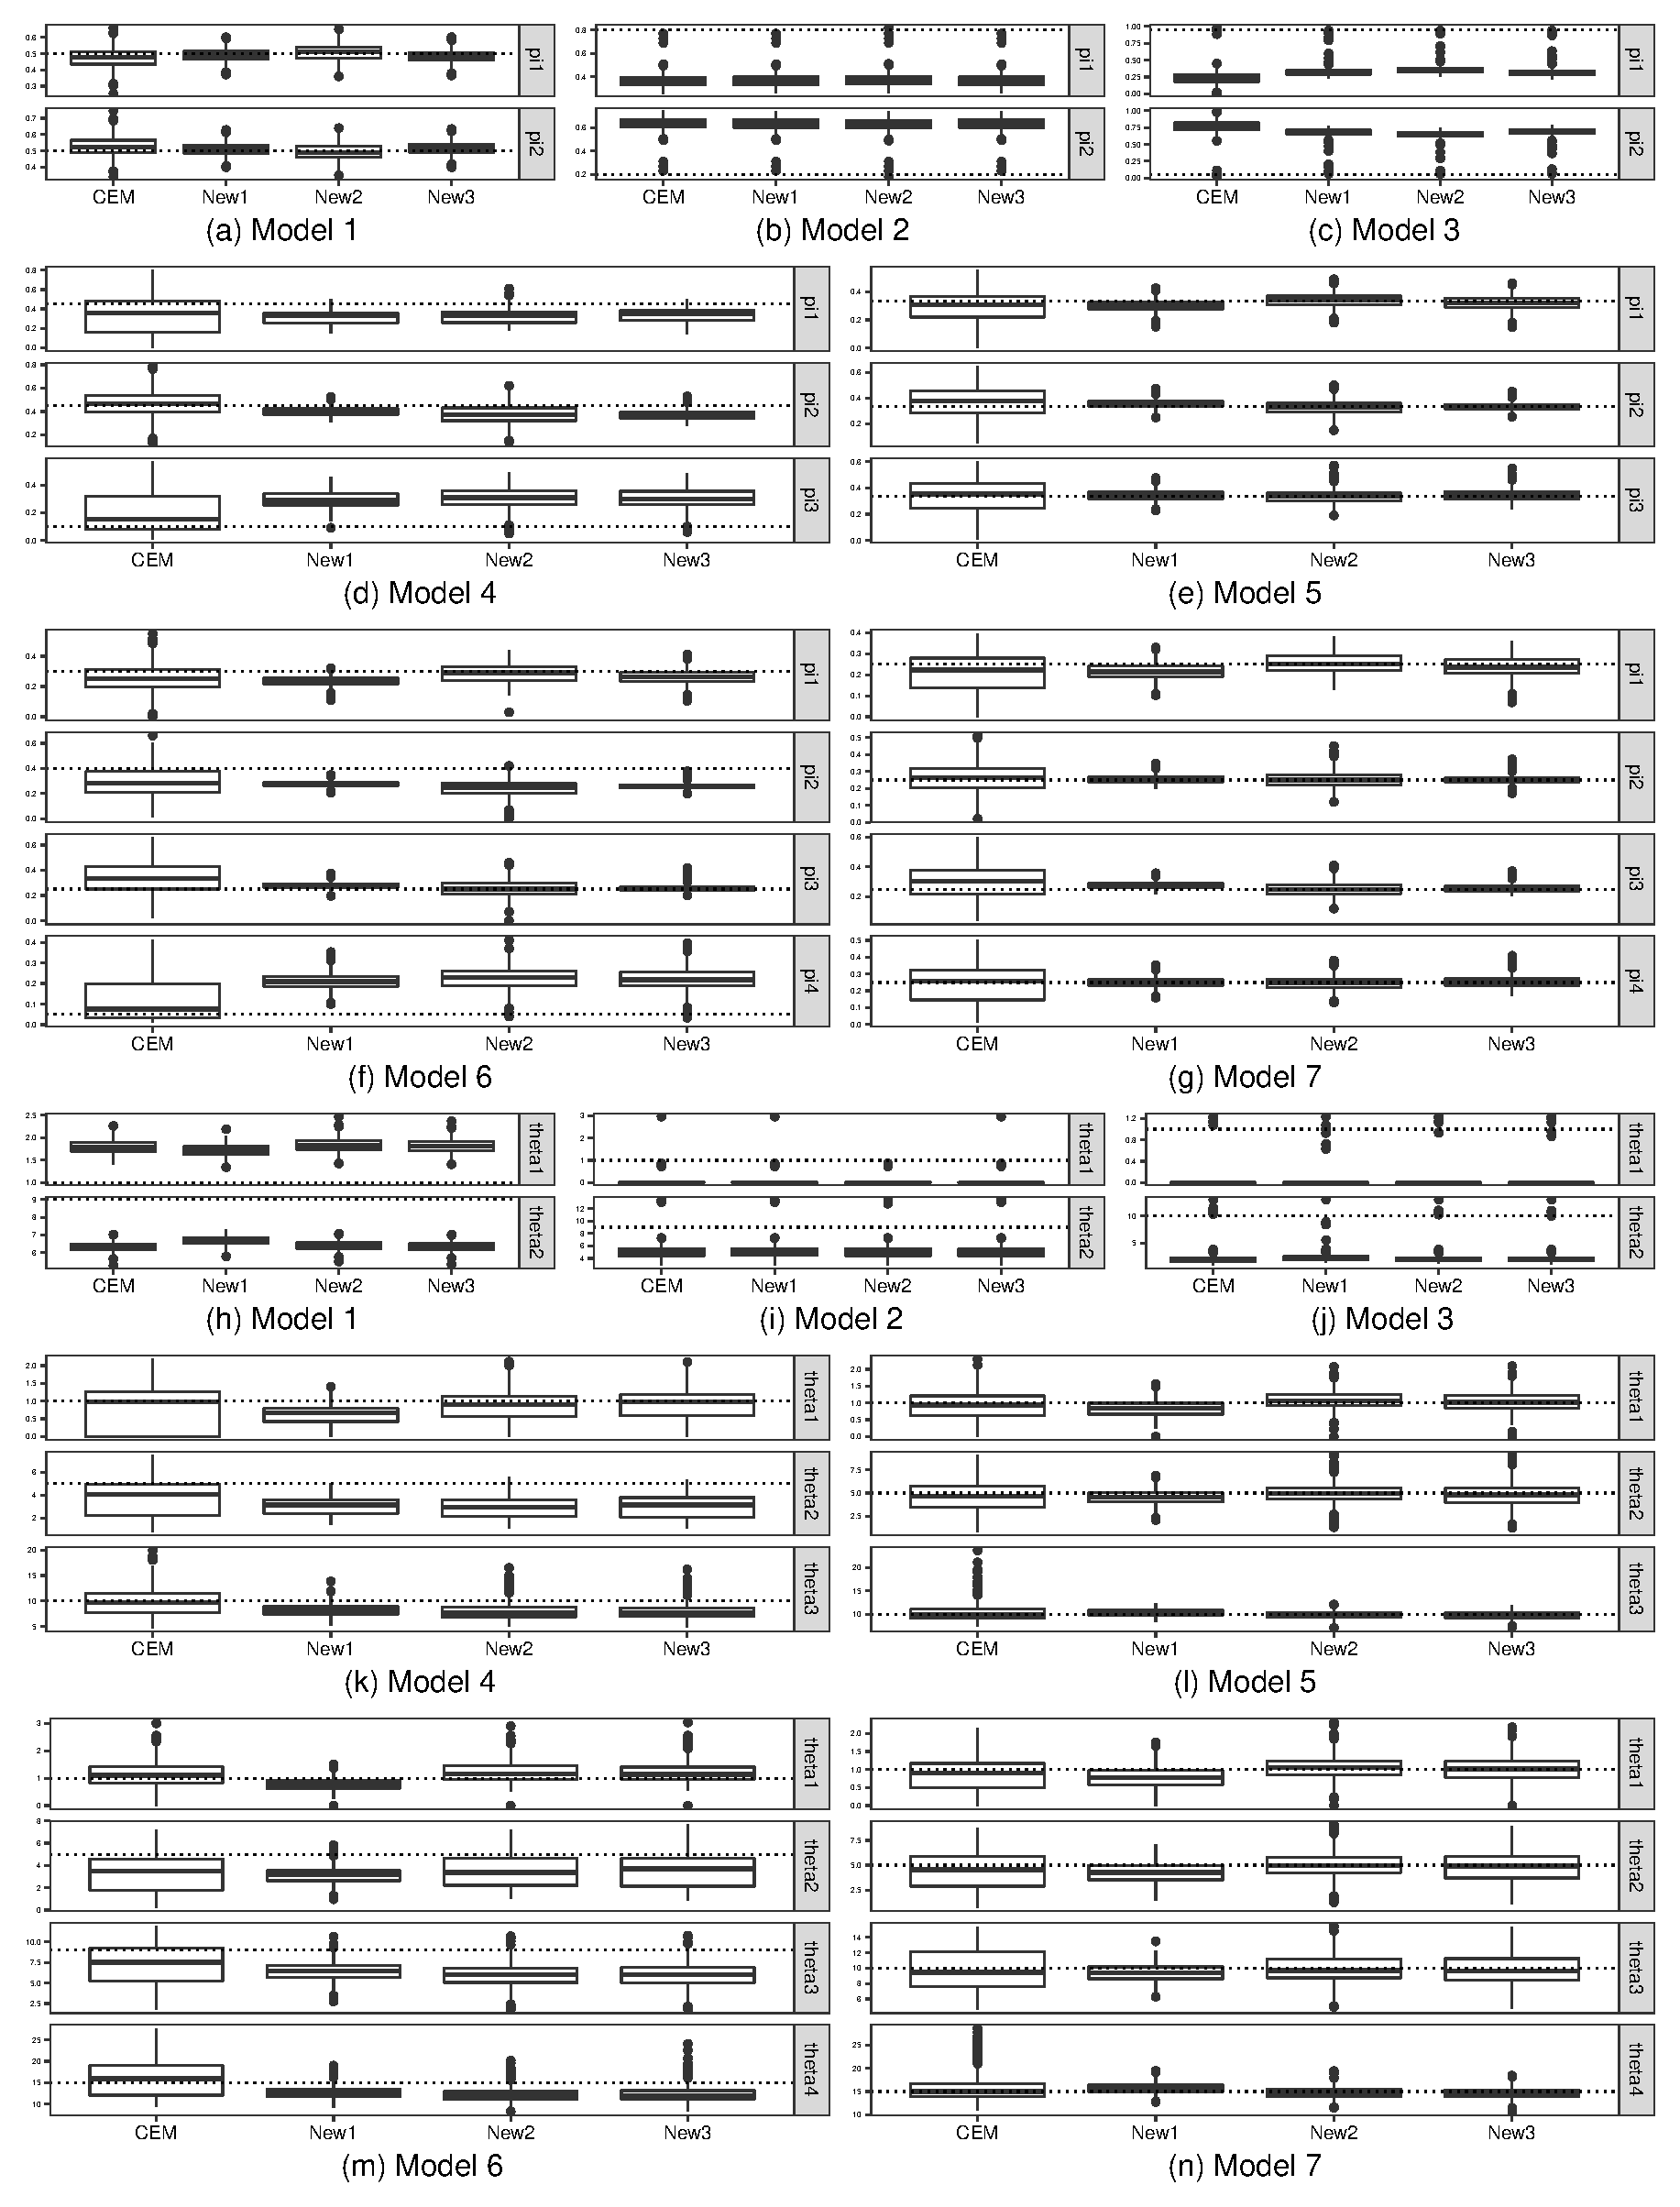
\includegraphics[width = 1\textwidth]{Figure_6_Estimates_for_the_mixing_proportions_and_component_means_for_the_Poisson_mixture_models_with_n_100.eps}
  \captionsetup{font={fivehao}}   %% 这一句放在 caption前面 %%%%%%%% fivehao是前面定义好的10.5pt
  \caption{样本量为100时, 各算法对泊松混合模型的混合比例$\pi_k$~((a)-(g))~及成分参数$\theta_k$~((h)-(n))~的估计结果.}
  \label{fig:Estimates for the mixing proportions and component means for the Poisson mixture models 1-10 with n=100 based on 500 replicates} %% label for entire figure
\end{figure}

\begin{figure}[htbp]
  \centering
  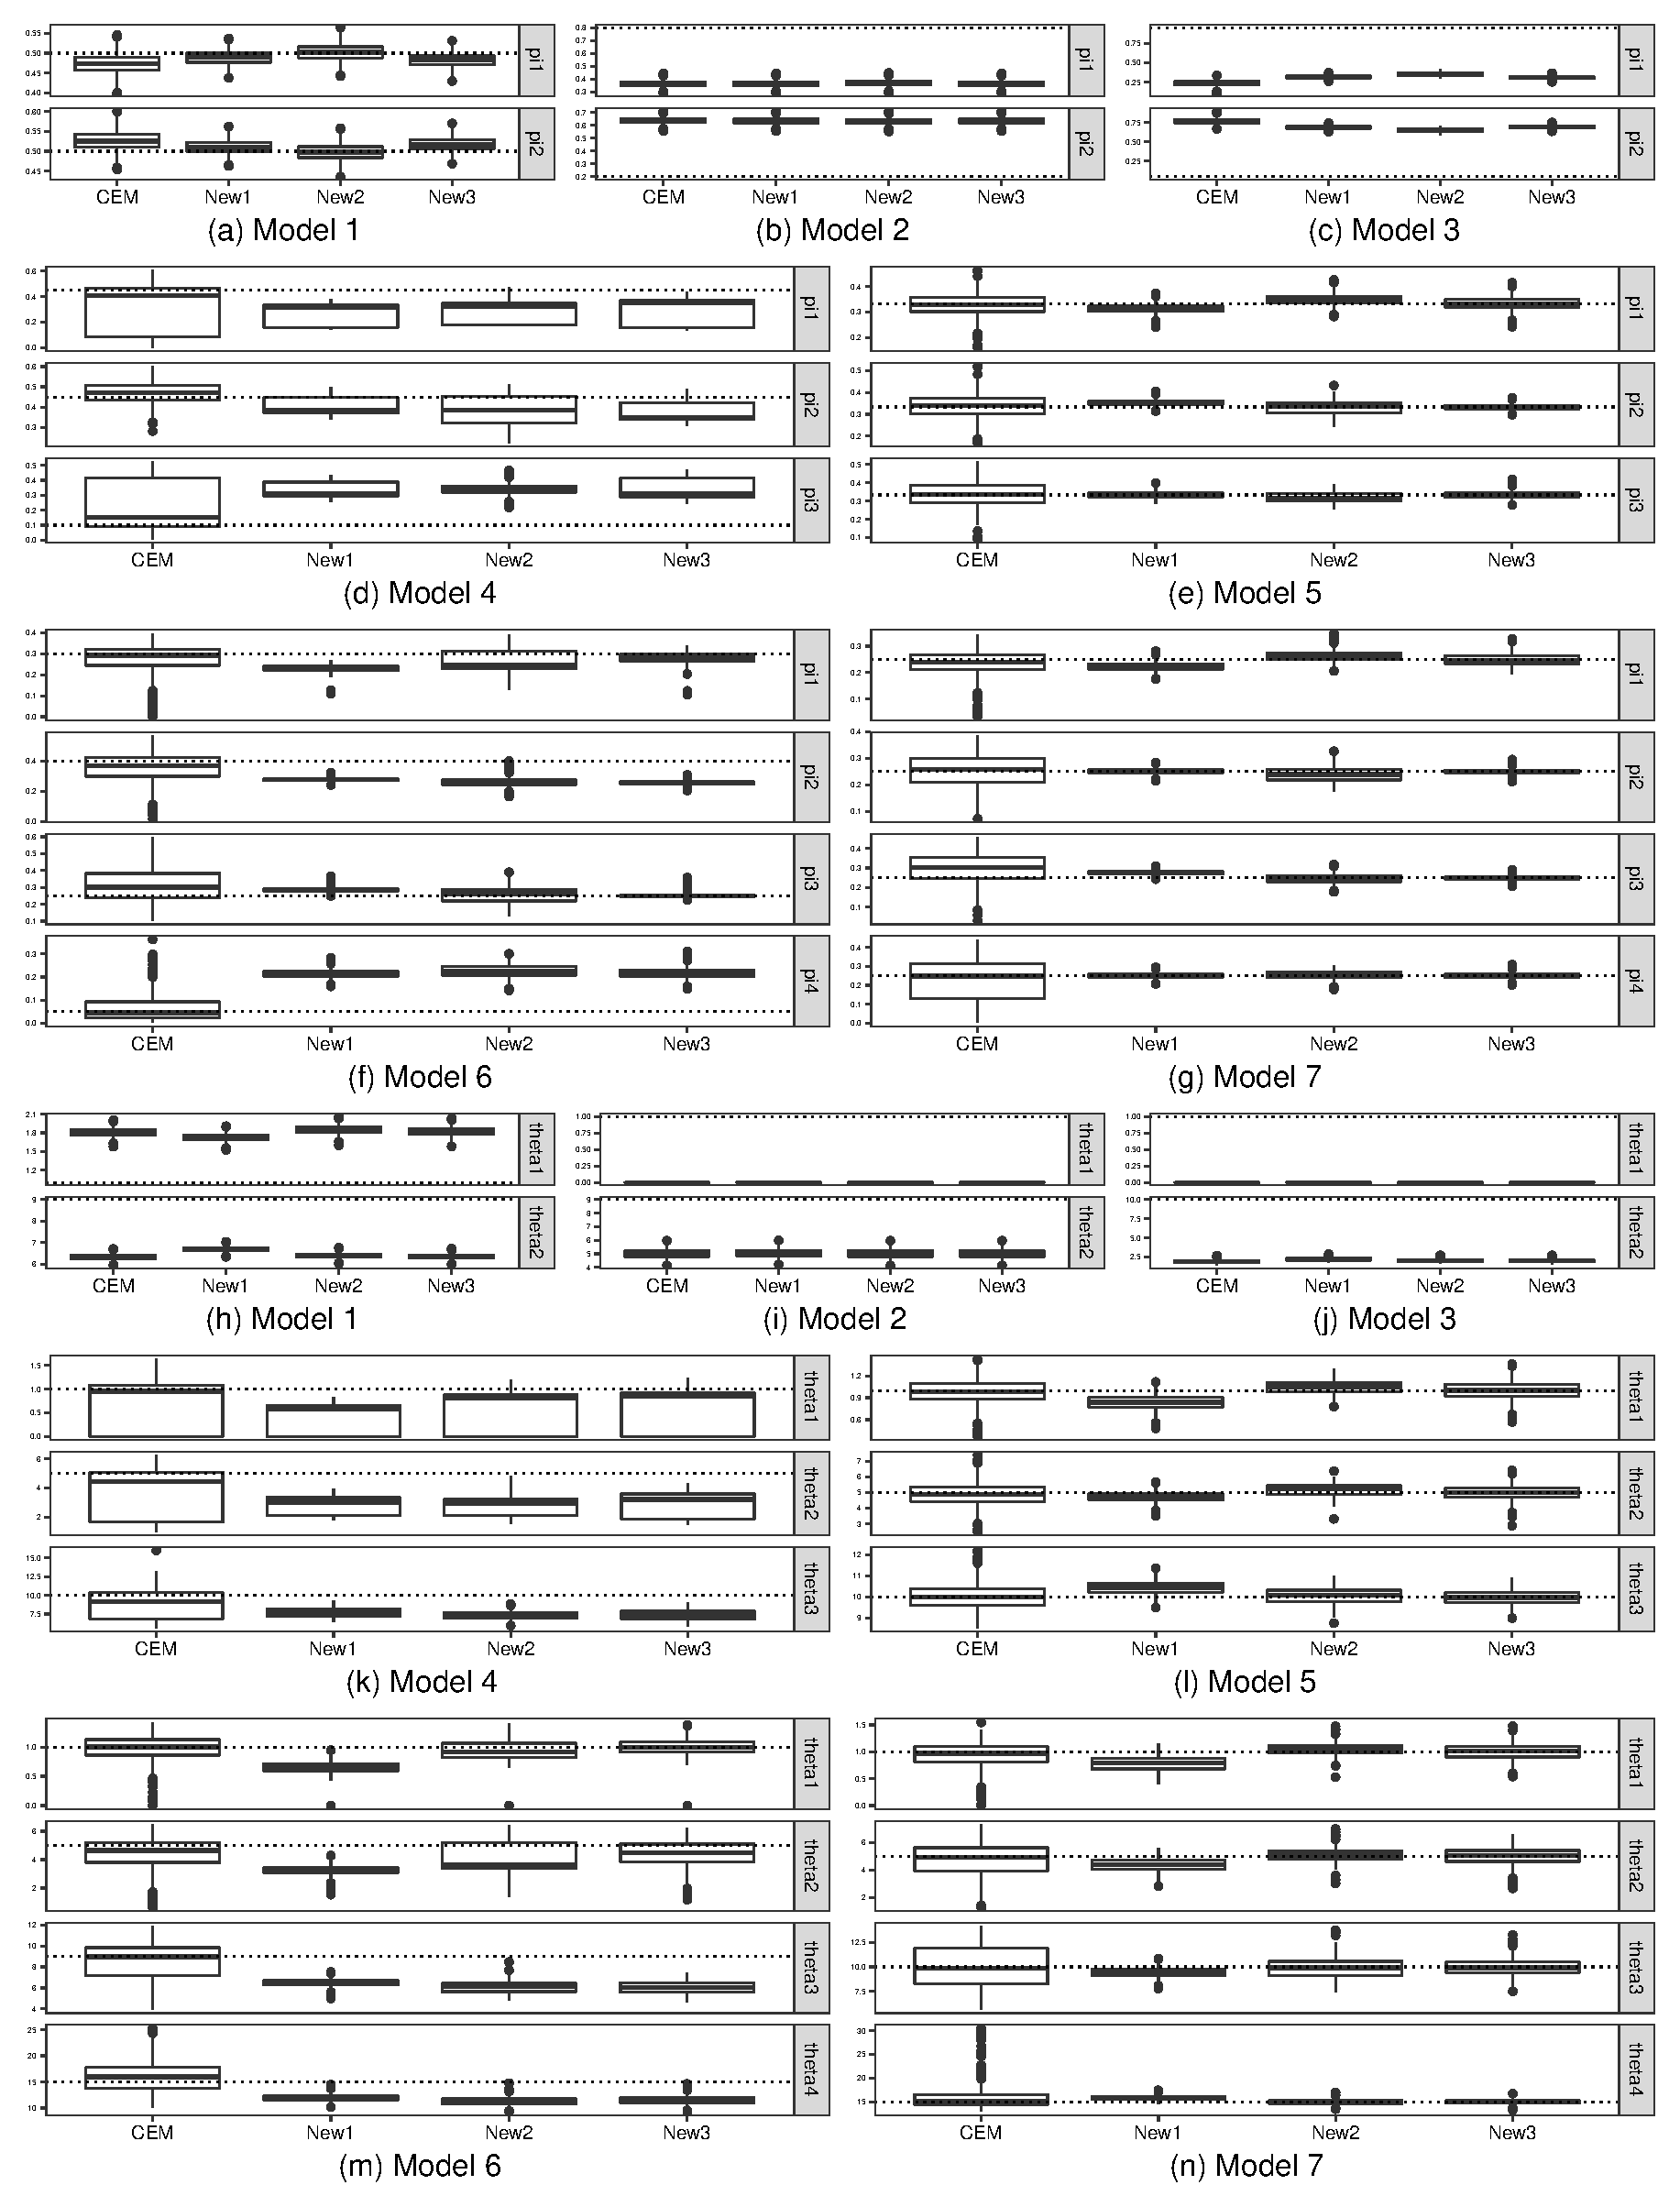
\includegraphics[width = 1\textwidth]{Figure_7_Estimates_for_the_mixing_proportions_and_component_means_for_the_Poisson_mixture_models_with_n_500.eps}
  \captionsetup{font={fivehao}}   %% 这一句放在 caption前面 %%%%%%%% fivehao是前面定义好的10.5pt
  \caption{样本量为500时, 各算法对泊松混合模型的混合比例$\pi_k$~((a)-(g))~及成分参数$\theta_k$~((h)-(n))~的估计结果.}
  \label{fig:Estimates for the mixing proportions and component means for the Poisson mixture models 1-10 with n=500 based on 500 replicates} %% label for entire figure
\end{figure}

表\ref{tab:Algorithm convergence in simulation studies for Poisson mixture models}~展示了各种算法的收敛情况. 从表中可以看出, 随着成分数的增加, 即混合模型越复杂, 新方法的性能较传统EM算法的优势更加明显. 同样地, 箱线图\ref{fig:Estimates for the mixing proportions and component means for the Poisson mixture models 1-10 with n=100 based on 500 replicates}~和\ref{fig:Estimates for the mixing proportions and component means for the Poisson mixture models 1-10 with n=500 based on 500 replicates}~展示了不同方法对混合比例$\pi_k$和成分参数$\theta_k$的估计情况. 在模型1至模型4中, 所有方法的估计效果均不理想, 而在模型5至模型7中, 新方法远远好于传统EM算法的估计效果.

从以上两种模拟例子可以看出, 相比传统的EM算法, 本文所提出的3中新方法明显减少了收敛所需的迭代次数, 特别是在多成分、少众数的复杂混合模型中. 当然, 新方法也存在改进之处, 如上面的泊松混合模型1至模型4中, EM算法和改进的方法均不能取得令人满意的效果.

%\subsubsection{模型的评估}
\subsection{应用实例}
下面我们将改进的EM算法应用到实际数据中.

\textbf{\xiaosihao 例~2.3~}(天文数据集)
我们现研究一个著名的天文数据集. 该数据集包含82个远离银河系的星系移动速度数据(见直方图\ref{fig:Histogram of the galaxy data. The curves show the density of mixture models selected by AIC/BIC based on different algorithms}). 星系移动速度的多模态, 可能意味着由大空隙包围的超星系团的存在, 并且其中的每个模态代表每个星系团以自身的速度移动(Roeder, 1990). 因此, 我们可以用一个带共同成分方差的有限高斯混合分布来对观测数据进行拟合.
%ROEDER K. Density estimation with confidence sets exemplified by superclusters and voids in the galaxies[J]. Journal of the American Statistical Association, 1990, 85(411):617-624.

\begin{figure}[htbp]
  \centering
  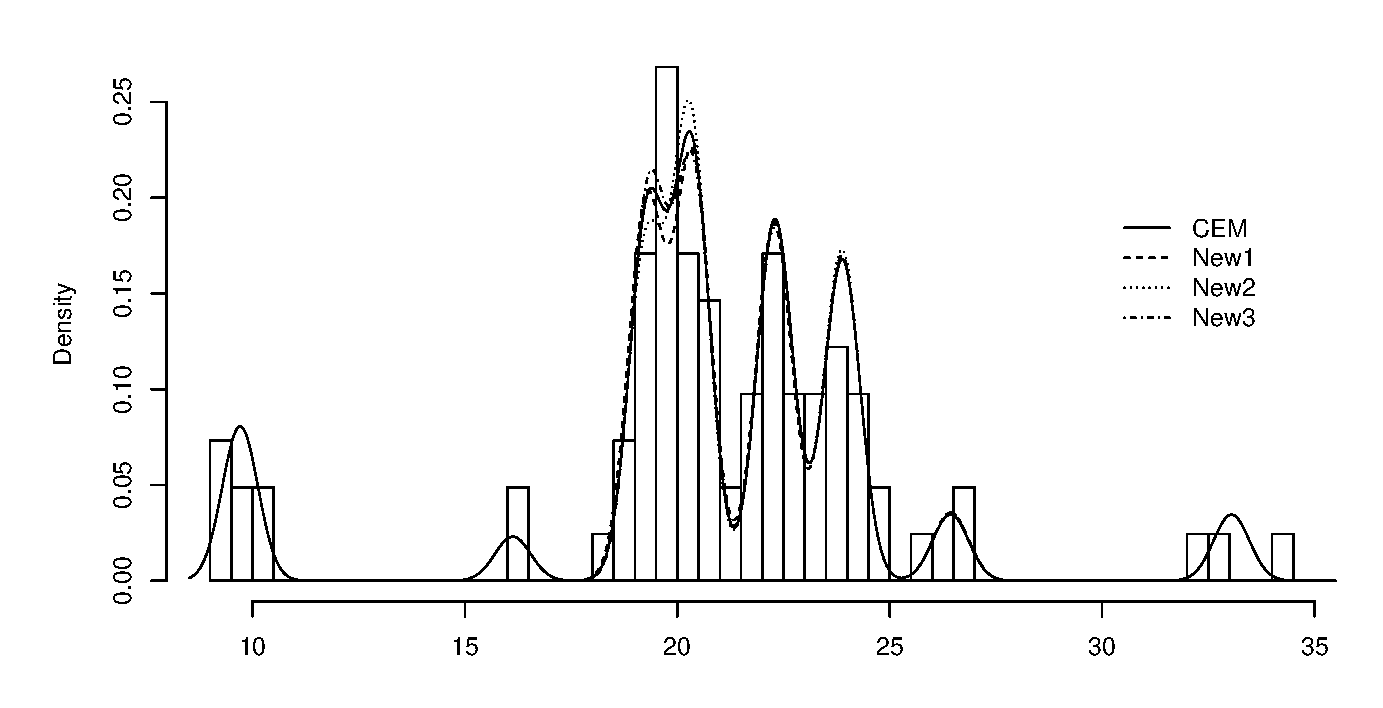
\includegraphics[width = 1\textwidth]{Figure_8_Figure_of_histogram_N_density_in_Example_Postman1986.eps}
  \captionsetup{font={fivehao}}   %% 这一句放在 caption前面 %%%%%%%% fivehao是前面定义好的10.5pt
  \caption{星系数据直方图及模型拟合结果.}
  \label{fig:Histogram of the galaxy data. The curves show the density of mixture models selected by AIC/BIC based on different algorithms} %% label for entire figure
\end{figure}

Richardson和Green~(1997)应用贝叶斯方法, 得出该混合分布的成分数在5到7之间; Xu和Chen~(2015)应用改进的SCAD方法(modified SCAD, MSCAD), 得出该混合分布的成分数为7. 他们的工作不仅证实了数据描述的星系上存在着超星系团, 也为接下来我们的信息准则法(information-based methods)提供成分数的可选范围.
%RICHARDSON S, GREEN P J. On Bayesian analysis of mixtures with an unknown number of components[J]. Journal of the Royal Statistical Society, 1997, 59(4):731-792.
%XU C, CHEN J. A thresholding algorithm for order selection in finite mixture models[J]. Communications in Statistics - Simulation and Computation, 2015, 44(2):433-453.

针对$K=5, 6, \ldots, 11$的每种情形, 我们均利用传统的EM算法及本文所提出的三种改进方法对相应高斯混合分布的参数进行估计, 再利用AIC和BIC两种信息准则法决定$K$的取值. 算法运行的初始值、收敛准则设定同模拟研究一样. 

表~\ref{tab:The outcome of information-based methods for galaxy data}~给出了所有方法的模型结果. 显然, 相比传统的EM算法, 三种改进的方法都只需要更少的迭代次数就能达到收敛(除了方法2中$K=5$的情形以及方法3中$K=7$的情形). 再者, 基于三种改进方法的信息准则均选择了八成分的高斯混合分布作为最终的模型, 模型参数如表~\ref{tab:Parameter estimates for the galaxy data. denote the estimated mixing proportion, component mean, and the common component standard deviation}~所示. 图~\ref{fig:Histogram of the galaxy data. The curves show the density of mixture models selected by AIC/BIC based on different algorithms}~显示, 不同方法对该天文数据的模型分布拟合结果区别不大, 因此改进EM方法的模型精度是可以接受的.

\begin{table}[h!] %"h", "t", "b" and "p" mean "here", "top", "bottom" and "page". Default is "tbp".
%\small   % setting the size of words in the table (from small to large: \tiny \scriptsize \footnotesize \small \normalsize \large \Large \LARGE \huge \Huge )
\wuhao
\centering
\captionsetup{font={fivehao}}   %% 这一句放在 caption前面 %%%%%%%% fivehao是前面定义好的10.5pt
\caption{各算法对星系数据的估计结果.}
\label{tab:The outcome of information-based methods for galaxy data}
\medskip
\begin{tabular}{c cccc cccc}
%\hline  %p{1.2cm}
\Xhline{1.0pt}
\multirow{3}{*}{$K$} & \multicolumn{4}{c}{EM算法} & \multicolumn{4}{c}{新方法1} \\
\cmidrule(lr){2-5} \cmidrule(lr){6-9}
 & 迭代次数 & 对数似然 & AIC & BIC & 迭代次数 & 对数似然 & AIC & BIC \\
\hline
5 & 48 & -321.6 & -335.6 & -352.5 & 21 & -338.9 & -352.9 & -369.8 \\
6 & 20 & -235.8 & -252.8 & -273.3 & 18 & -244.9 & -261.9 & -282.4 \\
7 & 77 & -209.4 & -229.4 & -253.5 & 47 & -222.7 & -242.7 & -266.7 \\
8 & 72 & -198.3 & -221.3 & -249.0 & 27 & -198.4 & -221.4 & -249.1 \\
9 & 106 & -196.6 & -222.6 & -253.8 & 42 & -197.3 & -223.3 & -254.6 \\
10 & 186 & -196.6 & -225.6 & -260.5 & 52 & -197.0 & -226.0 & -260.9 \\
11 & 222 & -193.7 & -225.7 & -264.2 & 57 & -194.5 & -226.5 & -265.0 \\
%\hline
%\hline
\Xhline{1.0pt}
\specialrule{0em}{1pt}{1pt} %https://blog.csdn.net/robert_chen1988/article/details/52695496
%specialrule 命令第一个大括号控制表格线的粗细, 若为0, 则表格线透明, 第二个大括号是表格线与上方内容的距离, 第三个大括号是表格线与下方内容的距离, 通过改变后两个大括号中的值来控制行高!
\Xhline{1.0pt}
\multirow{3}{*}{$K$} & \multicolumn{4}{c}{新方法2} & \multicolumn{4}{c}{新方法3} \\
\cmidrule(lr){2-5} \cmidrule(lr){6-9}
 & 迭代次数 & 对数似然 & AIC & BIC & 迭代次数 & 对数似然 & AIC & BIC \\
\hline
5 & 153 & -321.6 & -335.6 & -352.5 & 40 & -321.6 & -335.6 & -352.5 \\
6 & 18 & -235.8 & -252.8 & -273.3 & 19 & -235.8 & -252.8 & -273.3 \\
7 & 69 & -222.4 & -242.4 & -266.5 & 95 & -222.5 & -242.5 & -266.6 \\
8 & 31 & -198.3 & -221.3 & -249.0 & 42 & -198.3 & -221.3 & -249.0 \\
9 & 40 & -197.3 & -223.3 & -254.6 & 61 & -197.3 & -223.3 & -254.5 \\
10 & 59 & -197.3 & -226.3 & -261.2 & 84 & -196.7 & -225.7 & -260.6 \\
11 & 84 & -194.6 & -226.6 & -265.1 & 105 & -193.9 & -225.9 & -264.4 \\
%\hline
\Xhline{1.0pt}
\end{tabular}
\end{table}

%\begin{table}[ht!] %"h", "t", "b" and "p" mean "here", "top", "bottom" and "page". Default is "tbp".
%%\scriptsize  % setting the size of words in the table (from small to large: \tiny \scriptsize \footnotesize \small \normalsize \large \Large \LARGE \huge \Huge )
%\centering
%\caption{星系数据的参数估计结果. $\hat{\pi}_k$、$\hat{\mu}_k$及$\hat{\sigma}$分别表示混合比例、成分均值及成分标准差($k=1, 2, \ldots, 8$).}
%\label{tab:Parameter estimates for the galaxy data. denote the estimated mixing proportion, component mean, and the common component standard deviation}
%\medskip
%\begin{tabular}{p{0.86cm} p{1.20cm}p{1.40cm}p{1.40cm}p{1.40cm}p{1.40cm}p{1.40cm}p{1.40cm}p{1.40cm} p{0.40cm}}%{c cccccccc c}
%\hline  %p{1.2cm}
%方法 & ($\hat{\pi}_1,\hat{\mu}_1$) & ($\hat{\pi}_2,\hat{\mu}_2$) & ($\hat{\pi}_3,\hat{\mu}_3$) & ($\hat{\pi}_4,\hat{\mu}_4$) & ($\hat{\pi}_5,\hat{\mu}_5$) & ($\hat{\pi}_6,\hat{\mu}_6$) & ($\hat{\pi}_7,\hat{\mu}_7$) & ($\hat{\pi}_8,\hat{\mu}_8$) & $\hat{\sigma}$\\
%\hline
%CEM & (0.09,9.7) & (0.02,16.1) & (0.20,19.3) & (0.24,20.3) & (0.20,22.3) & (0.18,23.9) & (0.04,26.4) & (0.04,33) & 0.42 \\
%New1 & (0.09,9.7) & (0.02,16.1) & (0.21,19.3) & (0.23,20.4) & (0.20,22.3) & (0.18,23.9) & (0.04,26.4) & (0.04,33) & 0.42 \\
%New2 & (0.09,9.7) & (0.02,16.1) & (0.18,19.3) & (0.26,20.3) & (0.20,22.3) & (0.18,23.9) & (0.04,26.4) & (0.04,33) & 0.42 \\
%New3 & (0.09,9.7) & (0.02,16.1) & (0.21,19.3) & (0.23,20.4) & (0.20,22.3) & (0.18,23.9) & (0.04,26.4) & (0.04,33) & 0.42 \\
%\hline
%\end{tabular}
%\end{table}
%%上面这个表格过长了

%%下面我们把它拆分了
\begin{table}[h!] %"h", "t", "b" and "p" mean "here", "top", "bottom" and "page". Default is "tbp".
%\scriptsize  % setting the size of words in the table (from small to large: \tiny \scriptsize \footnotesize \small \normalsize \large \Large \LARGE \huge \Huge )
\wuhao
\centering
\captionsetup{font={fivehao}}   %% 这一句放在 caption前面 %%%%%%%% fivehao是前面定义好的10.5pt
\caption{星系数据的参数估计结果. $\hat{\pi}_k$、$\hat{\mu}_k$及$\hat{\sigma}$分别表示混合比例、成分均值及成分标准差($k=1, 2, \ldots, 8$).}
\label{tab:Parameter estimates for the galaxy data. denote the estimated mixing proportion, component mean, and the common component standard deviation}
\medskip
\begin{tabular}{c ccccc}
%\hline  %p{1.2cm}
\Xhline{1.0pt}
方法 & ($\hat{\pi}_1,\hat{\mu}_1$) & ($\hat{\pi}_2,\hat{\mu}_2$) & ($\hat{\pi}_3,\hat{\mu}_3$) & ($\hat{\pi}_4,\hat{\mu}_4$) & ($\hat{\pi}_5,\hat{\mu}_5$) \\
\hline
EM算法 & (0.09,9.7) & (0.02,16.1) & (0.20,19.3) & (0.24,20.3) & (0.20,22.3) \\
新方法1 & (0.09,9.7) & (0.02,16.1) & (0.21,19.3) & (0.23,20.4) & (0.20,22.3) \\
新方法2 & (0.09,9.7) & (0.02,16.1) & (0.18,19.3) & (0.26,20.3) & (0.20,22.3) \\
新方法3 & (0.09,9.7) & (0.02,16.1) & (0.21,19.3) & (0.23,20.4) & (0.20,22.3) \\
%\hline
\Xhline{1.0pt}
\specialrule{0em}{1pt}{1pt} %https://blog.csdn.net/robert_chen1988/article/details/52695496
%specialrule 命令第一个大括号控制表格线的粗细, 若为0, 则表格线透明, 第二个大括号是表格线与上方内容的距离, 第三个大括号是表格线与下方内容的距离, 通过改变后两个大括号中的值来控制行高!
%\cline{1-5}
\Xcline{1-5}{1.0pt}
方法 & ($\hat{\pi}_6,\hat{\mu}_6$) & ($\hat{\pi}_7,\hat{\mu}_7$) & ($\hat{\pi}_8,\hat{\mu}_8$) & $\hat{\sigma}$ \\
\cline{1-5}
EM算法 & (0.18,23.9) & (0.04,26.4) & (0.04,33) & 0.42 \\
新方法1 & (0.18,23.9) & (0.04,26.4) & (0.04,33) & 0.42 \\
新方法2 & (0.18,23.9) & (0.04,26.4) & (0.04,33) & 0.42 \\
新方法3 & (0.18,23.9) & (0.04,26.4) & (0.04,33) & 0.42 \\
%\cline{1-5}
\Xcline{1-5}{1.0pt}
\end{tabular}
\end{table}

%\subsubsection{数据介绍}
\section{小结}
本章研究了有限混合模型的参数估计问题. 首先, 我们介绍了经典EM算法在混合模型参数估计中的应用, 以及算法收敛速度慢的问题. 接着, 我们对E步中隐变量条件期望的计算方法进行修改, 提出了三种改进的EM算法: 第一种改进算法视上一次迭代的参数估计结果为先验信息, 将每个样本所属各个成分的可能性作为其混合比例的新估计值; 第二种改进算法的思想来源于有限混合模型的抽样过程. 我们根据每一次迭代后的参数估计值对样本进行分类, 用各个成分的样本比率来替换混合比例; 第三种改进算法将第一种算法中每个样本所属各个成分的可能性作平均, 得到混合比例的新估计值. 新算法和经典EM算法一样都具有收敛性, 但由于每一次迭代时, 新算法都会利用样本信息, 因此加快了收敛速度, 这在本章最后的模拟研究及实例应用中都得到了印证. 同时, 数值试验结果也展示了新算法对有限混合模型的参数估计效果更准确和稳定.

值得一提的是, 本章所展示的有限混合分布是一元的, 但无需额外工作量, 便可拓展到多元情形.
%随机变量$x$

\chapter[基于MMCP方法的有限混合模型定阶研究]{基于MMCP方法的有限混合模型定阶研究}
本章将研究另一个问题, 有限混合模型的定阶. 由于所提出的新方法是在AIC、BIC等信息准则方法的基础上进行改动的, 因此我们首先在本章第1节中介绍相关工作, 其次在第2节中介绍新方法及其数值求解算法, 最后在第3节中用实验数据验证所提出MMCP方法的效果.

\section{相关工作}
\label{sec:related work on order selection}
\subsection{基于信息准则法的有限混合模型定阶}
AIC~(Akaike, 1973)和BIC~(Schwarz, 1978)是最常见的两种模型选择方法. Leroux~(1992)将AIC和BIC应用到有限混合模型的定阶问题中.
%AKAIKE H. Information theory and an extention of the maximum likelihood principle[C]//Second International Symposium on Information Theory,(1973). 1973: 267-281.
%SCHWARZ G. Estimating the dimension of a model[J]. The Annals of Statistics, 1978, 6(2):461-464.
%LEROUX B G. Consistent estimation of a mixing distribution[J]. The Annals of Statistics, 1992: 1350-1360.

假定有来自某有限混合分布的一组独立随机样本, 记对数似然函数为$l_{n}(G)$. AIC信息被定义为备选模型中参数个数的函数. 在有限混合模型中, 参数的个数与阶$K$成正比, 因此有
\begin{equation*}
  AIC(K)=l_{n}(\hat{G})-a_K,
\end{equation*}
式中$\hat{G}$是$K$成分混合模型的参数$G$的极大似然估计, $a_K$是$K$成分混合模型中的参数总个数.

BIC信息与AIC信息的表达式只有稍微不同, 为
\begin{equation*}
  BIC(K)=l_{n}(\hat{G})-\frac{1}{2}(\log{n})a_K,
\end{equation*}
式中$n$为样本个数. 
 
在实际中, 我们需要在一个较大的参数空间~(如[0, 2$K_0$], 其中$K_0$为真实的成分个数)~中计算每一个$K$取值下的信息量, 最后取AIC或BIC最大时的$K$作为模型阶的估计. 由于AIC及BIC不是关于参数个数的单调递增函数, 因此所得到的模型在一定程度上能够防止过拟合. 但由于这两种方法都需要在一个较大的参数空间上进行搜索, 特别是当模型很复杂($K_0$很大)时, 需要消耗大量的计算时间.

\subsection{基于惩罚最小距离法的有限混合模型定阶}
Chen和Kalbfleisch~(1996)在AIC及BIC的思想上, 提出了惩罚最小距离法(penalized minimum-distance criterion). 信息准则法直接对模型参数的个数进行惩罚, 而惩罚最小距离法则是对混合比例进行惩罚. 给定一有限混合模型的随机独立样本$\{x_1, x_2, \cdots, x_n\}$, 并假设其累计分布函数为
%CHEN J, KALBFLEISCH J D. Penalized minimum‐distance estimates in finite mixture models[J]. Canadian Journal of Statistics, 1996, 24(2):167-175.
\begin{equation*}
  C(x; G)=\sum_{k=1}^{K}\pi_{k}F(x, \theta_{k}).
\end{equation*}
记经验分布函数为$F_{n}(x)=\frac{1}{n}\sum_{i=1}^{n}I(x_{i} \leq x)$; $d(F_{n}(x), C(x; G))$表示$F_{n}(x)$和$C(x; G)$两个函数之间的距离(如kolmogrov-Smirnov距离、Cramer-VonMises距离).

惩罚最小距离法中的距离函数为
\begin{equation}
\label{equ:penalized distance in penalized minimum-distance criterion}
  D(F_{n}(x), C(x; G))=d(F_{n}(x), C(x; G))-C_{K}\sum_{k=1}^{K}\log\pi_{k},
\end{equation}
其中$C_{K}>0$为可调参数. 由上式可以看出, 如果某些$\pi_{k}$过小, 那么该距离函数的值就会很大, 因此该方法能够防止$K$估计值较大引起的过拟合情况, 然而, 该方法的计算程序和信息准则法一样, 需要在一个较大的参数空间里计算成分数$K$的所有可能取值对应的距离函数值, 再进行比较之后得出结论. 再者, 基于惩罚最小距离法对有限混合模型依旧不能防止另一种过拟合情况: 混合模型中存在相近成分, 即某些子群体的参数差别不大, 我们将在章节\ref{sec:theory and algorithm to MMCP}~中具体研究这种过拟合情况并提出相应的解决方法.

\subsection{回归模型中的变量选择}
考虑线性回归模型
\begin{equation}
\label{equ:linear regression model}
  \bm{Y}=\bm{X}\bm{\beta}+\bm{\varepsilon},
\end{equation}
其中$\bm{Y} \in \bm{R}^{n}$为响应向量, $\bm{X} \in \bm{R}^{n \times p}$为设计矩阵, $\bm{\beta} \in \bm{R}^{p}$为回归系数, $\bm{\varepsilon} \in \bm{R}^{n}$为误差向量, 且其变量独立同分布$\varepsilon_i \sim N(0, \sigma^2)$, $i \in \{1, 2, \cdots, n\}$.
% $x \textasciitilde N(0, \sigma^2)$

Tibshirani~(1996)提出了一种多元线性回归模型的变量选择方法, 即LASSO. 该方法通过最小化惩罚残差平方和以估计回归系数
%TIBSHIRANI, R. Regression shrinkage and selection via the lasso[J]. Journal of the Royal Statistical Society: Series B (Methodological), 1996: 267-288.
\begin{equation*}
  \bm{\widehat{\beta}}_{LASSO}=\mathop{\arg\min}_{\bm{\beta}} \frac{1}{2} \left \| \bm{Y}-\bm{X}\bm{\beta} \right \|_2^2+\lambda \cdot \left \| \bm{\beta} \right \|_1,
\end{equation*}
其中$\lambda \geq 0$为可调参数. LASSO方法能够同时实现变量选择和参数估计.

由于LASSO对所有回归系数都进行了同等程度的惩罚, 导致其估计结果是有偏的. Fan和Li~(2001)对该问题进行了研究并提出了SCAD方法, 即
%FAN J, LI R. Variable selection via nonconvave penalized likelihood and its oracle properties[J]. Journal of the American Statistical Association, 2001, 96(456):1348-1360.
\begin{equation*}
  \bm{\widehat{\beta}}_{SCAD}=\mathop{\arg\min}_{\bm{\beta}} \frac{1}{2} \left \| \bm{Y}-\bm{X}\bm{\beta} \right \|_2^2+\sum_{j=1}^{p}p_{SCAD}(\beta_j),
\end{equation*}
其中
\begin{equation*}
  {p}'_{SCAD}(\beta_j)=\gamma I(\left | \beta_j \right | \leq \gamma) + \frac{(a\gamma-\left | \beta_j \right |)_{+}}{a-1} I(\left | \beta_j \right | > \gamma), \gamma \geq 0, a>2.
\end{equation*}
Zhang~(2010)提出了另一种非凸罚函数(nonconvex penalty functions), MCP罚函数. 该方法通过下式求得回归系数的近似无偏估计
\begin{equation*}
  \bm{\widehat{\beta}}_{MCP}=\mathop{\arg\min}_{\bm{\beta}} \frac{1}{2} \left \| \bm{Y}-\bm{X}\bm{\beta} \right \|_2^2+\sum_{j=1}^{p}p_{MCP}(\beta_j),
\end{equation*}
其中
\begin{equation*}
  {p}'_{MCP}(\beta_j)=(\gamma- \frac{\left | \beta_j \right |}{a})_{+}, \gamma \geq 0, a>1.
\end{equation*}
MCP和SCAD对于系数绝对值大于$\gamma a$的回归变量不做压缩, 因此在一定程度上弥补了LASSO有偏估计的不足.
%ZHANG C H. Nearly unbiased variable selection under minimax concave penalty[J]. Annals of Statistics, 2010, 38(2):894-942.

以上回归模型中的变量选择方法, 直观上与有限混合模型的定阶问题无关. 而如前文所述, 信息准则法和惩罚最小距离法计算繁琐, 且虽然后者能够有效防止出现混合模型中成分的混合比例过小的情况, 但依旧无法避免某些成分参数相近这一过拟合的情况. Chen和Khalili~(2008)提出的MSCAD方法, 把回归模型中SCAD方法的变量选择思想巧妙地应用到了混合模型的定阶问题中. 通过引入一个关于成分参数距离的惩罚函数, 将相近的成分进行合并, 从而得到一个较低的阶数. 值得一提的是, MSCAD方法的数值求解算法很复杂, 而且根据Zhang~(2010)、Breheny和Huang~(2011)的工作, MCP对回归系数的估计效果都优于SCAD, 因此下一章节将对MSCAD方法的惩罚项进行改进, 提出MMCP方法.
%CHEN J, KHALILI A. Order selection in finite mixture models with a nonsmooth penalty[J]. Journal of the American Statistical Association, 2008, 103(484):1674-1683.
%ZHANG C H. Nearly unbiased variable selection under minimax concave penalty[J]. Annals of Statistics, 2010, 38(2):894-942.
%BREHENY P, HUANG J. Coordinate descent algorithms for nonconvex penalized regression, with applications to biological feature selection[J]. Annals of Applied Statistics, 2011, 5(1):232-253.

%\section{典型的有限混合模型定阶方法}
%本章.
%\subsection{信息准则法}
%\subsection{距离法}
%\subsection{假设检验法}
%\subsection{贝叶斯法}

\section{MMCP方法的理论与算法}
\label{sec:theory and algorithm to MMCP}
有限混合模型的定阶问题, 即是模型复杂度与拟合效果之间的权衡问题. 经典的AIC方法(Akaike, 1973)和BIC方法(Schwarz, 1978)是被使用最广泛的两种方法. 这些方法在对数似然函数的基础上, 考虑模型参数个数对拟合优度的影响. 而惩罚最小距离法(Chen和Kalbfleisch, 1996)则对混合比例进行惩罚. 在本节中, 我们将对Chen和Khalili~(2008)提出的惩罚似然方法进行改进. 与其他方法不同, 这种方法通过引入惩罚项到似然函数中, 以防止两种类型的过拟合. 特别地, 该方法引入一个非光滑惩罚项来合并有限混合模型中相近的成分, 于是稀疏回归模型的思想被恰到好处地应用于有限混合模型的定阶中. 通过选择恰当的罚函数, 该方法能够同时实现定阶及成分参数的估计.%以下篇幅将对在此工作基础上, 提出MMCP方法.
%AKAIKE H. Information theory and an extention of the maximum likelihood principle[C]//Second International Symposium on Information Theory,(1973). 1973: 267-281.
%SCHWARZ G. Estimating the dimension of a model[J]. The Annals of Statistics, 1978, 6(2):461-464.
%CHEN J, KALBFLEISCH J D. Penalized minimum‐distance estimates in finite mixture models[J]. Canadian Journal of Statistics, 1996, 24(2):167-175.
%CHEN J, KHALILI A. Order selection in finite mixture models with a nonsmooth penalty[J]. Journal of the American Statistical Association, 2008, 103(484):1674-1683.

% Woo and Sriram [2006]
% 没有这一篇Woo M J, Sriram T N. Robust estimation of mixture complexity for count data[J]. Journal of the American Statistical Association, 2006, 101(476):1475-1486.
% 翻译参考自  XuChen的PhD thesis《24-ubc_2012_fall_xu_chen.pdf》p91/154  中间一段.

\subsection{MMCP方法的理论}
重述一下所研究的问题: 对于具有如下概率密度函数的有限混合模型
\begin{equation}
\label{equ:mixture density function for order selection}
  g(x; G)=\int_{\Theta}f(x; \theta)d\Psi(\theta),
\end{equation}
其中参数$G=(K, \pi_{1}, \pi_{2}, \cdots, \pi_{K}, \theta_{1}, \theta_{2}, \cdots, \theta_{K})$, 混合率$\Psi(\theta)=\sum_{k=1}^{K}\pi_{k}I(\theta_{k}\leq\theta)$, 且$\sum_{k=1}^{K}\pi_{k}=1$, $\pi_{k}\geq0$ ($k=1, 2, \ldots, K$), 给定随机独立样本$\{x_1, x_2, \cdots, x_n\}$, 估计成分个数$K$(定阶)、混合比例$\pi_{k}$ 以及成分参数$\theta_{k}$. 其中, 定阶是本章研究的重点.

注意到最大化对数似然函数~(\ref{equ:log-likelihood function})~时, 无法对$K$求导. 尽管模型成分个数未知, 但一般地, 我们可以基于某些信息对其取值范围进行限定. 不妨假定存在一个$K$, 使得$K \geq K_0$($K_0 $ 为真实的成分个数), 这样便可利用第\ref{chap:Modified EM algorithms for parameter estimation in finite mixture models}章所研究的极大似然估计方法来对混合比例$\pi_{k}$以及成分参数$\theta_{k}$进行估计, 即
\begin{equation}
  \hat{G}=\mathop{\arg\max}_{G} \sum_{i=1}^{n}\log\{\sum_{k=1}^{K}\pi_{k}f(x_{i}; \theta_{k})\}.
% \hat{G}=\mathop{\arg\max}_{G} \prod_{i=1}^{n} \{ \sum_{k=1}^{K} \pi_{k} f(x_i; \theta_k) \}.
\end{equation}
但上述的极大似然法往往会导致两种类型的过拟合:
\begin{itemize}
\item 过拟合类型1: 所拟合的模型中, 某些成分的混合比例$\pi_{k}$非常小, 这是由于在成分个数$K$($K \geq K_0$) 下做参数估计会引入多余的成分;
\item 过拟合类型2: 所拟合的模型包含“相似”的成分, 即$\exists m,n \in \{1,2,\ldots,K\}$, 使得$\left \| \theta_{m}-\theta_{n} \right \|$非常小, 说明在某真实成分的附近, 出现多个成分参数$\theta_{k}$差别很小的成分.
\end{itemize}

Chen和Khalili~(2008)提出了改进的SCAD方法(modified SCAD, MSCAD): 通过对成分混合比例和成分参数之间的距离施加惩罚, 以减少模型的复杂性. 具体地, 对于预先设定的$K$($K \geq K_0$), 将各成分参数按大小进行排序$\theta_{1} \leq \theta_{2} \leq \ldots \leq \theta_{K}$. 记$\eta_{k}=\theta_{k+1}-\theta_{k}$, $k=1, 2, \ldots, K-1$. 定义如下惩罚对数似然函数
%CHEN J, KHALILI A. Order selection in finite mixture models with a nonsmooth penalty[J]. Journal of the American Statistical Association, 2008, 103(484):1674-1683.
\begin{equation}
\label{equ:penalized log-likelihood function in MSCAD}
  \tilde{l}_{n}(G)=l_{n}(G) + C_{K}\sum_{k=1}^{K}\log\pi_{k} - \sum_{k=1}^{K-1}p_{SCAD}(\eta_{k}),
\end{equation}
其中
\begin{eqnarray*}
  l_{n}(G)&=&\sum_{i=1}^{n}\log\{\sum_{k=1}^{K}\pi_{k}f(x_{i}; \theta_{k})\},  \nonumber\\
  {p}'_{SCAD}(\eta)&=&\gamma \sqrt{n} I(\sqrt{n}\eta \leq \gamma) + \frac{\sqrt{n}(a\gamma-\sqrt{n}\eta)_{+}}{a-1} I(\sqrt{n}\eta > \gamma),
\end{eqnarray*}
可调参数$C_{K}>0$, $\gamma \geq 0$, $a>2$. 那么, 在空间
\begin{equation*}
  \mathcal{M}_{K}=\{G: \theta_{1}\leq\theta_{2}\leq \ldots \leq\theta_{K}, \sum_{k=1}^{K}\pi_{k}=1, \pi_{k}\geq0\}
\end{equation*}
上, 极大化惩罚对数似然函数(\ref{equ:penalized log-likelihood function in MSCAD}), 可同时对有限混合模型进行定阶及成分参数的估计. 特别地, 惩罚项$\log\pi_{k}$能够防止第一类过拟合, 惩罚项$p_{SCAD}(\cdot)$则能够起到防止第二类过拟合的作用.

注意到惩罚项$p_{SCAD}(\cdot)$是由Fan和Li~(2001)提出, 旨在解决线性回归分析中的变量选择问题. 这里, 我们用MCP罚(Zhang, 2010)来代替该项, 即
%FAN J, LI R. Variable selection via nonconvave penalized likelihood and its oracle properties[J]. Journal of the American Statistical Association, 2001, 96(456):1348-1360.
%ZHANG C H. Nearly unbiased variable selection under minimax concave penalty[J]. Annals of Statistics, 2010, 38(2):894-942.
\begin{equation*}
  {p}'_{MCP}(\eta)=\sqrt{n}(\gamma- \frac{\sqrt{n}\eta}{a})_{+},
\end{equation*}
其中$\gamma \geq 0$, $a>1$.

图\ref{fig:Plots of the penalty funcrions}~展示了两种罚函数的图像. 可以看出, 两种罚函数对较大的变量均不做压缩. MCP 罚与SCAD罚的不同之处在于, 对于那些小的
%参数$\eta$
变量, MCP对其惩罚是一个严格的递减导数, 这进一步防止了模型的第二类过拟合. 而通过数值模拟我们也发现, 在包含相近成份(即子总体的参数相近)的混合模型中, SCAD会倾向于把这些相近的成份合并, 导致过渡正则化; 相反, MCP则能更好地对模型进行定阶.
\begin{figure}[htbp]
  \centering
  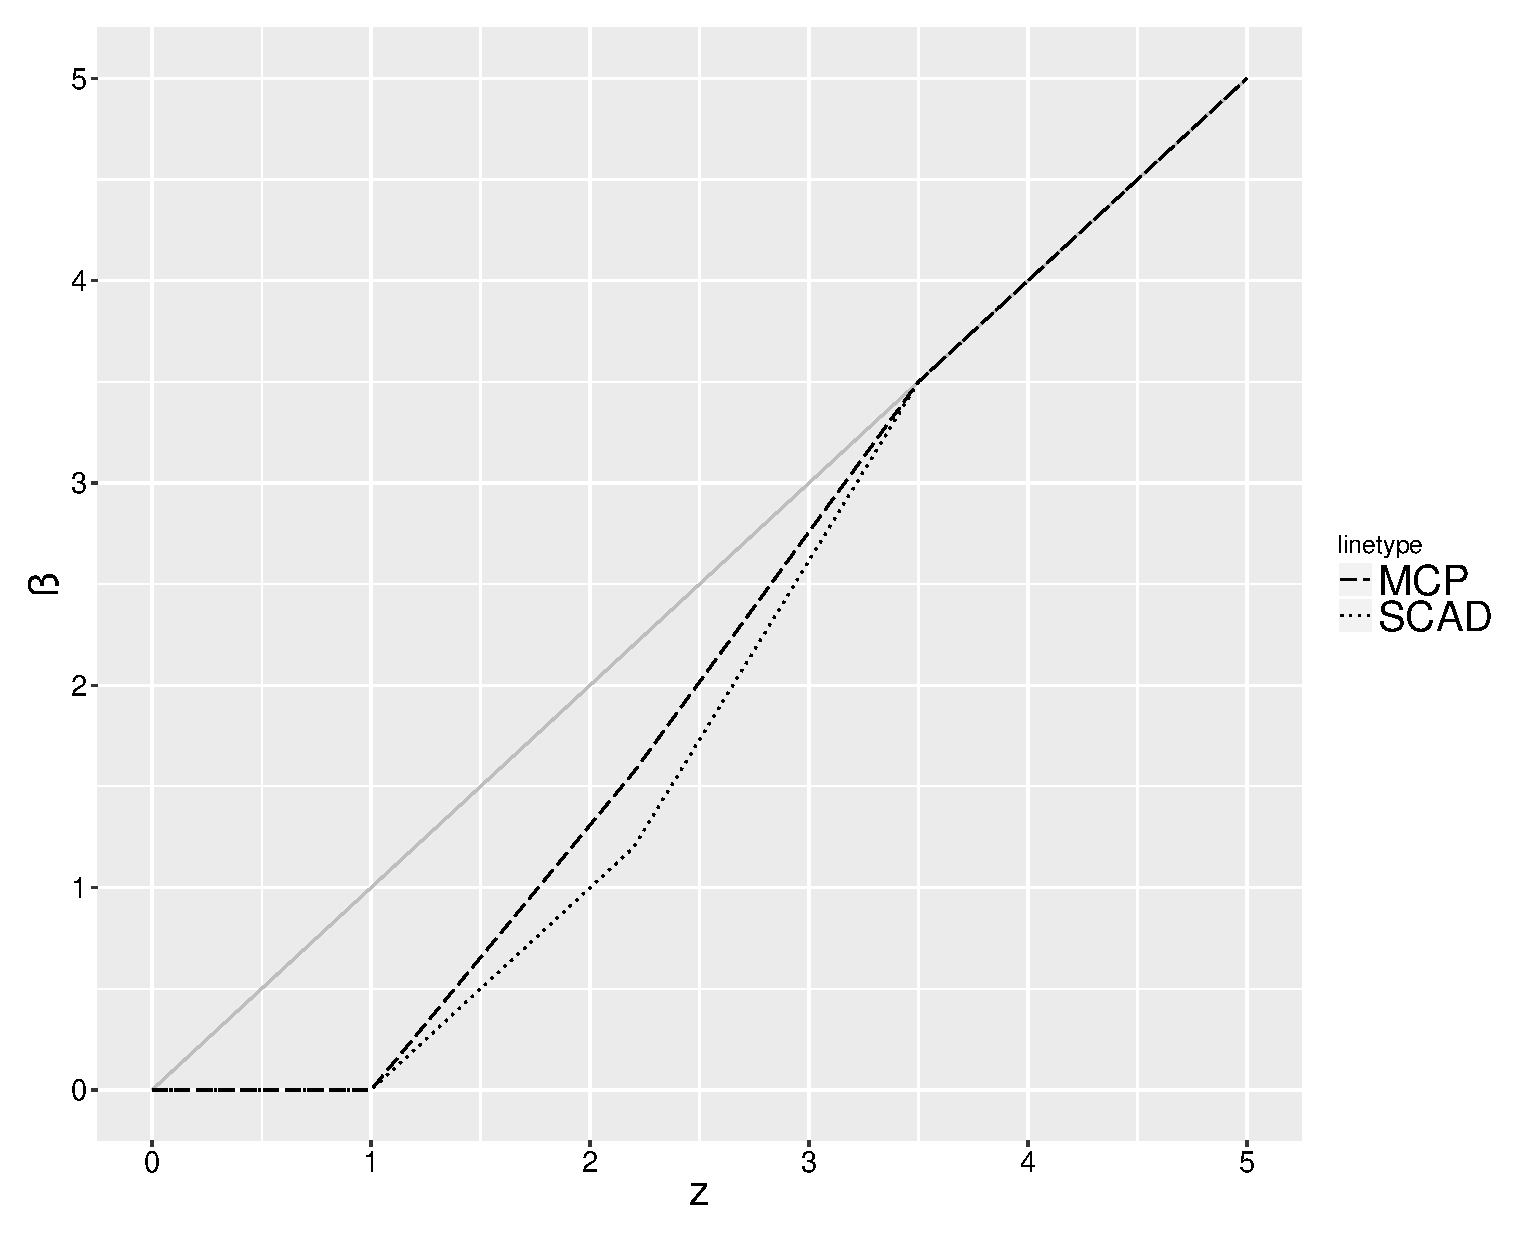
\includegraphics[width = 0.75\textwidth]{R_Plots_penalty_funcrions.eps}
  \captionsetup{font={fivehao}}   %% 这一句放在 caption前面 %%%%%%%% fivehao是前面定义好的10.5pt
  \caption{两种罚函数的图像. }
  \label{fig:Plots of the penalty funcrions} %% label for entire figure
\end{figure}

总结所提出的MMCP方法: 定义惩罚对数似然函数
\begin{equation}
\label{equ:penalized log-likelihood function in MMCP}
  \tilde{l}_{n}(G)=l_{n}(G) + C_{K}\sum_{k=1}^{K}\log\pi_{k} - \sum_{k=1}^{K-1}p_{MCP}(\eta_{k}),
\end{equation}
其中$\log\pi_{k}$对混合比例进行约束, $p_{MCP}(\eta_{k})$对成分的参数之间的距离进行约束. 因此, 通过极大化上式, 可同时实现有限混合模型的定阶及参数估计.

% 如LASSO(\cite{Tibshirani1996Regression})和SCAD(\cite{Fan2001Variable})

\subsection{MMCP方法的数值求解}
下面, 我们对EM算法进行适当修改, 以极大化惩罚对数似然函数(\ref{equ:penalized log-likelihood function in MMCP}).

%$\mathbf{\Psi} = (\theta_1, \theta_2, \ldots, \theta_K, \pi_1, \pi_2, \ldots, \pi_K)$, $\mathbf{\Psi}_0$
记$G = (\pi_1, \pi_2, \ldots, \pi_K, \theta_1, \theta_2, \ldots, \theta_K)$, $G_0$为真实参数值. 给定随机独立样本$\{x_1, x_2, \cdots, x_n\}$, 相应地, 可引入隐变量$\{ \bm{z}_1, \bm{z}_2, \cdots, \bm{z}_n \}$, 指示每个样本所属的成分, 即对于$i \in \{1, 2, \cdots, n\}$, 有$\bm{z}_i = (z_{i1}, z_{i2}, \cdots, z_{iK})^T$, 其中$z_{ik} \in \{ 0, 1 \}$ 且$\sum_{k=1}^{K}z_{ik}=1$. 根据所给样本及其属性(组成的完整数据), 可得惩罚完整对数似然函数
\begin{equation}
\label{equ:penalized complete log-likelihood function}
  \tilde{l}_{n}^{c}(G)=l_{n}^{c}(G) + C_{K}\sum_{k=1}^{K}\log\pi_{k} - \sum_{k=1}^{K-1}p_{MCP}(\eta_{k}),
\end{equation}
其中, $l_{n}^{c}(G)$如式(\ref{equ:complete log-likelihood function})定义.
%\begin{equation}
%\label{equ:complete log-likelihood function}
%  l_{n}^{c}(G)=\sum_{i=1}^{n} \sum_{k=1}^{K} z_{ik} [ \log\pi_{k} + \log\{f(x_{i}; \theta_{k})\} ].
%\end{equation}

E 步中, 在给定观测样本和当前参数估计值$G^{(m)}$ 后, 计算$\tilde{l}_{n}^{c}(G)$关于$z_{ik}$ 的条件期望, 即
\begin{eqnarray}
\label{equ:Q function in revised EM algorithm for MMCP}
  Q(G;G^{(m)}) =&& \sum_{i=1}^{n} \sum_{k=1}^{K} E[z_{ik}|x_i;G^{(m)}] \log\{f(x_{i}; \theta_{k})\}
                   - \sum_{k=1}^{K-1}p_{MCP}(\eta_{k}) \nonumber\\
                && + \sum_{i=1}^{n} \sum_{k=1}^{K} \{ E[z_{ik}|x_i;G^{(m)}] + \frac{C_{K}}{n} \} \log\pi_{k},
\end{eqnarray}
其中,
\begin{equation}
\label{equ:conditional expectation of z_ik in Q function in revised EM algorithm for MMCP}
  E[z_{ik}|x_i;G^{(m)}]
  = \frac{ \pi_k^{(m)} f(x_i; \theta_{k}^{(m)}) }{ \sum_{j=1}^{K} \pi_j^{(m)} f(x_i; \theta_{j}^{(m)}) }.
\end{equation}

M步为求解$G^{(m+1)}=\mathop{\arg\max}_{G} Q(G;G^{(m)})$. 注意到关于混合比例$\pi_k$, 有限制条件$\sum_{j=1}^{K} \pi_j =1$, 应用拉格朗日乘子法, 有
\begin{equation*}
  \frac{\partial [Q(G;G^{(m)})+\lambda(\sum_{j=1}^{K}\pi_j-1)]}{\partial \pi_{k}} =0.
\end{equation*}
可得
\begin{equation*}
  \pi_k^{(m)} = \frac{\sum_{i=1}^{n} E[z_{ik}|x_i;G^{(m)}] + C_{K}}{n + K C_{K}}, k=1, 2, \cdots, K.
\end{equation*}
由于$p_{MCP}(\eta)$不光滑, 无法使用Newton-Raphson方法来关于$\theta_k$极大化$Q(G;G^{(m)})$. 这里, 参考Fan和Li~(2001)的做法, 将$p_{MCP}(\eta)$近似替换为
%FAN J, LI R. Variable selection via nonconvave penalized likelihood and its oracle properties[J]. Journal of the American Statistical Association, 2001, 96(456):1348-1360.
\begin{equation}
\label{equ:replacement of MCP}
  \tilde{p}_{MCP}(\eta;\eta_k^{(m)}) = p_{MCP}(\eta_k^{(m)})+\frac{p'_{MCP}(\eta_k^{(m)})}{2\eta_k^{(m)}}
  (\eta^2-\eta_k^{(m)2}).
\end{equation}
于是, 问题转化为求解如下方程组
\[
\begin{cases}
 \ \sum_{i=1}^{n} E[z_{i1}|x_i;G^{(m)}] \frac{\partial}{\partial \theta_1} \log f(x_i; \theta_{1})
   - \frac{\partial \tilde{p}_{MCP}(\eta_1;\eta_1^{(m)})}{\partial \theta_1}=0, \\
 \ \sum_{i=1}^{n} E[z_{ik}|x_i;G^{(m)}] \frac{\partial}{\partial \theta_k} \log f(x_i; \theta_{k})
   - \frac{\partial \tilde{p}_{MCP}(\eta_{k-1};\eta_{k-1}^{(m)})}{\partial \theta_k}
   - \frac{\partial \tilde{p}_{MCP}(\eta_{k};\eta_{k}^{(m)})}{\partial \theta_k} =0, \\
   \ \hfill k=2, 3, \cdots, K-1, \\
 \ \sum_{i=1}^{n} E[z_{iK}|x_i;G^{(m)}] \frac{\partial}{\partial \theta_K} \log f(x_i; \theta_{K})
   - \frac{\partial \tilde{p}_{MCP}(\eta_{K-1};\eta_{K-1}^{(m)})}{\partial \theta_K}=0.
\end{cases}
\]
将式(\ref{equ:replacement of MCP})带入上述方程组中, 可得
\[
\begin{cases}
 \ \sum_{i=1}^{n} E[z_{i1}|x_i;G^{(m)}] \frac{\partial}{\partial \theta_1} \log f(x_i; \theta_{1})
   + \frac{\partial}{\partial \theta_1} \{ \frac{p'_{MCP}(\eta_1^{(m)})}{2\eta_k^{(m)}}(\theta_{2}-\theta_{1})^2 \} =0, \\
 \ \sum_{i=1}^{n} E[z_{ik}|x_i;G^{(m)}] \frac{\partial}{\partial \theta_k} \log f(x_i; \theta_{k})
   - \frac{\partial}{\partial \theta_k} \{ \frac{p'_{MCP}(\eta_{k-1}^{(m)})}{2\eta_{k-1}^{(m)}}(\theta_{k}-\theta_{k-1})^2 \} \\
   \ \hfill + \frac{\partial}{\partial \theta_k} \{ \frac{p'_{MCP}(\eta_{k}^{(m)})}{2\eta_{k}^{(m)}}(\theta_{k+1}-\theta_{k})^2 \} =0, k=2, 3, \cdots, K-1, \\
 \ \sum_{i=1}^{n} E[z_{iK}|x_i;G^{(m)}] \frac{\partial}{\partial \theta_K} \log f(x_i; \theta_{K})
   - \frac{\partial}{\partial \theta_K} \{ \frac{p'_{MCP}(\eta_{K-1}^{(m)})}{2\eta_{K-1}^{(m)}}(\theta_{K}-\theta_{K-1})^2 \}=0.
\end{cases}
\]
整理, 可得
\[
\begin{cases}
 \ \sum_{i=1}^{n} E[z_{i1}|x_i;G^{(m)}] \frac{\partial}{\partial \theta_1} \log f(x_i; \theta_{1})
   - \frac{p'_{MCP}(\eta_1^{(m)})}{\eta_k^{(m)}}\theta_{2}
   + \frac{p'_{MCP}(\eta_1^{(m)})}{\eta_k^{(m)}}\theta_{1} =0, \\
 \ \sum_{i=1}^{n} E[z_{ik}|x_i;G^{(m)}] \frac{\partial}{\partial \theta_k} \log f(x_i; \theta_{k})
   - \frac{p'_{MCP}(\eta_{k-1}^{(m)})}{\eta_{k-1}^{(m)}}\theta_{k}
   + \frac{p'_{MCP}(\eta_{k-1}^{(m)})}{\eta_{k-1}^{(m)}}\theta_{k-1} \\
   \ \hfill - \frac{p'_{MCP}(\eta_{k}^{(m)})}{\eta_{k}^{(m)}}\theta_{k+1}
   + \frac{p'_{MCP}(\eta_{k}^{(m)})}{\eta_{k}^{(m)}}\theta_{k} =0, k=2, 3, \cdots, K-1, \\
 \ \sum_{i=1}^{n} E[z_{iK}|x_i;G^{(m)}] \frac{\partial}{\partial \theta_K} \log f(x_i; \theta_{K})
   - \frac{p'_{MCP}(\eta_{K-1}^{(m)})}{\eta_{K-1}^{(m)}}\theta_{K}
   + \frac{p'_{MCP}(\eta_{K-1}^{(m)})}{\eta_{K-1}^{(m)}}\theta_{K-1} =0.
\end{cases}
\]
以上方程组包含~$K$~个方程, 求解可得模型的~$K$~个成分参数$\theta_{k}$, $k=1, 2, \cdots, K$.

于是, 任意给定一个参数初始值, $G^{(0)}$. 重复上述E步和M步, 直到参数估计序列收敛, 便可得到参数$G = (\pi_1, \pi_2, \ldots, \pi_K, \theta_1, \theta_2, \ldots, \theta_K)$的估计值, 我们只需将那些$\theta_k$相同的成分对应的混合比例$\pi_k$进行合并, 即可同时完成有限混合模型的定阶与成分参数估计.

下面阐述可调参数的选择问题. 关于$C_{K}$, Chen等~(2001)~指出如果所有成分参数$\theta_k$处于$[-M, M]$或$[M^{-1}, M]$($M$为某个较大的正数)内, 一个合适的取值便是$C_{K}=\log M$. 这里, 我们参考~Xu~和~Chen~(2015)~的做法, 令$M=\max \{x_1, x_2, \cdots, x_n\}$. 关于MMCP惩函数中的$\gamma$和$a$, 前者采用10-折交叉验证选出最优参数, 后者则根据Breheny和Huang~(2011)的建议, 我们令$a=3$.
%CHEN H, CHEN J, KALBFLEISCH J D. A modified likelihood ratio test for homogeneity in finite mixture models[J]. Journal of the Royal Statistical Society: Series B (Statistical Methodology), 2001, 63(1):19-29.
%XU C, CHEN J. A thresholding algorithm for order selection in finite mixture models[J]. Communications in Statistics - Simulation and Computation, 2015, 44(2):433-453.
%BREHENY P, HUANG J. Coordinate descent algorithms for nonconvex penalized regression, with applications to biological feature selection[J]. Annals of Applied Statistics, 2011, 5(1):232-253.

\section{数值实验}
\label{sec:numerical study to MMCP}
为了说明本文所提MMCP方法的性能, 我们将其与MSCAD 在数值实验上进行研究. 下面分别从高斯混合模型和泊松混合模型中产生样本数据并检验两种方法的定阶效果.
%为了说明本文所提MMCP方法的性能, 我们将其与MSCAD 在模拟和实例数据上进行研究. %如果实际数据做好了, 再用这句话来代替!

%\subsection{模拟研究} %如果实际数据做好了, 再加上这个标题!
%我们分别从高斯混合模型和泊松混合模型中产生样本数据.% 模型设定同章节\ref{subsec:simulation study of parameter estimation in finite mixture models using NEW123}.

\textbf{\xiaosihao 例~3.1~}
首先, 我们从如下高斯混合模型的密度函数
\begin{equation*}
  g(x; G)=\sum_{k=1}^{K} \pi_{k} \frac{1}{\sqrt{2\pi}\sigma_{k}} \exp\{-\frac{(x-\mu_{k})^2}{2\sigma_{k}^2}\}.
\end{equation*}
中生成样本数据. 10个模型的参数设定如表\ref{tab:Parameter values for the normal mixture models}所示, 且所有成分的标准差$\sigma_{k}=1$.

可以看出, 在所有混合模型中, 最复杂模型的混合成分个数为$7$, 参考Ishwaran等(2001), 我们令所有模型的成分个数初始值为$15$, 对于那些成分均值之差小于$10^{-3}$的成分, 我们将相应的子群体合并, 同时对混合比例$\pi_k$进行加总~(Xu~和~Chen, 2015).~关于其他参数初始值的设定、迭代终止的准则, 与章节\ref{subsec:simulation study of parameter estimation in finite mixture models using NEW123}~一样.
%ISHWARAN H, JAMES L F, SUN J. Bayesian model selection in finite mixtures by marginal density decompositions[J]. Journal of the American Statistical Association, 2001, 96(456):1316-1332.
%XU C, CHEN J. A thresholding algorithm for order selection in finite mixture models[J]. Communications in Statistics - Simulation and Computation, 2015, 44(2):433-453.

表\ref{tab:Simulation results for normal mixture models with 2 components and known sigma and n = 100}~至表\ref{tab:Simulation results for normal mixture models with 7 components and known sigma and n = 400}~展示了所有高斯混合模型基于500次蒙特卡洛模拟的结果. 可以看出在大部分模型中, MMCP对成分个数$K$的估计准确率都高于MSCAD (除了模型4和模型7, MMCP略低于MSCAD). 特别地, MSCAD方法倾向于将相似子群体合并, 这使得MSCAD对成分数的估计总是偏低, 尤其是当成分参数的距离很近时 (如模型3、模型5、模型8和模型10), 过渡正则化使得MSCAD方法的估计效果很差, 而本文提出的MMCP方法则能较好的对$K$进行估计.

%\begin{table}[h!] %"h", "t", "b" and "p" mean "here", "top", "bottom" and "page". Default is "tbp".
%%\scriptsize  % setting the size of words in the table (from small to large: \tiny \scriptsize \footnotesize \small \normalsize \large \Large \LARGE \huge \Huge )
%\centering
%\caption{两成分高斯混合模型定阶模拟结果old.}
%\label{tab:Simulation results for normal mixture models with 2 components and known sigma and n = 100 old}
%\medskip
%\begin{tabular}{c c c c c c c c}
%\hline  %p{1.2cm}
%  &   & \multicolumn{3}{c}{模型1} & \multicolumn{3}{c}{模型2} \\
%\cmidrule(r){3-5}  \cmidrule(r){6-8}
%$K_0$ & $\hat{K}_0$ & 众数 & MSCAD & MMCP & 众数 & MSCAD & MMCP\\
%\hline
%2 & 1 & 2 & 355 & 83   & 2 & 302 &  38 \\
%   & 2 &    &   77 & 264 &    & 112 & 275 \\
%   & 3 &    &   66 & 130 &    &  85 & 164 \\
%   & 4 &    &     2 &   20 &    &    1 &   21 \\
%   & 5 &    &        &     2 &    &       &     2 \\
%   & 6 &    &        &     1 &    &       &        \\
%\hline
%\end{tabular}
%\end{table}

\begin{table}[h!] %"h", "t", "b" and "p" mean "here", "top", "bottom" and "page". Default is "tbp".
%\scriptsize  % setting the size of words in the table (from small to large: \tiny \scriptsize \footnotesize \small \normalsize \large \Large \LARGE \huge \Huge )
\wuhao
\centering
\captionsetup{font={fivehao}}   %% 这一句放在 caption前面 %%%%%%%% fivehao是前面定义好的10.5pt
\caption{两成分高斯混合模型定阶模拟结果.}
\label{tab:Simulation results for normal mixture models with 2 components and known sigma and n = 100}
\medskip
\begin{tabular}{c c c c c c c c}
%\hline  %p{1.2cm}
\Xhline{1.0pt}
\multirow{2}*{$K_0$} & \multirow{2}*{$\hat{K}$} & \multicolumn{2}{c}{模型1 (众数为2)} & \multicolumn{2}{c}{模型2 (众数为2)} & \multicolumn{2}{c}{模型3 (众数为1)} \\% http://blog.sina.com.cn/s/blog_5e16f1770100u40t.html
\cmidrule(r){3-4} \cmidrule(r){5-6} \cmidrule(r){7-8} % http://www.latexstudio.net/archives/700.html
 &  & MSCAD & MMCP & MSCAD & MMCP & MSCAD & MMCP \\
\hline
  & 1 & 355 & 83 & 302 & 38 & 420 & 299 \\
2 & 2 & 77 & 264 & 112 & 275 & 45 & 99 \\
 & 3 & 66 & 130 & 85 & 164 & 35 & 100 \\
 & 4 & 2 & 20 & 1 & 21 & - & 2 \\
 & 5 & - & 2 & - & 2 & - & - \\
 & 6 & - & 1 & - & - & - & - \\
%\hline
\Xhline{1.0pt}
\end{tabular}
\begin{tablenotes}
  \footnotesize
  \item 注: $K_0$、$\hat{K}$分别表示参数$K$的真实值、估计值, 众数为模型对应的密度函数图像中“峰”的个数. 表中数值代表在500次蒙特卡洛模拟中, 各个方法得到相应$\hat{K}$值的次数, 如355表示在模型1的500次模拟中, MSCAD方法有355次将$K$估计为1. 因此, $K_0$所在行的数值越大, 相应方法的估计效果越好.
\end{tablenotes}
\end{table}

\begin{table}[h!] %"h", "t", "b" and "p" mean "here", "top", "bottom" and "page". Default is "tbp".
%\scriptsize  % setting the size of words in the table (from small to large: \tiny \scriptsize \footnotesize \small \normalsize \large \Large \LARGE \huge \Huge )
\wuhao
\centering
\captionsetup{font={fivehao}}   %% 这一句放在 caption前面 %%%%%%%% fivehao是前面定义好的10.5pt
\caption{四成分高斯混合模型定阶模拟结果.}
\label{tab:Simulation results for normal mixture models with 4 components and known sigma and n = 100}
\medskip
\begin{tabular}{c c c c c c c c}
%\hline  %p{1.2cm}
\Xhline{1.0pt}
\multirow{2}*{$K_0$} & \multirow{2}*{$\hat{K}$} & \multicolumn{2}{c}{模型4 (众数为4)} & \multicolumn{2}{c}{模型5 (众数为1)} & \multicolumn{2}{c}{模型6 (众数为2)} \\
\cmidrule(r){3-4} \cmidrule(r){5-6} \cmidrule(r){7-8}
 &  & MSCAD & MMCP & MSCAD & MMCP & MSCAD & MMCP \\
\hline
 & 1 & 1 & - & 29 & 17 & 14 & 8 \\
 & 2 & 1 & - & 58 & 56 & 80 & 27 \\
 & 3 & 43 & 32 & 388 & 345 & 298 & 261 \\
4 & 4 & 139 & 123 & 21 & 63 & 79 & 130 \\
 & 5 & 226 & 211 & 4 & 19 & 29 & 64 \\
 & 6 & 77 & 95 & - & - & - & 9 \\
 & 7 & 12 & 38 & - & - & - & 1 \\
 & 8 & 1 & 1 & - & - & - & - \\
%\hline
\Xhline{1.0pt}
\end{tabular}
\end{table}

\begin{table}[h!] %"h", "t", "b" and "p" mean "here", "top", "bottom" and "page". Default is "tbp".
%\scriptsize  % setting the size of words in the table (from small to large: \tiny \scriptsize \footnotesize \small \normalsize \large \Large \LARGE \huge \Huge )
\wuhao
\centering
\captionsetup{font={fivehao}}   %% 这一句放在 caption前面 %%%%%%%% fivehao是前面定义好的10.5pt
\caption{七成分高斯混合模型定阶模拟结果.}
\label{tab:Simulation results for normal mixture models with 7 components and known sigma and n = 400}
\medskip
\begin{tabular}{p{0.20cm}<{\centering} p{0.20cm}<{\centering} cccccccc}%{c cccccccc c}
%\hline  %p{1.2cm}
\Xhline{1.0pt}
\multirow{2}*{$K_0$} & \multirow{2}*{$\hat{K}$} & \multicolumn{2}{c}{模型7 (众数为7)} & \multicolumn{2}{c}{模型8 (众数为1)} & \multicolumn{2}{c}{模型9 (众数为3)} & \multicolumn{2}{c}{模型10 (众数为2)} \\
\cmidrule(r){3-4} \cmidrule(r){5-6} \cmidrule(r){7-8} \cmidrule(r){9-10}
 &  & MSCAD & MMCP & MSCAD & MMCP & MSCAD & MMCP & MSCAD & MMCP \\
\hline
 & 2 & - & - & 2 & 2 & - & - & 3 & - \\
 & 3 & - & - & 27 & 18 & 13 & 6 & 27 & 6 \\
 & 4 & 7 & 4 & 73 & 63 & 40 & 26 & 50 & 35 \\
 & 5 & 23 & 18 & 213 & 161 & 167 & 112 & 251 & 158 \\
 & 6 & 44 & 20 & 125 & 116 & 152 & 155 & 77 & 118 \\
7 & 7 & 128 & 98 & 59 & 119 & 92 & 110 & 53 & 110 \\
 & 8 & 88 & 78 & 1 & 12 & 23 & 53 & 17 & 27 \\
 & 9 & 66 & 85 & - & 8 & 12 & 30 & 2 & 24 \\
 & 10 & 28 & 42 & - & 1 & 1 & 7 & 1 & 2 \\
 & 11 & 10 & 36 & - & - & - & 1 & - & 1 \\
 & 12 & 8 & 16 & - & - & - & - & - & - \\
 & 13 & 2 & 7 & - & - & - & - & - & - \\
%\hline
\Xhline{1.0pt}
\end{tabular}
\end{table}

\textbf{\xiaosihao 例~3.2~}
从如下泊松混合模型
\begin{equation*}
  g(x; G)=\sum_{k=1}^{K} \pi_{k} \frac{\theta_k^x}{x!} \exp(-\theta_k).
\end{equation*}
中生成样本数据. 7个模型的参数设定如表\ref{tab:Parameter values for the Poisson mixture models}~所示, 其中每个模型我们均考虑样本量$n=100, 500$两种情形, 并分别进行500次蒙特卡洛模拟.

同样地, 在应用MMCP方法时, 令所有模型的成分个数初始值为$15$, 其他参数初始值的设定及迭代终止的准则, 详见章节\ref{subsec:simulation study of parameter estimation in finite mixture models using NEW123}.

表\ref{tab:Simulation results for Poisson mixture models with 2 components}~至表\ref{tab:Simulation results for Poisson mixture models with 4 components}~展示了所有泊松模型在两种样本量情况下的估计结果. 可以看出, 随着样本量的增大, 两种方法对于模型定阶的准确率都有所提升, 再者, 所有模型中, MMCP对成分数$K$的估计准确率都高于MSCAD.

\begin{table}[h!] %"h", "t", "b" and "p" mean "here", "top", "bottom" and "page". Default is "tbp".
%\scriptsize  % setting the size of words in the table (from small to large: \tiny \scriptsize \footnotesize \small \normalsize \large \Large \LARGE \huge \Huge )
\wuhao
\centering
\captionsetup{font={fivehao}}   %% 这一句放在 caption前面 %%%%%%%% fivehao是前面定义好的10.5pt
\caption{两成分泊松混合模型定阶模拟结果.}
\label{tab:Simulation results for Poisson mixture models with 2 components}
\medskip
\begin{tabular}{c c c c c c c c}
%\hline  %p{1.2cm}
\Xhline{1.0pt}
\multirow{2}*{$K_0$} & \multirow{2}*{$\hat{K}$} & \multicolumn{2}{c}{模型1} & \multicolumn{2}{c}{模型2} & \multicolumn{2}{c}{模型3} \\
\cmidrule(r){3-4} \cmidrule(r){5-6} \cmidrule(r){7-8}
 &  & MSCAD & MMCP & MSCAD & MMCP & MSCAD & MMCP \\
\hline
\multicolumn{2}{c}{$n$=100} &&&&&&\\
\cmidrule(r){1-2}
 & 1 & 446 & 279 & 308 & 59 & 312 & 239 \\
2 & 2 & 54 & 221 & 192 & 441 & 188 & 244 \\
 & 3 & - & - & - & - & - & 17 \\
 \multicolumn{2}{c}{$n$=500} &&&&&&\\
\cmidrule(r){1-2}
 & 1 & 442 & 270 & 252 & 38 & 231 & 191 \\
2 & 2 & 58 & 230 & 248 & 462 & 268 & 308 \\
 & 3 & - & - & - & - & 1 & 1 \\
%\hline
\Xhline{1.0pt}
\end{tabular}
\end{table}

\begin{table}[h!] %"h", "t", "b" and "p" mean "here", "top", "bottom" and "page". Default is "tbp".
%\scriptsize  % setting the size of words in the table (from small to large: \tiny \scriptsize \footnotesize \small \normalsize \large \Large \LARGE \huge \Huge )
\wuhao
\centering
\captionsetup{font={fivehao}}   %% 这一句放在 caption前面 %%%%%%%% fivehao是前面定义好的10.5pt
\caption{三成分泊松混合模型定阶模拟结果.}
\label{tab:Simulation results for Poisson mixture models with 3 components}
\medskip
\begin{tabular}{c c c c c c}
%\hline  %p{1.2cm}
\Xhline{1.0pt}
\multirow{2}*{$K_0$} & \multirow{2}*{$\hat{K}$} & \multicolumn{2}{c}{模型4} & \multicolumn{2}{c}{模型5} \\
\cmidrule(r){3-4} \cmidrule(r){5-6}
 &  & MSCAD & MMCP & MSCAD & MMCP \\
\hline
\multicolumn{2}{c}{$n$=100} &&&&\\
\cmidrule(r){1-2}
 & 1 & 223 & 91 & 166 & 60 \\
 & 2 & 122 & 192 & 220 & 240 \\
3 & 3 & 155 & 217 & 114 & 199 \\
 & 4 & - & - & - & 1 \\
 \multicolumn{2}{c}{$n$=500} &&&&\\
\cmidrule(r){1-2}
 & 1 & 235 & 84 & 148 & 49 \\
 & 2 & 111 & 153 & 295 & 260 \\
3 & 3 & 154 & 262 & 57 & 186 \\
 & 4 & - & 1 & - & 5 \\
%\hline
\Xhline{1.0pt}
\end{tabular}
\end{table}

\begin{table}[h!] %"h", "t", "b" and "p" mean "here", "top", "bottom" and "page". Default is "tbp".
%\scriptsize  % setting the size of words in the table (from small to large: \tiny \scriptsize \footnotesize \small \normalsize \large \Large \LARGE \huge \Huge )
\wuhao
\centering
\captionsetup{font={fivehao}}   %% 这一句放在 caption前面 %%%%%%%% fivehao是前面定义好的10.5pt
\caption{四成分泊松混合模型定阶模拟结果.}
\label{tab:Simulation results for Poisson mixture models with 4 components}
\medskip
\begin{tabular}{c c c c c c}
%\hline  %p{1.2cm}
\Xhline{1.0pt}
\multirow{2}*{$K_0$} & \multirow{2}*{$\hat{K}$} & \multicolumn{2}{c}{模型6} & \multicolumn{2}{c}{模型7} \\
\cmidrule(r){3-4} \cmidrule(r){5-6}
 &  & MSCAD & MMCP & MSCAD & MMCP \\
\hline
\multicolumn{2}{c}{$n$=100} &&&&\\
\cmidrule(r){1-2}
 & 1 & 25 & 6 & 18 & 6 \\
 & 2 & 152 & 124 & 64 & 54 \\
 & 3 & 313 & 304 & 390 & 342 \\
4 & 4 & 10 & 62 & 28 & 80 \\
 & 5 & - & 4 & - & 18 \\
\multicolumn{2}{c}{$n$=500} &&&&\\
\cmidrule(r){1-2}
 & 1 & 38 & 8 & 11 & 4 \\
 & 2 & 134 & 78 & 57 & 38 \\
 & 3 & 300 & 249 & 381 & 282 \\
4 & 4 & 27 & 157 & 45 & 138 \\
 & 5 & 1 & 8 & 6 & 37 \\
 & 6 & - & - & - & 1 \\
%\hline
\Xhline{1.0pt}
\end{tabular}
\end{table}

% 表\ref{tab:Simulation results for normal mixture models 6 with known sigma and n = 100}和表\ref{tab:Simulation results for Poisson mixture models 2}展示了部分模型的结果(由于结果类似, 这里仅展示部分结果. 而所有的模型模拟结果可参见附录). 可以看出, 无论是高斯混合模型, 还是泊松混合模型, MMCP方法相比MSCAD方法在定阶准确率上都有不少提高.
% 附录所有表格的结论: 大部分模型中, MMCP对K的估计准确率都高于MSCAD (除了模型4、7、14, MMCP略低于MSCAD)

%\begin{table}[h!] %"h", "t", "b" and "p" mean "here", "top", "bottom" and "page". Default is "tbp".
%%\scriptsize  % setting the size of words in the table (from small to large: \tiny \scriptsize \footnotesize \small \normalsize \large \Large \LARGE \huge \Huge )
%\centering
%\caption{高斯混合模型定阶模拟结果.}
%\label{tab:Simulation results for normal mixture models 6 with known sigma and n = 100}
%\medskip
%\begin{tabular}{c c c c c c}
%\hline  %p{1.2cm}
%模型 & $K_0$ & 众数 & $\hat{K}_0$ & MSCAD & MMCP \\
%\hline
%6 & 4 & 2 & 1 & 14 & 8  \\
%  &   &   & 2 & 80 & 27 \\
%  &   &   & 3 & 298 & 261 \\
%  &   &   & 4 & 79 & 130 \\
%  &   &   & 5 & 29 & 64 \\
%  &   &   & 6 & 0 & 9 \\
%  &   &   & 7 & 0 & 1 \\
%\hline
%\end{tabular}
%\end{table}

%\begin{table}[h!] %"h", "t", "b" and "p" mean "here", "top", "bottom" and "page". Default is "tbp".
%%\scriptsize  % setting the size of words in the table (from small to large: \tiny \scriptsize \footnotesize \small \normalsize \large \Large \LARGE \huge \Huge )
%\centering
%\caption{泊松混合模型定阶模拟结果.}
%\label{tab:Simulation results for Poisson mixture models 2}
%\medskip
%\begin{tabular}{c c c c c c}
%\hline  %p{1.2cm}
%模型 & $K_0$ & $n$ & $\hat{K}_0$ & MSCAD & MMCP \\
%\hline
%2 & 2 & 100 & 1 & 308 & 59  \\
%  &   &   & 2 & 192 & 441 \\
%  &   & 500 & 2 & 252 & 38 \\
%  &   &   & 2 & 248 & 462 \\
%\hline
%\end{tabular}
%\end{table}

%\subsection{应用实例} %如果实际数据做好了, 再加上这个标题!
%\subsubsection{数据介绍} %如果实际数据做好了, 再考虑加上这个标题!
\section{小结}
本章研究了有限混合模型的定阶问题. 首先, 我们阐述了信息准则法和惩罚最小距离法计算效率低及过拟合的问题; 接着, 基于以上工作, 对惩罚似然方法~(Chen和Khalili, 2008)~进行改进, 提出MMCP方法. 这种方法引入了两个惩罚函数: 一个对混合比例进行约束, 另一个则应用回归模型中变量选择的思想, 对成分参数距离进行约束, 从而解决了两种类型的过拟合. 特别地, MMCP能够同时实现定阶及成分参数的估计. 最后, 数值试验显示, 相比MSCAD方法, MMCP方法对有限混合模型进行定阶的准确率更高.
%CHEN J, KHALILI A. Order selection in finite mixture models with a nonsmooth penalty[J]. Journal of the American Statistical Association, 2008, 103(484):1674-1683.

%https://blog.csdn.net/juechenyi/article/details/77116011
%通常来说, 我们会希望表格的第一根线和最后一根线比表格中的横线更粗一些。
%booktabs 宏包为我们提供了这个功能, 加载 booktabs 宏包之后可以使用 \toprule 和 \bottomrule 命令分别画出表格头和表格底的粗横线, 而用 \midrule 画出表格中的横线。
%%%%%%
%%%%%%\documentclass[UTF8]{ctexart}
%%%%%%\usepackage{booktabs} %需要加载宏包{booktabs}
%%%%%%\begin{document}
%%%%%%
%%%%%%\begin{tabular}{ccc}
%%%%%%\toprule  %添加表格头部粗线
%%%%%%姓名& 学号& 性别\\
%%%%%%\midrule  %添加表格中横线
%%%%%%Steve Jobs& 001& Male\\
%%%%%%Bill Gates& 002& Female\\
%%%%%%\bottomrule %添加表格底部粗线
%%%%%%\end{tabular}
%%%%%%
%%%%%%\end{document}


\chapter[总结与展望]{总结与展望}
\section{总结}
有限混合模型是一种解决复杂分布的工具. 由于几乎所有概率密度都能用有限混合分布逼近, 因此它在理论和应用上均被广泛研究. 作为实际操作中基础又重要的工作, 有限混合混合模型中的参数估计及模型选择比单一模型的复杂得多. 本文便对这两个问题进行研究. 

一方面, 针对有限混合模型的参数估计问题, 本文提出了三种改进的EM算法, 加快了经典EM算法的收敛速度. 通过模拟数据和实际数据分析得出, 新方法对参数估计的准确性和稳定性更高. 另一方面, 针对有限混合模型的定阶问题, 本文提出了MMCP方法, 同时实现混合模型的定阶及其它参数的估计. 相比MSCAD方法, MMCP方法对混合模型的定阶准确率更高.

注意到第二章是在有限混合模型成分个数给定的条件下进行的. 在实际应用中, 有些研究对象可能有较多的理论依据以给出混合模型的成分个数, 或者数据本身可以清晰给出成分个数; 然而有些研究对象则需要事先进行定阶, 我们在例~2.3~中通过将其与AIC和BIC两种信息准则法相结合进行定阶, 但该方法的计算效率依旧有待提升. 第三章提出了MMCP方法, 该方法的数值求解过程较为复杂, 且其渐进性质有待证明, 这些都是值得进一步研究的问题.

\section{未来的工作}
下面展开几个拓展性问题, 即不同成分的混合模型的参数估计、多元混合模型的定阶及算法优化问题.

\subsection{不同成分的混合模型的参数估计}
本文所研究的混合模型可以是高斯混合模型、泊松混合模型、二项混合模型等, 但混合模型中各个子群体的分布是相同. 更为一般化的问题, 是研究不同成分的混合模型. 第二章所提出的三种改进算法的思想依旧是可以应用的. 但是第三章中对子群体分布参数之间的距离进行惩罚的思想, 如何应用到不同成分的混合模型中, 是我们未来将进行的工作.

\subsection{多元混合模型的定阶}
我们所展示的混合模型参数估计及定阶问题都是一元的, 如前文所述, 三种改进的EM算法可以被推广到多元情形, 并且无需额外工作量. 对于MMCP方法, 下面简单阐述改进的方法:

假定随机独立样本$\{\bm{x}_1, \bm{x}_2, \cdots, \bm{x}_n\}$ 均来自多元有限混合模型
\begin{equation*}
  g(\bm{x}; \bm{G})=\sum_{k=1}^{K}\pi_{k}f(\bm{x}; \bm{\theta}_{k}),
\end{equation*}
其中$\bm{G} = (K, \pi_1, \pi_2, \ldots, \pi_K, \bm{\theta}_1, \bm{\theta}_2, \ldots, \bm{\theta}_K)$, $\bm{\theta}_k$为各成分的参数向量. 于是可得对数似然函数
\begin{equation*}
  l_{n}(\bm{G})=\sum_{i=1}^{n}\log\{g(\bm{x}_i; \bm{G})\}.%\{\sum_{k=1}^{K}\pi_{k}f(x_{i}; \theta_{k})\}.
\end{equation*}
本文第三章中, 我们首先对成分参数按大小进行排序, 再将成分参数距离定义为相邻参数的差. 这里, 我们对成分参数重新下定义
\begin{equation*}
  \eta_{k}^{\ast}=\min\{\|\bm{\theta}_{k}-\bm{\theta}_{j}\|: j=k+1, k+2, ..., K\}.
\end{equation*}
可以看出, 本文讨论的情形只是当上式$\bm{\theta}_{k}$取一维的情形. 接着, MMCP方法相应地可改为
\begin{equation*}
  \tilde{l}_{n}(\bm{G})=l_{n}(\bm{G}) + C_{K}\sum_{k=1}^{K}\log\pi_{k} - \sum_{k=1}^{K-1}p_{MCP}(\eta_{k}^{\ast}).
\end{equation*}
我们的想法是: 给定某个较大的$K$值, 最大化上式以完成混合模型的定阶及参数估计, 同时防止两类过拟合情况. 当然此方法的求解也是一个较复杂的难题.

\subsection{算法优化问题}
最值问题一直是被广泛研究的经典问答. 文中第二章提出了三种改进EM算法, 新算法加快了收敛速度, 同时比经典EM算法更加准确及稳定, 但该算法依旧只能收敛到局部最大值, 而不能保证获得全局最大值. 第三章通过修改的EM算法最大惩罚对数似然函数, 该算法一方面需要通过交叉验证进行调参, 另一方在每次迭代的M步都需要求解方程组, 这两者都消耗了大量的计算时间, 同样地, 该算法无法保证收敛到目标函数的全局最大值. 因此, 相关算法的优化问题将是我们未来的工作之一.

\bibliography{bibliography}

%%%%%%%%%%%%%%%%%%%%%%%%%%%%%%%%%%%%%%%%%%%%%%%%%%%%%%%%%%%参考文献
\newpage
\pagestyle{fancy}
\begin{center}
\heiti\sanhao {参考文献}
\end{center}

\addcontentsline{toc}{chapter}{参考文献}

%\begin{itemize}
%  \item [1]] 
%  Xu G, Wang W, He R and Cao J (2018). Modified EM Algorithms for Parameter Estimation in Finite Mixture Models[J]. Communications in Statistics - Theory and Methods, Under Review.       
%  \item [2]]
%  Xu G, Yang S and Wang W (2018). The Ridge Iterative Regression and the Data-Augmentation Lasso[J]. Acta Mathematica Sinica, Under Review.
%  \item [10]]
%  Xu G, Yang S and Wang W (2018). The Ridge Iterative Regression and the Data-Augmentation Lasso[J]. Acta Mathematica Sinica, Under Review.
%\end{itemize}

\begin{enumerate}[{[}1{]}]

\item 	陈希孺, 倪国熙. 数理统计学教程[M]. 合肥: 中国科学技术大学出版社, 2009.
\item 	陈希孺. 高等数理统计学[M]. 合肥: 中国科学技术大学出版社, 2009.
\item 	郑忠国, 童行伟, 赵慧. 高等统计学[M]. 北京: 北京大学出版社, 2012.
\item 	AHMAD K E, JAHEEN Z F, MODHESH A A. Estimation of a discriminant function based on small sample size from a mixture of two gumbel distributions[J]. Communications in Statistics - Simulation and Computation, 2010, 39(4):713-725.
\item 	AKAIKE H. Information theory and an extention of the maximum likelihood principle[C]//Second International Symposium on Information Theory, 1973: 267-281.
\item 	BEHBOODIAN J. On a mixture of normal distributions[J]. Biometrika, 1970, 57(1):215-217.
\item 	BIERNACKI C, CELEUX G, GOVAERT G. Choosing starting values for the EM algorithm for getting the highest likelihood in multivariate Gaussian mixture models[J]. Computational Statistics \& Data Analysis, 2003, 41(3-4):561-575.
\item 	BILMES J A. A gentle tutorial of the EM algorithm and its application to parameter estimation for Gaussian mixture and hidden Markov models[R]. California: TR-97-021, 1998.
\item 	BISHOP C M. Pattern recognition and machine learning (information science and statistics)[M]. New York: Springer-Verlag, Inc, 2006, 430-432.
\item 	BÖHNING D. A review of reliable maximum likelihood algorithms for semiparametric mixture models[J]. Journal of Statistical Planning and Inference, 1995, 47(1-2):5-28.
\item 	BREHENY P, HUANG J. Coordinate descent algorithms for nonconvex penalized regression, with applications to biological feature selection[J]. Annals of Applied Statistics, 2011, 5(1):232-253.
\item 	CHARNIGO R, SUN J. Testing homogeneity in a mixture distribution via the L2 distance between competing models[J]. Journal of the American Statistical Association, 2004, 99(466):488-498.
\item 	CHEN H, CHEN J, KALBFLEISCH J D. A modified likelihood ratio test for homogeneity in finite mixture models[J]. Journal of the Royal Statistical Society: Series B (Statistical Methodology), 2001, 63(1):19-29.
\item 	CHEN H, CHEN J, KALBFLEISCH J D. Testing for a finite mixture model with two components[J]. Journal of the Royal Statistical Society: Series B (Statistical Methodology), 2004, 66(1):95-115.
\item 	CHEN H, CHEN J. Large sample distribution of the likelihood ratio test for normal mixtures[J]. Statistics \& Probability Letters, 2001, 52(2):125-133.
\item 	CHEN H, CHEN J. The likelihood ratio test for homogeneity in finite mixture models[J]. Canadian Journal of Statistics, 2001, 29(2):201-215.
\item 	CHEN J, KALBFLEISCH J D. Penalized minimum‐distance estimates in finite mixture models[J]. Canadian Journal of Statistics, 1996, 24(2):167-175.
\item 	CHEN J, KHALILI A. Order selection in finite mixture models with a nonsmooth penalty[J]. Journal of the American Statistical Association, 2008, 103(484): 1674-1683.
\item 	CHEN J, LI P, FU Y. Inference on the order of a normal mixture[J]. Journal of the American Statistical Association, 2012, 107(499):1096-1105.
\item 	CHEN J, LI P. Testing the order of a normal mixture in mean[J]. Communications in Mathematics and Statistics, 2016, 4(1):21-38.
\item 	CHEN J. On finite mixture models[J]. Statistical Theory and Related Fields, 2017, 1(1):15-27.
\item 	COHEN A C. Estimation in mixtures of two normal distributions[J]. Technometrics, 1967, 9(1):15-28.
\item 	DAY N E. Estimating the components of a mixture of normal distributions[J]. Biometrika, 1969, 56(3):463-474.
\item 	DEMPSTER A P, LAIRD N M, RUBIN D B. Maximum likelihood from incomplete data via the EM algorithm[J]. Journal of the Royal Statistical Society, 1977, 39(1):1-38.
\item 	FAN J, LI R. Variable selection via nonconvave penalized likelihood and its oracle properties[J]. Journal of the American Statistical Association, 2001, 96(456): 1348-1360.
\item 	FIGUEIREDO M A T, JAIN A K. Unsupervised learning of finite mixture models[J]. IEEE Transactions on Pattern Analysis and Machine Intelligence, 2002, 24(3):381-396.
\item 	FU Y, CHEN J, LI P. Modified likelihood ratio test for homogeneity in a mixture of von Mises distributions[J]. Journal of Statistical Planning and Inference, 2008, 138(3):667-681.
\item 	GAREL B. Asymptotic theory of the likelihood ratio test for the identification of a mixture[J]. Journal of Statistical Planning and Inference, 2005, 131(2):271-296.
\item 	GHOSH J K, SEN P K. On the asymptotic performance of the log-likelihood ratio statistic for the mixture model and related results[C]// In Proceedings of the Berkeley conference in Honor of Jerzy Neyman and Jack Kiefer, Volume 2. eds L. LeCam and Richard A. Olshen, 1985:789--806.
\item 	GRIMM K J, MAZZA G L, DAVOUDZADEH P. Model selection in finite mixture models: a k-fold cross-validation approach[J]. Structural Equation Modeling A Multidisciplinary Journal, 2017, 24(2):1-11.
\item 	HASSELBLAD V. Estimation of finite mixtures of distributions from the exponential family[J]. Journal of the American Statistical Association, 1969, 64(328):1459-1471.
\item 	HASSELBLAD V. Estimation of parameters for a mixture of normal distributions[J]. Technometrics, 1966, 8(3):431-444.
\item 	HOLZMANN H, MUNK A, GNEITING T. Identifiability of finite mixtures of elliptical distributions[J]. Scandinavian Journal of Statistics, 2006, 33(4):753–763.
\item 	HOLZMANN H, MUNK A, STRATMANN B. Identifiability of finite mixtures - with applications to circular distributions[J]. Sankhyā: The Indian Journal of Statistics (2003-2007), 2004, 66(3):440-449.
\item 	ISHWARAN H, JAMES L F, SUN J. Bayesian model selection in finite mixtures by marginal density decompositions[J]. Journal of the American Statistical Association, 2001, 96(456):1316-1332.
\item 	JAMES L F, PRIEBE C E, MARCHETTE D J. Consistent estimation of mixture complexity[J]. Annals of Statistics, 2001:1281-1296.
\item 	KIM D, SEO B. Assessment of the number of components in Gaussian mixture models in the presence of multiple local maximizers[J]. Journal of Multivariate Analysis, 2014, 125(125):100-120.
\item 	LEHMANN, E L. Theory of point estimation[M]. New York: JohnWiley, 1998.
\item 	LEROUX B G. Consistent estimation of a mixing distribution[J]. The Annals of Statistics, 1992:1350-1360.
\item 	LI P, CHEN J. Testing the order of a finite mixture[J]. Journal of the American Statistical Association, 2010, 105(491):1084-1092.
\item 	LIU C, RUBIN D B. The ECME algorithm: a simple extension of EM and ECM with faster monotone convergence[J]. Biometrika, 1994, 81(4):633-648.
\item 	LOUIS T A. Finding the observed information matrix when using the EM algorithm[J]. Journal of the Royal Statistical Society. Series B (Methodological), 1982: 226-233.
\item 	MCLACHLAN G J. The EM algorithm and extensions(second edition)[M]. New York: Wiley \& Sons, Inc, 2008, 61-65.
\item 	MELNYKOV V, MELNYKOV I. Initializing the EM algorithm in Gaussian mixture models with an unknown number of components[J]. Computational Statistics \& Data Analysis, 2012, 56(6):1381-1395.
\item 	MENG X L, RUBIN D B. Maximum likelihood estimation via the ECM algorithm: A general framework[J]. Biometrika, 1993, 80(2):267-278.
\item 	NEYMAN J, SCOTT E L. On the Use of C($\alpha$) optimal tests of composite hypothesis[J]. Bulletin of the International Statistical Institute, 1966, 41(1):477--497.
\item 	PEARSON K. Contribution to the mathematical theory of evolution[J]. Philosophical Transactions of the Royal Society of London A, 1894, 186:71-110.
\item 	PENG W. Model selection for Gaussian mixture model based on desirability level criterion[J]. Optik - International Journal for Light and Electron Optics, 2016, 130:797-805.
\item 	RICHARDSON S, GREEN P J. On Bayesian analysis of mixtures with an unknown number of components[J]. Journal of the Royal Statistical Society, 1997, 59(4):731-792.
\item 	ROEDER K. Density estimation with confidence sets exemplified by superclusters and voids in the galaxies[J]. Journal of the American Statistical Association, 1990, 85(411):617-624.
\item 	SARAIVA E F, LOUZADA F, MILAN L. Mixture models with an unknown number of components via a new posterior split–merge MCMC algorithm[J]. Applied Mathematics \& Computation, 2014, 244(2):959-975.
\item 	SCHWARZ G. Estimating the dimension of a model[J]. The Annals of Statistics, 1978, 6(2):461-464.
\item 	ŠTEPÁNOVÁ K, VAVREČKA M. Estimating number of components in Gaussian mixture model using combination of greedy and merging algorithm[J]. Pattern Analysis \& Applications, 2016:1-12.
\item 	TEICHER H. Identifiability of finite mixtures[J]. Annals of Mathematical Statistics, 1963, 34(4):1265-1269.
\item 	TEICHER H. On the mixture of distributions[J]. Annals of Mathematical Statistics, 1960, 31(1):55-73.
\item 	TIBSHIRANI, R. Regression shrinkage and selection via the lasso[J]. Journal of the Royal Statistical Society: Series B (Methodological), 1996:267-288.
\item 	UEDA N, NAKANO R. Deterministic annealing EM algorithm[M]. Elsevier Science Ltd. 1998:271–282.
\item 	WEI G C G, Tanner M A. A Monte Carlo implementation of the EM algorithm and the poor man's data augmentation algorithms[J]. Journal of the American Statistical Association, 1990, 85(411):699-704.
\item 	WOO M J, SRIRAM T. Robust estimation of mixture complexity for count data[J]. Computational Statistics and Data Analysis, 2007, 51(9):4379-4392.
\item 	WU C F J. On the convergence properties of the EM algorithm[J]. The Annals of Statistics, 1983: 95-103.
\item 	XU C, CHEN J. A thresholding algorithm for order selection in finite mixture models[J]. Communications in Statistics - Simulation and Computation, 2015, 44(2):433-453.
\item 	YIN J, ZHANG Y, GAO L. Accelerating expectation-maximization algorithms with frequent updates[C]// IEEE International Conference on CLUSTER Computing. IEEE, 2012:275-283.
\item 	YU J, CHAOMURILIGE C, YANG M S. On convergence and parameter selection of the EM and DA-EM algorithms for Gaussian mixtures[J]. Pattern Recognition, 2018, 77: 188-203.
\item 	ZHANG C H. Nearly unbiased variable selection under minimax concave penalty[J]. Annals of Statistics, 2010, 38(2):894-942.

\end{enumerate}

%%%%%%%%%%%%%%%%%%%%%%%%%%%%%%%%%%%%%%%%%%%%%%%%%%%%%%%%%%%参考文献

%%%%%%%%%%%%%%%%%%%%%%%%%%%%%%%%%%%%%%%%%%%%%%%%%%%%%%%%%%%硕士研究生期间的科研成果
\newpage
\pagestyle{fancy}
\begin{center}
\heiti\sanhao {硕士研究生期间的科研成果}
\end{center}

\addcontentsline{toc}{chapter}{硕士研究生期间的科研成果}

论文:

\textbf{XU G}, WANG W, He R, Cao J. Modified EM algorithms for parameter estimation in finite mixture models[J]. Communications in Statistics - Theory and Methods, 2018, Under Review.

\textbf{XU G}, YANG S, WANG W. The ridge iterative regression and the data-augmentation lasso[J]. Acta Mathematica Sinica, 2018, Under Review.

\

课题:

混合模型及改进EM算法的理论与应用. 浙江省自然科学基金 Y19A010012. 排名: 3/5.

\

竞赛:

第十四届中国研究生数学建模竞赛. 二等奖. 排名: 2/3.

第十三届全国研究生数学建模竞赛. 三等奖. 排名: 1/3.

%%%%%%%%%%%%%%%%%%%%%%%%%%%%%%%%%%%%%%%%%%%%%%%%%%%%%%%%%%%硕士研究生期间的科研成果



%%%%%%%%%%%%%%%%%%%%%%%%%%%%%%%%%%%%%%%%%%%%%%%%%%%%%%%%%%%%%%%
\newpage
\pagestyle{fancy}
\begin{center}
\heiti\sanhao {致\quad 谢}
\end{center}

\addcontentsline{toc}{chapter}{致谢}

在论文完整之际, 我想感谢硕士研究生阶段所有帮助和支持我的老师、同学和亲友们.

首先, 我要感谢我的导师王伟刚老师. 无论在科研还是工作生活中, 王老师都给了我很大的指导和鼓励. 读研以来, 我前进的每一步背后都倾注了王老师大量的心血. 王老师学识渊博、功底深厚, 对于科学问题总有独到的见解, 本文的不少创新点正是在与老师的讨论当中诞生的. 尽管王老师平日里要负责学院里的工作和繁重的教学任务, 但他对于科研的认真态度从不懈怠, 对于学生的学习和生活也时常放在心上. 非常幸运能在硕士研究生阶段跟着王老师学习, 师恩难忘, 在此向王老师表示最诚挚的感谢!

其次, 我要感谢讨论班的明瑞星老师、董雪梅老师. 明老师的科研态度严谨认真, 能够全面深刻地看待问题, 在课上、讨论班上总能提出创新、专业的观点, 明老师对于本论文的选题和创新点也提供了很大的帮助; 董老师为人和蔼, 经常在讨论班对学生的疑问作出透彻的解释, 给出很多相应的解决方案. 未来的学习和工作中, 我将以老师们为榜样不断前进.

此外, 我要感谢在讨论班一起学习的肖敏学姐、李亚旭学长以及各位同学. 肖学姐和李学长对我论文写作过程中的指导, 让我获益匪浅. 也要感谢班里的同学, 在平时一起学习、打球、游泳, 使我的生活充满了乐趣.

最后, 感谢我家人、朋友、亲戚, 在我读研期间给我的生活提供了各方面的关怀, 使我保持良好的状态投入到学业中.

再次感谢所有帮助我的人们!


%%%%%%%%%%%%%%%%%%%%%%%%%%%%%%%%%%%%%%%%%%%%%%%
%\newpage
%\thispagestyle{empty}
%\begin{center}\heiti\sanhao\textbf{独\ 创\ 性\ 声\ 明}\end{center}
%\begin{spacing}{2.0}
%本人声明所呈交的学位论文是本人在导师指导下进行的研究工作及取得的研究成果.尽我所知,除了文中特别加以标注和致谢的地方外,论文中不包含其他人已经发表或撰写过的研究成果,也不包含本人为获得浙江工商大学或其它教育机构的学位或证书而使用过的材料.与我一同工作的同志对本研究所做的任何贡献均已在论文中作了明确的说明并表示谢意.\\
%
%~~~~~~~~~~~~~~~~~~签名:\underline{\hspace{3cm} }\ \ 日期: \hspace{0.8cm} 年 \hspace{0.2cm} 月 \hspace{0.4cm} 日\\
%%~~~~~~~~~~~~~~~~~~签名:\underline{\hspace{0.8cm} 许耿鑫 \hspace{0.8cm}}\ \ 日期: 2018 年 1 月 14 日\\
%\\
%
%\begin{center}\heiti\sanhao\textbf{ 关于论文使用授权的说明}\end{center}
%~~~~~~本学位论文作者完全了解浙江工商大学有关保留、使用学位论文的规定:浙江工商大学有权保留并向国家有关部门或机构送交论文的复印件和磁盘,允许论文被查阅和借阅,可以将学位论文的全部或部分内容编入有关数据库进行检索,可以采用影印、缩印或扫描等复制手段保存、汇编学位论文,并且本人电子文档的内容和纸质论文的内容相一致.
%
%保密的学位论文在解密后也遵守此规定.\\
%
%~~~~~~~~~~~~~~~~~~签名:\underline{\hspace{3cm} }\ \ 导师签名:\underline{\hspace{3cm}}
%%~~~~~~~~~~~~~~~~~~签名:\underline{\hspace{0.8cm} 许耿鑫 \hspace{0.8cm}}\ \ 导师签名:\underline{\hspace{0.8cm} 王伟刚 \hspace{0.8cm}}
%
%~~~~~~~~~~~~~~~~~~~~~~~~~~~~~~~~~~~~~~~~~~~~~~~~~~~ 日期: \hspace{0.8cm} 年 \hspace{0.2cm} 月 \hspace{0.4cm} 日
%%~~~~~~~~~~~~~~~~~~~~~~~~~~~~~~~~~~~~~~~~~~~~~~~~~~~ 日期: 2018 年 1 月 14 日
%\end{spacing}
%%%%%%%%%%%%%%%%%%%%%%%%%%%%%%%%%%%%%%%%%%%%%%%%%%%%%%%%%%%%%%%%%%%%%%%%%%%%%


\end{document}





